\documentclass[12pt,twoside]{article}
\newcommand{\reporttitle}{ElasticFusion on the Google Tango Tablet}
\newcommand{\reportauthor}{Jiahao Lin}
\newcommand{\reporttype}{Final Year Project Report}
\newcommand{\cid}{00837321}
\newcommand{\email}{jiahao.lin13@imperial.ac.uk}
\newcommand{\supervisor}{Dr Stefan Leutenegger}
\newcommand{\secondmarker}{Professor Andrew Davison}
\newcommand{\tabincell}[2]{\begin{tabular}{@{}#1@{}}#2\end{tabular}}

\usepackage{listings}

\lstset{
  basicstyle=\ttfamily,
  columns=fullflexible,
  frame=single,
  breaklines=true,
  postbreak=\mbox{\textcolor{red}{$\hookrightarrow$}\space},
}



% include files that load packages and define macros
%%%%%%%%%%%%%%%%%%%%%%%%%%%%%%%%%%%%%%%%%
% University Assignment Title Page 
% LaTeX Template
% Version 1.0 (27/12/12)
%
% This template has been downloaded from:
% http://www.LaTeXTemplates.com
%
% Original author:
% WikiBooks (http://en.wikibooks.org/wiki/LaTeX/Title_Creation)
%
% License:
% CC BY-NC-SA 3.0 (http://creativecommons.org/licenses/by-nc-sa/3.0/)
% 
% Instructions for using this template:
% This title page is capable of being compiled as is. This is not useful for 
% including it in another document. To do this, you have two options: 
%
% 1) Copy/paste everything between \begin{document} and \end{document} 
% starting at \begin{titlepage} and paste this into another LaTeX file where you 
% want your title page.
% OR
% 2) Remove everything outside the \begin{titlepage} and \end{titlepage} and 
% move this file to the same directory as the LaTeX file you wish to add it to. 
% Then add \input{./title_page_1.tex} to your LaTeX file where you want your
% title page.
%
%----------------------------------------------------------------------------------------
%	PACKAGES AND OTHER DOCUMENT CONFIGURATIONS
%----------------------------------------------------------------------------------------
\usepackage{ifxetex}
\usepackage{textpos}
\usepackage{natbib}
\usepackage{kpfonts}
\usepackage[a4paper,hmargin=2.8cm,vmargin=2.0cm,includeheadfoot]{geometry}
\usepackage{ifxetex}
\usepackage{stackengine}
\usepackage{tabularx,longtable,multirow,subfigure,caption}%hangcaption
\usepackage{fncylab} %formatting of labels
\usepackage{fancyhdr}
\usepackage{color}
\usepackage[tight,ugly]{units}
\usepackage{url}
\usepackage{float}
\usepackage[english]{babel}
\usepackage{amsmath}
\usepackage{graphicx}
\usepackage[colorinlistoftodos]{todonotes}
\usepackage{dsfont}
\usepackage{epstopdf} % automatically replace .eps with .pdf in graphics
\usepackage{natbib}
\usepackage{backref}
\usepackage{array}
\usepackage{latexsym}
\usepackage{etoolbox}

\usepackage{enumerate} % for numbering with [a)] format 



\ifxetex
\usepackage{fontspec}
\setmainfont[Scale=.8]{OpenDyslexic-Regular}
\else
\usepackage[pdftex,pagebackref,hypertexnames=false,colorlinks]{hyperref} % provide links in pdf
\hypersetup{pdftitle={},
  pdfsubject={}, 
  pdfauthor={\reportauthor},
  pdfkeywords={}, 
  pdfstartview=FitH,
  pdfpagemode={UseOutlines},% None, FullScreen, UseOutlines
  bookmarksnumbered=true, bookmarksopen=true, colorlinks,
    citecolor=black,%
    filecolor=black,%
    linkcolor=black,%
    urlcolor=black}
\usepackage[all]{hypcap}
\fi

\usepackage{tcolorbox}

% various theorems
\usepackage{ntheorem}
\theoremstyle{break}
\newtheorem{lemma}{Lemma}
\newtheorem{theorem}{Theorem}
\newtheorem{remark}{Remark}
\newtheorem{definition}{Definition}
\newtheorem{proof}{Proof}

% example-environment
\newenvironment{example}[1][]
{ 
\vspace{4mm}
\noindent\makebox[\linewidth]{\rule{\hsize}{1.5pt}}
\textbf{Example #1}\\
}
{ 
\noindent\newline\makebox[\linewidth]{\rule{\hsize}{1.0pt}}
}



%\renewcommand{\rmdefault}{pplx} % Palatino
% \renewcommand{\rmdefault}{put} % Utopia

\ifxetex
\else
\renewcommand*{\rmdefault}{bch} % Charter
\renewcommand*{\ttdefault}{cmtt} % Computer Modern Typewriter
%\renewcommand*{\rmdefault}{phv} % Helvetica
%\renewcommand*{\rmdefault}{iwona} % Avant Garde
\fi

\setlength{\parindent}{0em}  % indentation of paragraph

\setlength{\headheight}{14.5pt}
\pagestyle{fancy}
\fancyfoot[ER,OL]{\thepage}%Page no. in the left on
                                %odd pages and on right on even pages
\fancyfoot[OC,EC]{\sffamily }
\renewcommand{\headrulewidth}{0.1pt}
\renewcommand{\footrulewidth}{0.1pt}
\captionsetup{margin=10pt,font=small,labelfont=bf}


%--- chapter heading

\def\@makechapterhead#1{%
  \vspace*{10\p@}%
  {\parindent \z@ \raggedright %\sffamily
        %{\Large \MakeUppercase{\@chapapp} \space \thechapter}
        %\\
        %\hrulefill
        %\par\nobreak
        %\vskip 10\p@
    \interlinepenalty\@M
    \Huge \bfseries 
    \thechapter \space\space #1\par\nobreak
    \vskip 30\p@
  }}

%---chapter heading for \chapter*  
\def\@makeschapterhead#1{%
  \vspace*{10\p@}%
  {\parindent \z@ \raggedright
    \sffamily
    \interlinepenalty\@M
    \Huge \bfseries  
    #1\par\nobreak
    \vskip 30\p@
  }}
  



% %%%%%%%%%%%%% boxit
\def\Beginboxit
   {\par
    \vbox\bgroup
	   \hrule
	   \hbox\bgroup
		  \vrule \kern1.2pt %
		  \vbox\bgroup\kern1.2pt
   }

\def\Endboxit{%
			      \kern1.2pt
		       \egroup
		  \kern1.2pt\vrule
		\egroup
	   \hrule
	 \egroup
   }	

\newenvironment{boxit}{\Beginboxit}{\Endboxit}
\newenvironment{boxit*}{\Beginboxit\hbox to\hsize{}}{\Endboxit}



\allowdisplaybreaks

\makeatletter
\newcounter{elimination@steps}
\newcolumntype{R}[1]{>{\raggedleft\arraybackslash$}p{#1}<{$}}
\def\elimination@num@rights{}
\def\elimination@num@variables{}
\def\elimination@col@width{}
\newenvironment{elimination}[4][0]
{
    \setcounter{elimination@steps}{0}
    \def\elimination@num@rights{#1}
    \def\elimination@num@variables{#2}
    \def\elimination@col@width{#3}
    \renewcommand{\arraystretch}{#4}
    \start@align\@ne\st@rredtrue\m@ne
}
{
    \endalign
    \ignorespacesafterend
}
\newcommand{\eliminationstep}[2]
{
    \ifnum\value{elimination@steps}>0\leadsto\quad\fi
    \left[
        \ifnum\elimination@num@rights>0
            \begin{array}
            {@{}*{\elimination@num@variables}{R{\elimination@col@width}}
            |@{}*{\elimination@num@rights}{R{\elimination@col@width}}}
        \else
            \begin{array}
            {@{}*{\elimination@num@variables}{R{\elimination@col@width}}}
        \fi
            #1
        \end{array}
    \right]
    & 
    \begin{array}{l}
        #2
    \end{array}
    &%                                    moved second & here
    \addtocounter{elimination@steps}{1}
}
\makeatother

%% Fast macro for column vectors
\makeatletter  
\def\colvec#1{\expandafter\colvec@i#1,,,,,,,,,\@nil}
\def\colvec@i#1,#2,#3,#4,#5,#6,#7,#8,#9\@nil{% 
  \ifx$#2$ \begin{bmatrix}#1\end{bmatrix} \else
    \ifx$#3$ \begin{bmatrix}#1\\#2\end{bmatrix} \else
      \ifx$#4$ \begin{bmatrix}#1\\#2\\#3\end{bmatrix}\else
        \ifx$#5$ \begin{bmatrix}#1\\#2\\#3\\#4\end{bmatrix}\else
          \ifx$#6$ \begin{bmatrix}#1\\#2\\#3\\#4\\#5\end{bmatrix}\else
            \ifx$#7$ \begin{bmatrix}#1\\#2\\#3\\#4\\#5\\#6\end{bmatrix}\else
              \ifx$#8$ \begin{bmatrix}#1\\#2\\#3\\#4\\#5\\#6\\#7\end{bmatrix}\else
                 \PackageError{Column Vector}{The vector you tried to write is too big, use bmatrix instead}{Try using the bmatrix environment}
              \fi
            \fi
          \fi
        \fi
      \fi
    \fi
  \fi 
}  
\makeatother

\robustify{\colvec}

%%% Local Variables: 
%%% mode: latex
%%% TeX-master: "notes"
%%% End: 
 % various packages needed for maths etc.
% quick way of adding a figure
\newcommand{\fig}[3]{
 \begin{center}
 \scalebox{#3}{\includegraphics[#2]{#1}}
 \end{center}
}

%\newcommand*{\point}[1]{\vec{\mkern0mu#1}}
\newcommand{\ci}[0]{\perp\!\!\!\!\!\perp} % conditional independence
\newcommand{\point}[1]{{#1}} % points 
\renewcommand{\vec}[1]{{\boldsymbol{{#1}}}} % vector
\newcommand{\mat}[1]{{\boldsymbol{{#1}}}} % matrix
\newcommand{\R}[0]{\mathds{R}} % real numbers
\newcommand{\Z}[0]{\mathds{Z}} % integers
\newcommand{\N}[0]{\mathds{N}} % natural numbers
\newcommand{\nat}[0]{\mathds{N}} % natural numbers
\newcommand{\Q}[0]{\mathds{Q}} % rational numbers
\ifxetex
\newcommand{\C}[0]{\mathds{C}} % complex numbers
\else
\newcommand{\C}[0]{\mathds{C}} % complex numbers
\fi
\newcommand{\tr}[0]{\text{tr}} % trace
\renewcommand{\d}[0]{\mathrm{d}} % total derivative
\newcommand{\inv}{^{-1}} % inverse
\newcommand{\id}{\mathrm{id}} % identity mapping
\renewcommand{\dim}{\mathrm{dim}} % dimension
\newcommand{\rank}[0]{\mathrm{rk}} % rank
\newcommand{\determ}[1]{\mathrm{det}(#1)} % determinant
\newcommand{\scp}[2]{\langle #1 , #2 \rangle}
\newcommand{\kernel}[0]{\mathrm{ker}} % kernel/nullspace
\newcommand{\img}[0]{\mathrm{Im}} % image
\newcommand{\idx}[1]{{(#1)}}
\DeclareMathOperator*{\diag}{diag}
\newcommand{\E}{\mathds{E}} % expectation
\newcommand{\var}{\mathds{V}} % variance
\newcommand{\gauss}[2]{\mathcal{N}\big(#1,\,#2\big)} % gaussian distribution N(.,.)
\newcommand{\gaussx}[3]{\mathcal{N}\big(#1\,|\,#2,\,#3\big)} % gaussian distribution N(.|.,.)
\newcommand{\gaussBig}[2]{\mathcal{N}\left(#1,\,#2\right)} % see above, but with brackets that adjust to the height of the arguments
\newcommand{\gaussxBig}[3]{\mathcal{N}\left(#1\,|\,#2,\,#3\right)} % see above, but with brackets that adjust to the height of the arguments
\DeclareMathOperator{\cov}{Cov} % covariance (matrix) 
\ifxetex
\renewcommand{\T}[0]{^\top} % transpose
\else
\newcommand{\T}[0]{^\top}
\fi
% matrix determinant
\newcommand{\matdet}[1]{
\left|
\begin{matrix}
#1
\end{matrix}
\right|
}



%%% various color definitions
\definecolor{darkgreen}{rgb}{0,0.6,0}

\newcommand{\blue}[1]{{\color{blue}#1}}
\newcommand{\red}[1]{{\color{red}#1}}
\newcommand{\green}[1]{{\color{darkgreen}#1}}
\newcommand{\orange}[1]{{\color{orange}#1}}
\newcommand{\magenta}[1]{{\color{magenta}#1}}
\newcommand{\cyan}[1]{{\color{cyan}#1}}


% redefine emph
\renewcommand{\emph}[1]{\blue{\bf{#1}}}

% place a colored box around a character
\gdef\colchar#1#2{%
  \tikz[baseline]{%
  \node[anchor=base,inner sep=2pt,outer sep=0pt,fill = #2!20] {#1};
    }%
}%
 % short-hand notation and macros

%%%%%%%%%%%%%%%%%%%%%%%%%%%%

\begin{document}

% front page
% Last modification: 2016-09-29 (Marc Deisenroth)
\begin{titlepage}

\newcommand{\HRule}{\rule{\linewidth}{0.5mm}} % Defines a new command for the horizontal lines, change thickness here


%----------------------------------------------------------------------------------------
%	LOGO SECTION
%----------------------------------------------------------------------------------------


\includegraphics[width = 4cm]{./figures/imperial}\\[0.5cm]

\begin{center} % Center remainder of the page

%----------------------------------------------------------------------------------------
%	HEADING SECTIONS
%----------------------------------------------------------------------------------------
\textsc{\LARGE \reporttype}\\[1.5cm]
\textsc{\Large Imperial College London}\\[0.5cm]
\textsc{\large Department of Computing}\\[0.5cm]
%----------------------------------------------------------------------------------------
%	TITLE SECTION
%----------------------------------------------------------------------------------------

\HRule \\[0.4cm]
{ \huge \bfseries \reporttitle}\\ % Title of your document
\HRule \\[1.5cm]
\end{center}
%----------------------------------------------------------------------------------------
%	AUTHOR SECTION
%----------------------------------------------------------------------------------------

%\begin{minipage}{0.4\hsize}
\begin{flushleft} \large
\textit{Author:}\\
\reportauthor~(CID: \cid) % Your name
\\Supervisor: \supervisor\\
\end{flushleft}
\vspace{2cm}
\makeatletter
Date: \@date

\vfill % Fill the rest of the page with whitespace



\makeatother


\end{titlepage}


%%%%%%%%%%%%%%%%%%%%%%%%%%%% Main document

\section{Abstract}
Abstract\\
The abstract is a very brief summary of the report's contents. It should be about half a page long. Somebody unfamiliar with your project should have a good idea of what it's about having read the abstract alone and will know whether it will be of interest to them. Note that the abstract is a summary of the entire project including its conclusions. A common mistake is to provide only introductory elements in the abstract without saying what has been achieved.\\

=============\\                                                                                                                                                                                                                                                                                                                                                                                                                                                                                                                                                                                                                                                                                                                                                                                                                                                                                                                                                                                                                         Google Tango\cite{tango} is an augmented reality computing platform by Google that give mobile devices the ability to sense 3D space information. Equipped with this platform Google's Tango tablet is an Android device that carry sensors including 4MP(Mega Pixel) color camera, Inertial Measurement Unit (IMU), and Infra-Red depth camera. it also carrys NVIDIA Tegra K1 processor which provides more powerful computational power than other mobile devices. Given this cheap commodity mobile hardware and software, this project aims to build a fully self-contained 3D dense surface reconstruction solution using  state-of-the-art RGB-D(color and depth) SLAM (Simultaneous Localization And Mapping) algorithms.\\
\\
In the recently published dense RGB-D SLAM algorithms, ElasticFusion\cite{whelan2016elasticfusion} published by Dyson Robotics Lab\footnote{\url{http://www.imperial.ac.uk/dyson-robotics-lab/}} at Imperial College London is one that achieve state-of-the-art performance by applying local and global loop closures using a deformation graph, so that drifts raised by accumulated errors can be recovered and global consistency of the map is maintained. The fact Elastic Fusion scored high marks on benchmarks for trajectory estimation and surface estimation makes it perfect to be applied on Google Tango Tablet. Also, the current code exist for ElasticFusion running on desktop computer made heavily use of CUDA(Compute Unified Device Architecture) for GPU general data processing, which is supported by the NVIDIA Tegra K1 processer on Google Tango tablet.\\
\\
This project have attempted to port the code for ElasticFusion onto Google Tango Tablet and integrated with 3D points data from Tango platform, although the result of running ElasticFusion on the tablet has shown to be not effective enough for self-contained real time application due to processing power and sensor problem on the tablet and time and effort limitation in this project, this attempt has still proved that it is possible and more convenient to record the 3D space data on a hand held portable device first, and then let the data to be processed on a more power desktop computer for high quality 3D surface reconstruction.\\
\\
Also, since the Tango platform on the tablet provides pose estimation feature, this pose is simply feed into the ElasticFusion program run on the tablet, so that the ElasticFusion part doesn't need to waste time and processing power to execute the camera tracking part. However, the pose provided by Tango may not be accurate enough and during the reconstruction process ElasticFusion will alter the pose if global or local loop closure happens, in this project a simply way to correct pose input to ElasticFusion by Tango is developed to  over come this problem.

%%%%%%%%%%%%%%%%%%%%%%%%%%%%

\newpage

\section{Acknowledgements}
Firstly I would like to express my deepest appreciation to all those who provided me the possibility to complete this report. A special gratitude I give to my project supervisor, Dr. Stefan Leutenegger, for his patient overseeing and guidance throughout this project, also his time and effort invested to give useful advices.\\
\\
Secondly I would also like to thank my friends for accepting nothing less than excellence from me. Last but not the least, I would like to thank my parents for supporting me spiritually throughout the progress of this project and my life in general.

\newpage

%%%%%%%%%%%%%%%%%%%%%%%%%%%%

\tableofcontents

%%%%%%%%%%%%%%%%%%%%%%%%%%%%

\newpage

\section{Introduction}

This is one of the most important components of the report. It should begin with a clear statement of what the project is about so that the nature and scope of the project can be understood by a lay reader. It should summarise everything you set out to achieve, provide a clear summary of the project's background, relevance and main contributions. It should explain the motivation for the project (i.e., why the problem is important) and identify the issues to be addressed (i.e., why the problem is difficult). The introduction should set the scene for the project and should provide the reader with a summary of the key things to look out for in the remainder of the report. When detailing the contributions it is helpful to provide pointers to the section(s) of the report that provide the relevant technical details. The introduction itself should be largely non-technical. It is sometimes useful to state the main objectives of the project as part of the introduction. However, avoid the temptation to list low-level objectives one after another in the introduction and then later, in the evaluation section (see below), say something like "All the objectives of the project have been met blah blah...". A project that meets all its objectives is, by definition, weak and unambitious. Concentrate instead on the big issues, e.g. the main questions (scientific or otherwise) that the project sets out to answer.\\

=============\\


==========\\

The main objective of this project is to develop a fully self-contained mobile dense 3D surface reconstruction solution running on Google Tango Tablet using the ElasticFusion algorithm. Ideally the 3D surface reconstructed should be rendered on screen in real time from the tablet's viewpoint when user is holding the tablet to scan the room, and after the scanning stopped the 3D map created should be able saved on device to allow for later use or shown on other devices. The motivation of behind this project is the lacking of high quality 3D surface reconstruction application on mobile device. Applications for 3D reconstruction currently exist on Tango Platform mostly use volumetric representation, and can only produce coarse model of surrounding space, a screen shot of using 3D mesh created using Google Tango's demo mesh builder application is shown in Fig \ref{fig:ScreenshotTango5}. Also the existing applications fail to produce surface map without misalignments during the scanning process, which is often caused by loopy motion of the scanning device in the process. When doing 3D reconstruction, simple fusion of 3D point clouds would produce drifts caused by errors accumulating over time, therefore by applying ElasticFusion algorithm to the solution, even extremely loopy trajectories of the tablet and long duration of scanning process would not result in decrease of accuracy of the map. On the contrary, revisit areas that has previously been mapped will only help to maintain the global consistency of the map. The part of algorithm that made this possible in ElasticFusion is the local and   global loop closure checking after camera tracking process, which will be discussed in detail later.\\
\begin{figure}[h]
    \centering
    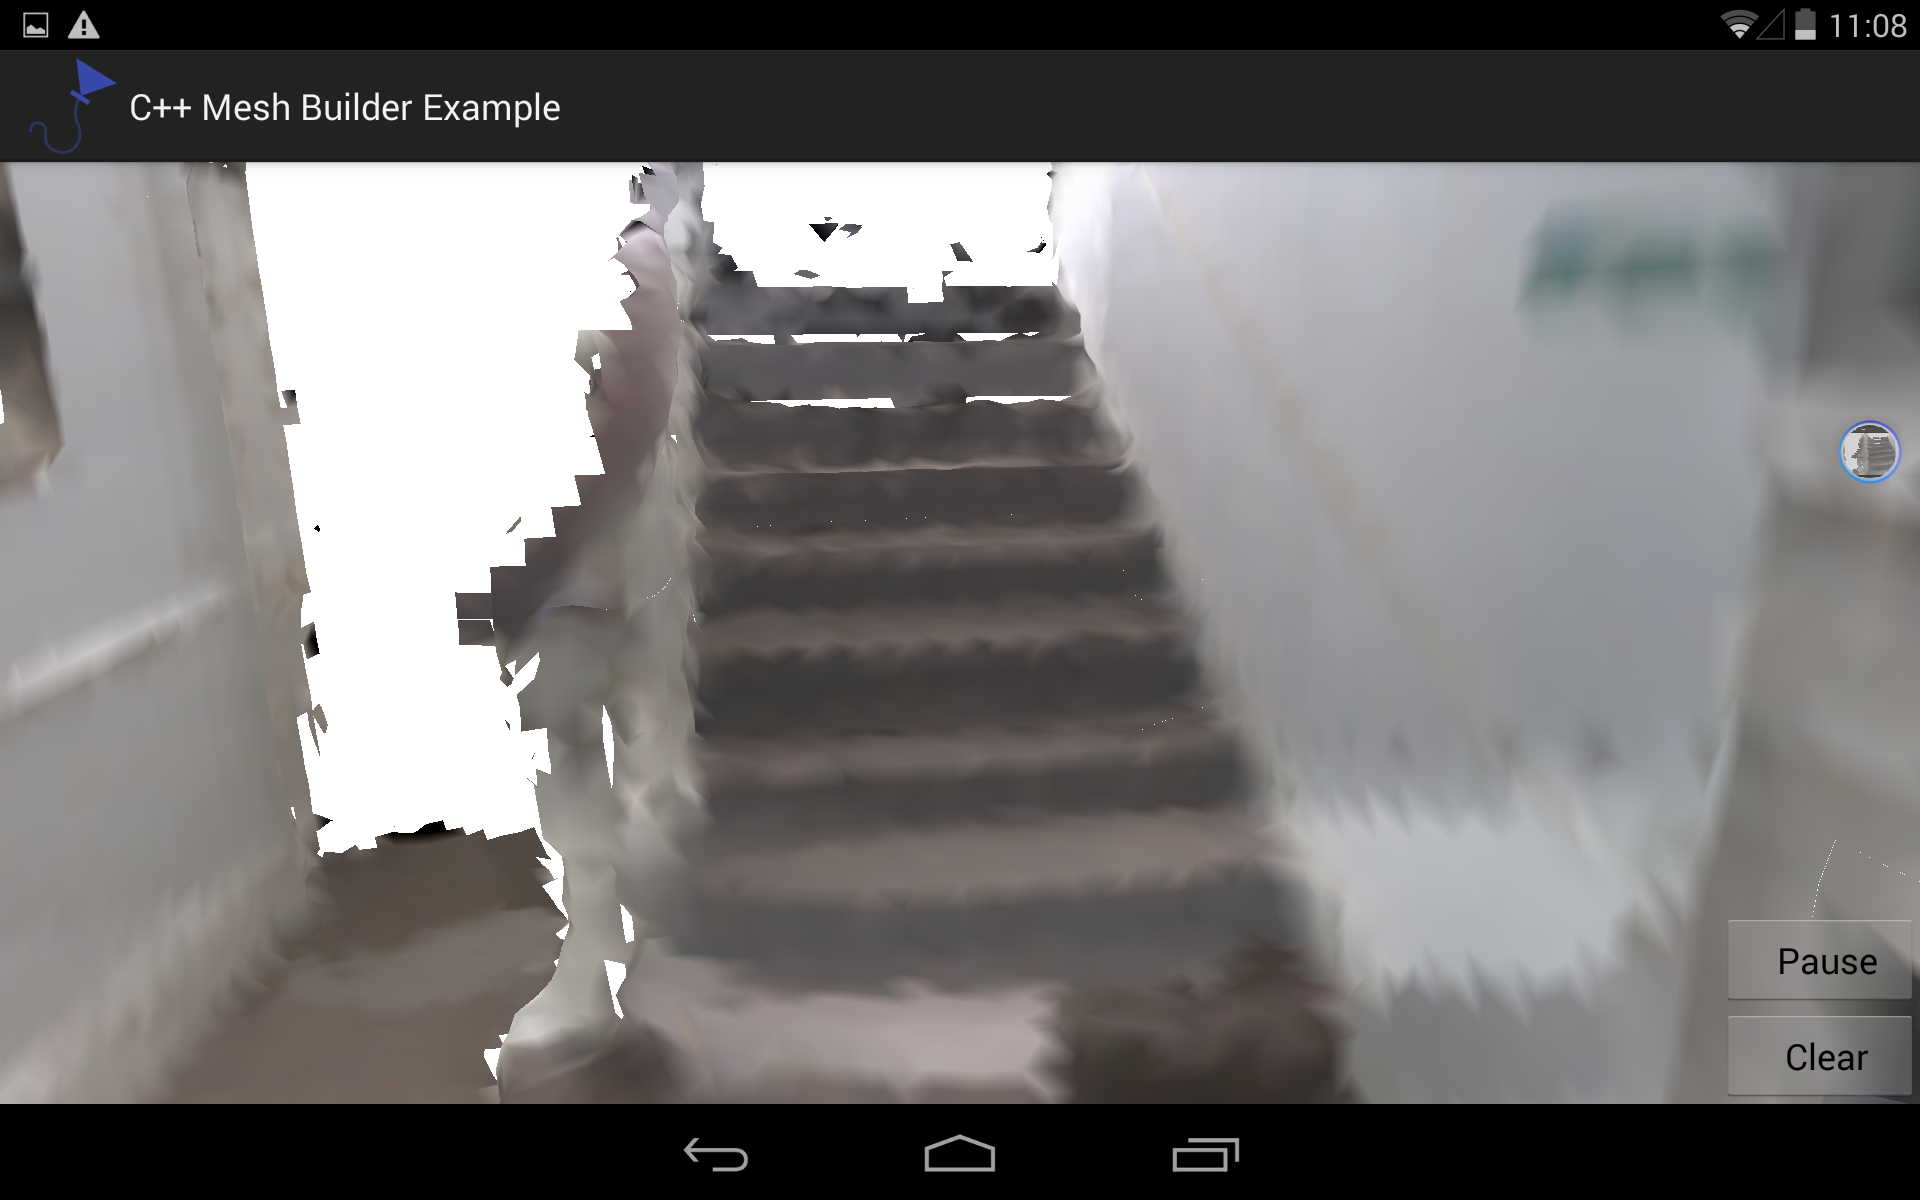
\includegraphics[width=0.7\textwidth]{figures/ScreenshotTango5}
    \caption{ScreenshotTango5}
    \label{fig:ScreenshotTango5}
\end{figure}
Previously, ElasticFusion can only be run on a desktop computer with powerful graphic card, using a raw dataset that is given, or connect the computer to a RGB-D camera such as Microsoft Kinect or ASUS Xtion Pro Live or Intel RealSense 3D Camera. That makes it non convenient for a user to scan the space he or she is currently in for 3D reconstruction, therefore the Google Tango tablet with both RGB and depth camera would be the perfect mobile device to implement a portable version of ElasticFusion on. The Google Tango tablet carries Android 4.2.2 OS, has 4GB of RAM, a quadcore Nvidia Tegra K1 graphics card supporting CUDA, six-axis gyroscope and accelerometer, a wide-angle 120 field of view tracking camera which refreshes at 60Hz, a projective depth sensor which refreshes at 3Hz, and a 4 megapixel color sensor which refreshes at 30Hz. The processing power on this tablet succeeds most mobile devices on the market right now, which makes running ElasticFusion on the device alone become possible. Since ElasticFusion requires both high end processor and graphic card on a desktop computer, from the read me of ElasticFusion on Github: "A very fast nVidia GPU (3.5 TFLOPS+), and a fast CPU (something like an i7)." is recommended for a desktop computer, therefore one of important problem in this project is that Tango tablet's processing power is still not strong enough to run ElasticFusion for real time application. However, the attempt make in this project have still shown the possibility of running a state of the art SLAM  algorithm on mobile device.\\
\\
In the original design for this project, if the development of this solution is successful, an augmented reality application could be created as demo to illustrate the interaction of virtual object with scanned 3D surface map. But after various experiments in this project, a conclusion that ElasticFusion could not be run on Tango tablet as a real time application drawn, due to processing power and depth sensor accuracy problem, although due to time and effort limitations, the ElasticFusion on Tango application produces in this project still produce incorrect reconstruction model and the program has not been optimized. Despite all the above, the contribution of this project still includes the attempt made to implement this solution, and the possibility of using Tango tablet as a pure scanning device for recording data, and let the data to be processed on other computers for doing 3D surface reconstruction.\\
\\
In the solution, an Android application is developed using Android Native Development Kit (NDK)\footnote{\url{https://developer.android.com/ndk/index.html}}, which allows the use of Tango C API\footnote{\url{https://developers.google.com/tango/apis/c/}} to acquire depth camera data and 3D pose data, also makes it possible to reuse the existing code for ElasticFusion that is written in C++. Therefore most of the application is written in C++, with a few Java code for the Android application. The application uses the code for Advanced Estimation in Robotics (433H) course practical exercise by Dr Stefan Leutenegger in Department of Computing at Imperial College London as the basic frame work, firstly the code is combined with the logger for ElasticFusion\footnote{\url{https://github.com/mp3guy/Logger1}} to write the RGB, depth and pose data in format required by ElasticFusion acquired from Tango into two files on the Tango tablet, which allows ElasticFusion to be run on desktop using these two files as raw dataset. Then the core function part of code for ElasticFusion is ported and adapted to Android with its dependencies changed or removed, so that ElasticFusion can be run on Android while its source remains in C++. One thing worth notice in here is that this project uses an internal version of ElasticFusion source code at Dyson Robotics Lab in Imperial College London, instead of the open source version on Github\footnote{\url{https://github.com/mp3guy/ElasticFusion}}. The final produced application is able to log the data from sensors on Tango into files, or run ElasticFusion from sensor data in real time, or run ElasticFusion from raw dataset files on the device with or without pose data. This provides various way to do experiments or measure  efficiency during the project. However, due to time and effort limitations, no interface for showing the progress of ElasticFusion running is built, this is different from original planning but the reasons will be explain in detail later. Right now on the screen of the application, interface only shows the image that color camera is taking and a few buttons, screen shot and description will be provided in later section.\\
\\
Finally, simple change is made on both desktop version and Android version of ElasticFusion to allow for pose feed into the program to be corrected overtime when global or local loop closure happens. This help maintain consistency between the pose feed into ElasticFusion and the internal pose stored in the program. Since the original ElasticFusion can only estimate pose from RGB-D data, or use an input pose as ground truth pose, or use the input pose as a bootstrap pose for optimization, the adaptation made in this project enables the pose feed into ElasticFusion to be consistent with the true pose while also not waste time to do the camera tracking process when the processing power is not so strong like on the Tango tablet.


\newpage


\section{Background}
The background section of the report should set the project into context by relating it to existing published work which you read at the start of the project when your approach and methods were being considered. There are usually many ways of solving a given problem, and you shouldn't just pick one at random. Describe and evaluate as many alternative approaches as possible. The published work may be in the form of research papers, articles, text books, technical manuals, or even existing software or hardware of which you have had hands-on experience. Your must acknowledge the sources of your inspiration. You are expected to have seen and thought about other people's ideas; your contribution will be putting them into practice in some other context. However, avoid plagiarism: if you take another person's work as your own and do not cite your sources of information/inspiration you are being dishonest; in other words you are cheating. When referring to other pieces of work, cite the sources where they are referred to or used, rather than just listing them at the end. Make sure you read and digest the Department's plagiarism document .\\
In writing the Background chapter you must demonstrate your capability of analysis, synthesis and critical judgement. Analysis is shown by explaining how the proposed solution operates in your own words as well as its benefits and consequences. Synthesis is shown through the organisation of your Related Work section and through identifying and generalising common aspects across different solutions. Critical judgement is shown by discussing the limitations of the solutions proposed both in terms of their disadvantages and limits of applicability.\\
Typically you can look for Background work using different search engines including:\\
* Google Scholar
* IEEExplore
* ACM Digital Library
* Citeseer
* Science Direct
Note 1: Often the terms Background, Related Work or State of the Art are used interchangeably.\\
Note 2: Keyword search is wonderful, but you need the right Keywords.\\
Note 2: IEEExplore, ACM Digital Library and Science Direct require you to be on the College network to download the PDF of papers. If at home, use VPN.\\

=============\\

This section includes two parts, the first part includes some paper related to SLAM and SLAM algorithm including ElasticFusion, the second part includes some SLAM applications developed to be run on mobile devices.\\

\subsection{SLAM papers}


\subsubsection{Past, Present, and Future of Simultaneous Localization And Mapping: Towards the Robust Perception Age}
This survey paper: past present and future of SLAM \cite{cadena2016past} gave a detail description about the current development state of modern SLAM, including standard formulation and models, different methods used in SLAM. Below we give a brief summary of basic knowledge about SLAM from this paper.\\
\\
Simultaneous Localization and Mapping (SLAM) means constructing the model of environment (map) that the robot is in, and estimating the robot state within the environment at the same time. Usually the robot is equipped with some kind of sensor: RGB camera, depth sensor, IMU, or GPS, So that the robot is able to perceive the environment in some way from these sensor. In standard models, the robot state includes its position and orientation, velocity, sensor biases and calibration parameter. Using the robot status and  data read from sensors, the environment(map) constructed could be representation in different forms. With the existence of the map, errors raised in estimating robot state could be eliminated and also doing "loop closure" when robot revisits a place in the map allows drift to be corrected and hence improve accuracy of the estimated status of robot.\\
\begin{figure}[h]
    \centering
    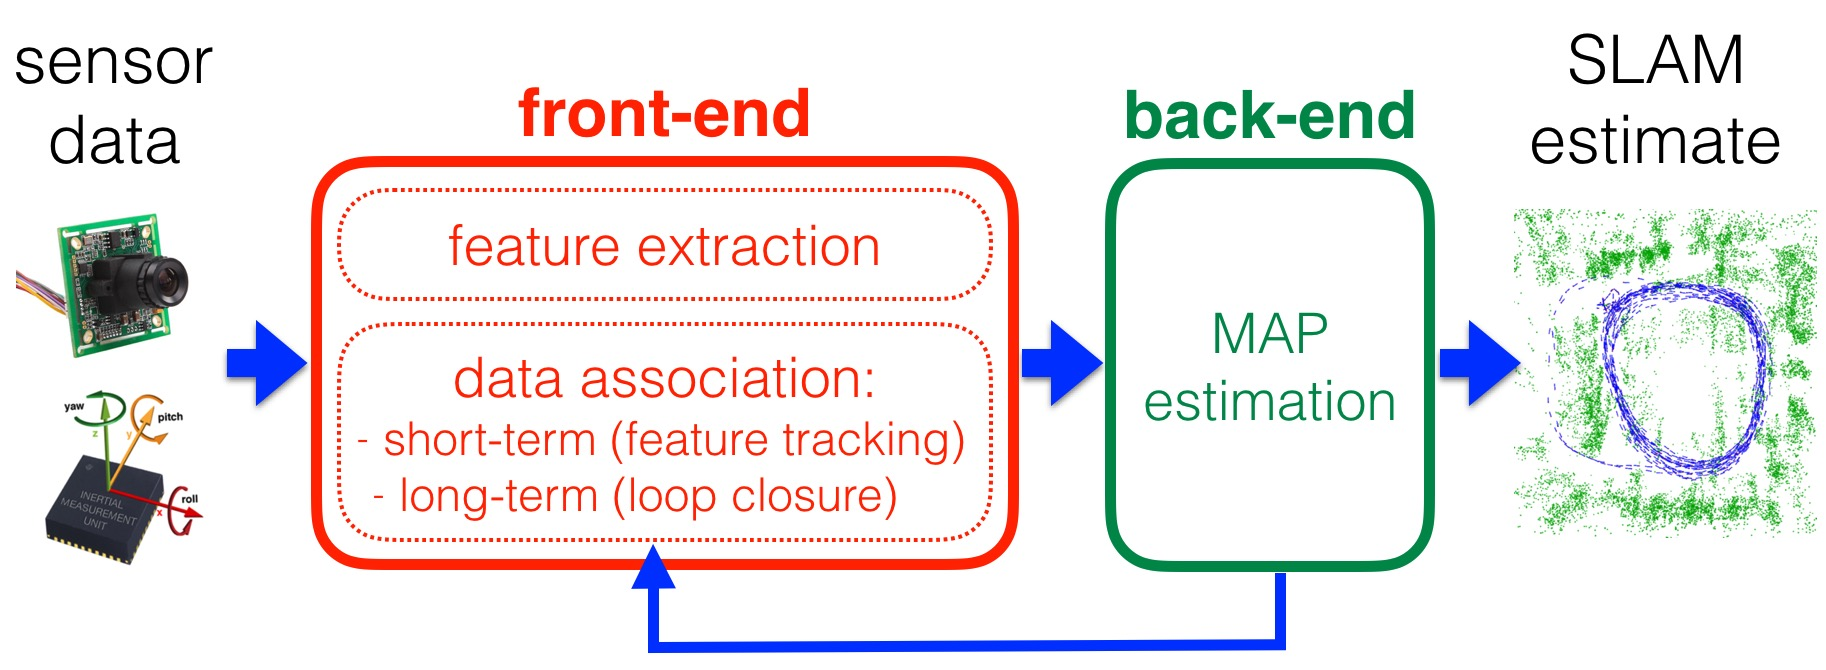
\includegraphics[width=0.7\textwidth]{figures/slamStructure}
    \caption{Front-end and back-end in a typical SLAM system\cite{cadena2016past}}
    \label{fig:slamStructure}
\end{figure}
\\The structure of SLAM system is mainly divided into two parts: front-end and back-end
The front-end extract features from sensor data and associate them to the model used to make predictions, then the back-end does estimation of robot state and the map using this model produced by front-end. As you can see in the figure \ref{fig:slamStructure}, this process forms a continuous process of tracking and update.\\
\\
Classical formulations of SlAM is to take probabilistic approaches such as models based on Maximum Likelihood Estimation, Maximum-a-posteriori (MAP) estimation, EKF(Extended Kalman Filters), and particle filters.\\
Many of the popular SLAM algorithm models it as a maximum-a-posteriori estimation problem  by taking probability approach. And usually using a factor graph to show relationships and constraints between variables. In these models, often an observation or measurement model is used to represent the probability of observe measurements given the state of robot, given some random measurement noise that usually model to be under a zero-mean Gaussian distribution. By using Bayes theorem, the MAP estimate, in which the posterior is the probability of robot state given a measurement, can be calculated given some prior belief of the robot state. In the case that there is no prior information known about robot state, the MAP estimate would simply become a maximum-likelihood-estimate. When we are given a set of independent robot states and measurements, these variable would become factors(nodes) in the factor graph, and their probabilistic relationships would become the constraints(edges) in the factor graph.\\
\\
Factor graph allows us to visualize our problem in a simple way and provides an insight into how the variables are related together by their constraints. \ref{fig:factorgraph} from the paper have shown an example of it for a simple SLAM problem.
\\
\begin{figure}[h]
    \centering
    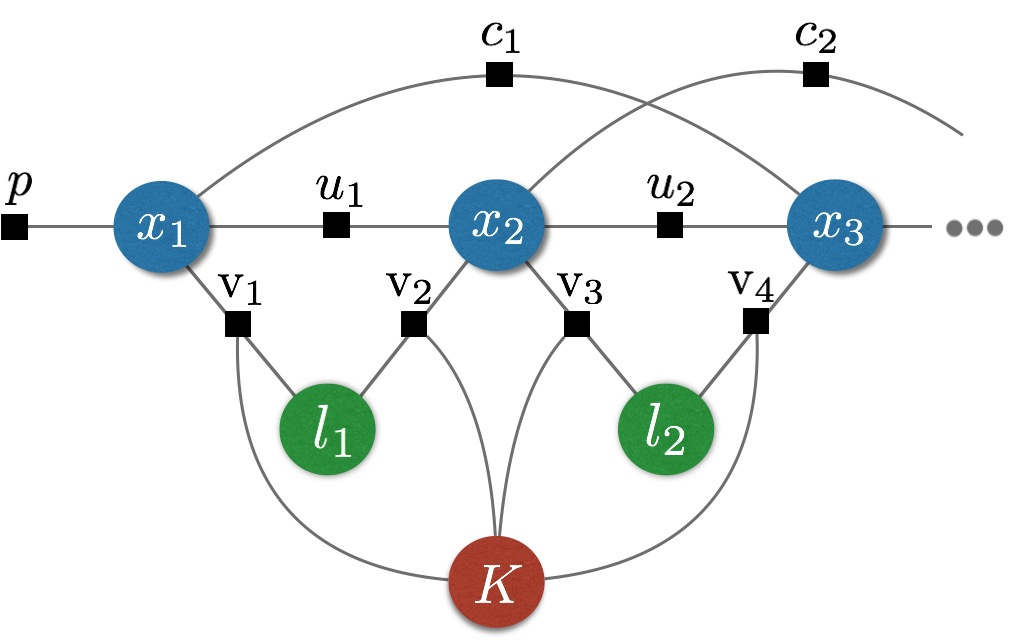
\includegraphics[width=0.7\textwidth]{figures/factorgraph}
    \caption{SLAM as a factor graph\cite{cadena2016past}}
    \label{fig:factorgraph}
\end{figure}
\\
As explained in \cite{cadena2016past}: \lq\lq Blue circles denote robot poses at
consecutive time steps ($x1$, $x2$ ...), green circles denote landmark positions
($l1$, $l2$ ...), red circle denotes the variable associated with the intrinsic
calibration parameters ($K$). Factors are shows are black dots: the label \lq\lq $u$\rq\rq marks factors corresponding to odometry constraints, \lq\lq $v$ \rq\rq marks factors corresponding to camera observations, \lq\lq $c$\rq\rq denotes loop closures, and \lq\lq $p$\rq\rq denotes prior factors."\\
\\
When calculating the MAP estimate of robot state, we can transform the problem into minimizing the negative log of posterior, assuming the noise is zero-mean Gaussian distributed, this becomes a non-linear least squares problem, since we will be minimising the measurement error's $l2$ norm. This method is similar to the BA (Bundle Adjustment) method in computer vision area, which minimise the reprojection error. However factor graph can not only contain visual and geometry factor, but also a variety of data from different sensors. Also the MAP estimate is calculated every time a measurement is arrived, instead of performing calculation  after all the data is given.\\
\\
Different from factor graph optimization, a similar approach is called pose graph optimization, which estimate trajectory of robot using measurements between relative poses as constraints, and optimized these poses to achieve better accuracy trajectory.\\
\\
Other than optimization-based estimation, some filtering approach using EKF model have also achieve great results, such as MSCKF(Multi-State Constraint Kalman Filter of Mourikis and Roumeliotis)\cite{mourikis2007multi}, EKF is used for performing filtering on the linearised point of estimate, and have shown to be accurate in visual-inertial navigation.\\
\\
In terms of the representation of the map, one way is to have a group of features or landmarks in 3D, these features are usually extracted from sensor images to be allow easy distinguishable from environment, such as edges and corners. The method used to extracting features from images are well-established within computer vision area, using descriptors like ROB, SIFT, and SURF. The discriminative and repetitive properties of landmarks allow the correspondence of each landmark and sensor measurement(image), and then via triangulating, the robot is able to compute the relative pose between measurements and geometric information about landmarks, therefore achieve localization and mapping.\\
\\
Other than feature based approach, sometimes raw dense representation of the environment is used. different than extracting landmarks, this approach stores a dense 3D map using high resolution points, the 3D geometry of environment is described by these vast amount of points, so called point clouds. With stereo or depth cameras, lase r depth sensors, 3D information of the points can be easily obtained, therefore this method is popular in RGB-D SLAM. Sometimes, these points doesn't only stores simple 3D information, in Elasticfusion\citep{whelan2016elasticfusion}, each 3D point is represented by a surfel, which is a disk with certain radius centred by the 3D point and stored information such as normal vector of that point on the surface and color. These suefel disk combine together can encode the geometry of environment better than simple points.\\
At more a higher level than raw, unstructured points, dense related element that partitioned by space is also used to represent surface and boundaries, such as surface mesh models(connected polygons formed by points) and implicit surface representations like octree and occupancy grid. KinectFusion\citep{newcombe2011kinectfusion} storing surfaces using volumetric representation by uniformly subdivide a 3D physical space into a 3D grid of fixed size voxels, voxels defining surface has a zeros value of the truncated signed-distance function (TSDF) function that stores distance information relative to the surface. We can see that represent the environment in these types of dense data requires huge amount of storage, however they give very low level geometry information which is suitable for 3D reconstruction and rendering.\\
\\
Comparing feature-based and dense SLAM methods, for the purpose of this project, dense SLAM algorithm Elasticfusion\citep{whelan2016elasticfusion} is used as 3D reconstruction is the main objective instead of state estimation, since Elasticfusion maintains a dense 3D surfel map that make use of all the information about the environment obtained from sensors it is more robust in localization and mapping that feature-based approaches.\\





\subsubsection{Kinectfusion}
KinectFusion\cite{newcombe2011kinectfusion} is a dense RGB-D SLAM method that enables high quality 3D reconstruction and interaction in real time. This method make use of low cost mobile RGB-D camera, scanning the environment in real time and acquire 3D point information about the space. During the reconstruction process, holes caused by absence of depth measurement in original 3D point cloud is filled in, and the model is refined by repetitive scanning over time.\\
\\
Firstly the 3D points reading are then stored in a 3D vertex map and their normal vectors are calculated by reprojection of neighbouring vertexes. After that the camera pose is tracked by  using Iterative Closest Point (ICP)\citep{chen1992object}\citep{besl1992method} algorithm to align current 3D points with the previous frame. In ICP algorithm, first the corresponding point of each current 3D point is found by doing  projective data association, which reprojects each previous point into image coordinates and use this to look up current vertexes that may be correspondence points. In the second part these correspondences are tested by calculated distance and angle between them and reject any outliers that are beyond certain threshold. Please be noted that the running of ICP in real time is because the use of GPU to parallel processing a current vertex per thread, according to the original paper.\\
\begin{figure}[h]
    \centering
    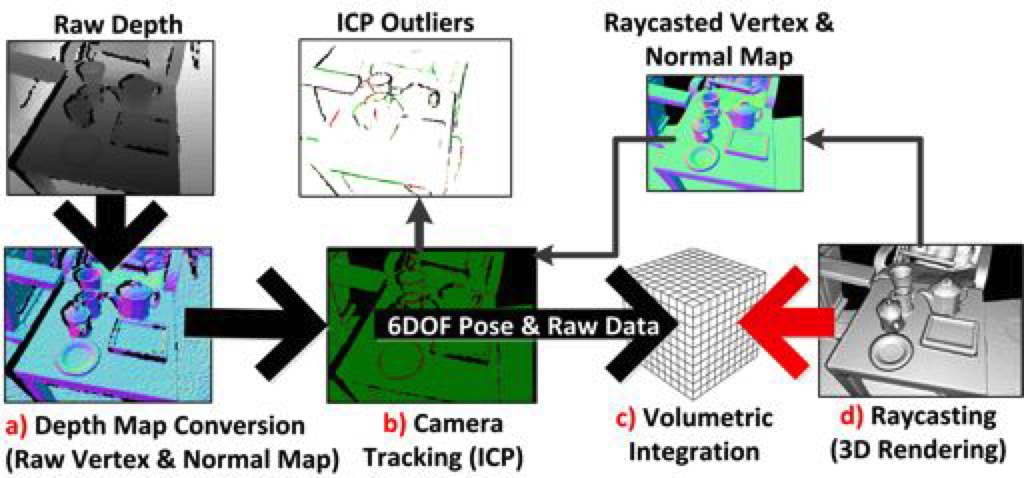
\includegraphics[width=0.7\textwidth]{figures/kinec}
    \caption{Overview of tracking and reconstruction pipeline
from raw depth map to rendered view of 3D scenem\cite{newcombe2011kinectfusion}}
    \label{fig:kinec}
\end{figure}
\\The structure of KinecFusion is given in Fig \ref{fig:kinec} from original paper. The result of ICP is a transformation matrix from previous camera pose to the current pose, which is later used for converting the coordinates of current vertexes into the global coordinate frame. These coordinate data is then fused into the current model that uses a volumetric representation, as mentioned before. The 3D space is uniform divided into fixed size voxel grid. The geometry of surface is implicitly stores in these voxels by having zero values of Truncated Signed Distance Functions (TSDFs) at the surface, positive value in the front of surface, and negative at the back of it. Also, to improve efficiency and minimise storage usage only a truncated area around the surface is actually stored, thus the name "truncated".\\
\\
When integrating the current vertexes into voxel grid, each voxel is perspective projected back onto the image to calculate the difference between it and the measurement depth of this coordinate. The distance difference is then normalized to maximum TSDF distance and updated using weighted average with   previous value. Similar to the implementation of tracking stage, the integration and update process also make use of GPU parallel processing, each thread is assigned a slice of of grid along the $Z-axis$, and sweep through each voxel by its $(x,y)$ position for processing, as shown in Fig \ref{fig:kin}.\\
\begin{figure}[h]
    \centering
    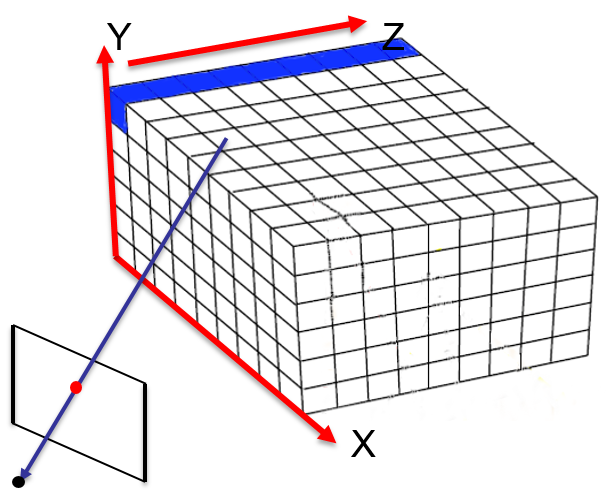
\includegraphics[width=0.5\textwidth]{figures/kin}
    \caption{Volumetric Integration using GPU thread \cite{1_yin_2016}}
    \label{fig:kin}
\end{figure}\\
Finally, in order to render the 3D reconstructed surface raycasting is performed. This is done by having each GPU thread to follow a ray from the camera center along one pixel in the image into the voxel grid in camera coordinate space, the ray is extended until a zero-crossing voxel is met, this voxel represents the surface point observed by this pixel and the position is extracted by doing a trilinear interpolation on this voxel point. And the normal at this position is calculated by find the surface gradent of TSDF values around the position. With these information for each pixel, a live 3D reconstruction view from camera view point can be rendered using camera's pose and intrinsic information.


\subsubsection{Keyframe-Based Visual-Inertial SLAM Using Nonlinear Optimization}
Other than using depth sensor with RGB camera, another kind of sensor equipped on the Google Tango tablet is Inertial Measurement Unit (IMU). Okvis\cite{leutenegger2015keyframe} is a sparse feature-based SLAM approach that tightly coupled IMU measurement with stereo visual measurement using nonlinear optimization.\\
\\
Usually in optimization-based visual SLAM, the structure of geometry is to relate camera poses using landmarks, and optimization is performed to minimize the error of landmark reprojection in different observing frames. However, in visual inertial SLAM, the IMU measurement is used to add additional constraint between camera poses and speed and estimation biases from gyroscopes and accelerometers. The structure graph from original paper is shown in Fig \ref{fig:kinec} with detail labelling of different variables and constraints.\\
\begin{figure}[h]
    \centering
    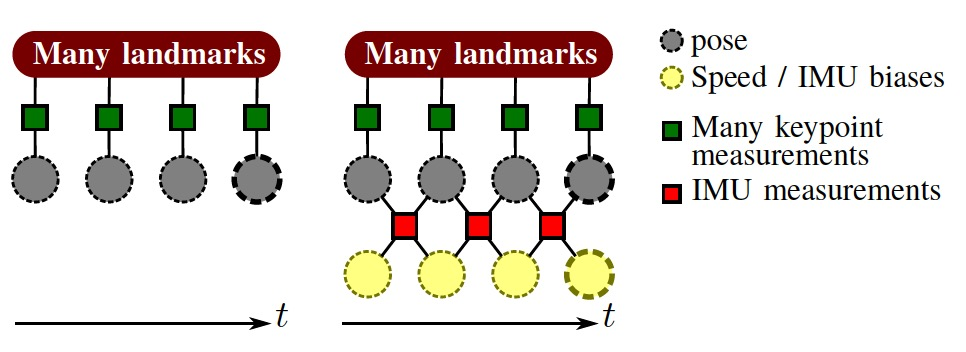
\includegraphics[width=0.7\textwidth]{figures/okvis}
    \caption{graph of variables and their relationships in visual SLAM on the left and visual intertial SLAM on the right \cite{leutenegger2015keyframe}}
    \label{fig:okvis}
\end{figure}\\
In order to tightly couple the visual and inertial measurements, a joint nonlinear cost function that contains both visual reprojection error term and IMU error term is created. These both errors are eliminated by optimizing this one error function.\\
\\
To reduce complexity and ensuring real time operation, a fixed size temporal window of robots poses and relative states is maintained, and old robot poses will be marginalized out as new frames are inserted.\\
In the visual frontend, a sparse map of frames and landmarks is stored. For each new frame, keypoints are extracted using SSE(Streaming SIMD Extensions)-optimized Harris corner detector and BRISK(Binary Robust Invariant Scalable Keypoints) descriptor, their 3D positions are then triangulated by stereo and put into the sparse map. During the process landmarks and keypoints are brute-forcely matched and outliers are rejected by using predicted pose from IMU data. In the optimization window, two kind of frames is maintained, first is a temporal window of the S most recent frames, second is N keyframes in the past. A frame is determined as keyframe if the number of matched points with previous frame is less than 50 to 60\%  of the number of detected keypoints.\\
\\
\begin{figure}[h]
    \centering
    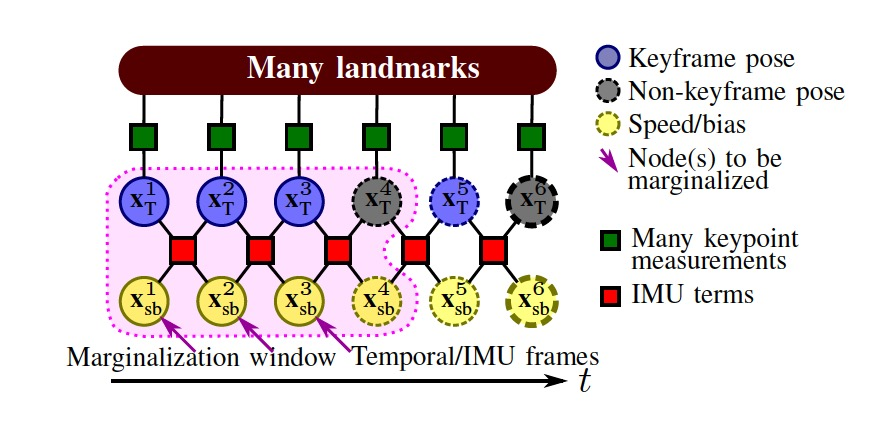
\includegraphics[width=0.7\textwidth]{figures/okvis1}
    \caption{Graph of initial marginalization window \cite{leutenegger2015keyframe}}
    \label{fig:okvis1}
\end{figure}
\begin{figure}[h]
    \centering
    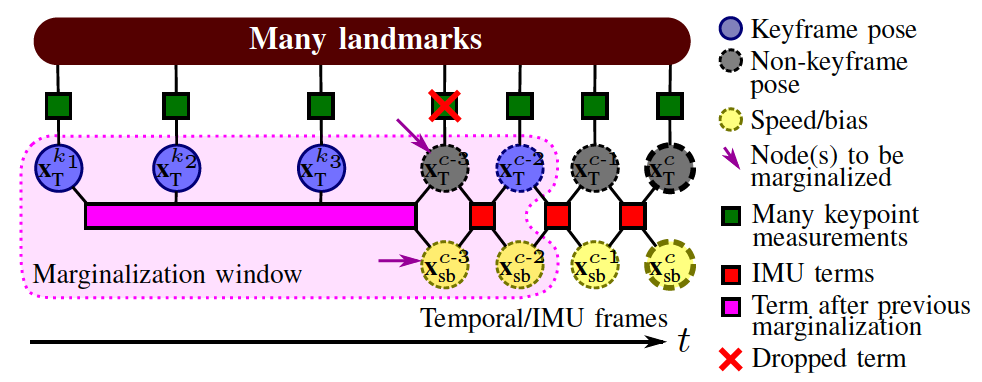
\includegraphics[width=0.7\textwidth]{figures/okvis2}
     \caption{Graph for marginalization in the first case \cite{leutenegger2015keyframe}}
    \label{fig:okvis2}
\end{figure}
\begin{figure}[h]
    \centering
    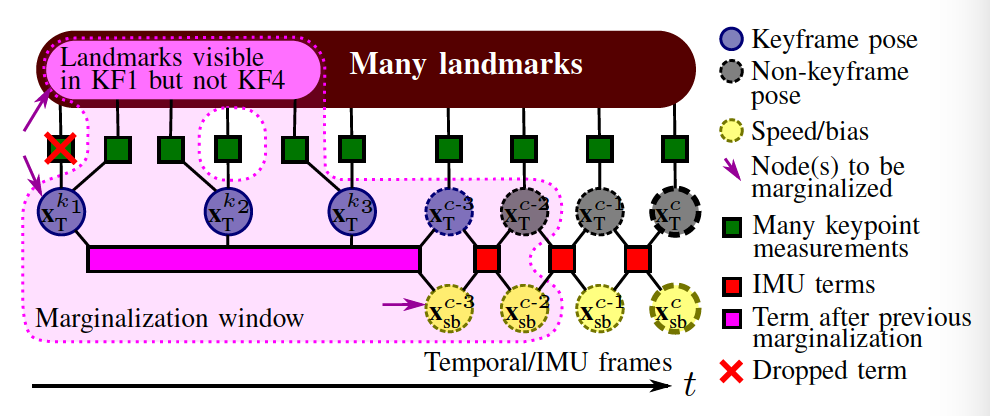
\includegraphics[width=0.7\textwidth]{figures/okvis3}
   \caption{Graph for marginalization in the second case \cite{leutenegger2015keyframe}}
    \label{fig:okvis3}
\end{figure}
In the marginalization process, initially the first $N+1$ frames forms the marginalization window, as shown in Fig \ref{fig:okvis1}. When a new frame is inserted into the marginalization window, there are two ways to marginalize old state. If the oldest frame in temporal window is not a keyframe, then the state of that frame with its measurements, speed and biases will be dropped, as shown in Fig \ref{fig:okvis2}. On the other hand if it is a keyframe, landmarks that are visible in first temporal frame but in most recent keyframe is also dropped, as shown in Fig \ref{fig:okvis3}.\\





\subsubsection{Elasticfusion}
Elasticfusion\cite{whelan2016elasticfusion} is a RGB-D dense SLAM method for 3D reconstruction in room scale without using pose graph  it also use surfels to represent the map instead of voxel grid such as in KinectFusion\cite{newcombe2011kinectfusion}. In the scanning process, it iteratively check for local and global loop closures and refine the map by using a deformation graph to apply non rigid deformation to the surface. However, while this approach has achieved great results in room scale, it may be difficult to be used on bigger or outdoor scenes due to complex light condition and size of memory needed to store the surfels.\\
\\
In the surfel map, each surfel stores the information about a local surface area around the center of the surfel, the surfels are lay out in a wat that holes on the surface are minimised. The information about a surfel include its position, normal vector, color, weight and radius. The radius is larger as distance between image center and surfel is greater. The surfels are extracted from point cloud using the similar method as in \citep{keller2013real}, illustrated in Fig \ref{fig:surfel2}, but differently, in here the surfels are divided into active and inactive parts. Only active surfels are used for camera pose estimation and depth map fusion, while the inactive parts are the surfels that have not been observed for a given time period and can be reactivated in a local loop closure. In ElasticFusion, OpenGL shading language is used to manage the surfel map and update, fuse and render the view. \\
\\
\begin{figure}[h]
    \centering
    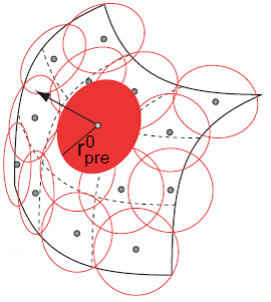
\includegraphics[width=0.5\textwidth]{figures/surfel2}
    \caption{surfel2}
    \label{fig:surfel2}
\end{figure}
The detail structure of ElasticFusion is shown Fig \ref{fig:elas1} in the original paper. From the graph can be seen that firstly in the camera pose estimation step, dense frame-to-model camera tracking is used, geometric and photometric pose estimations are combined into a joint cost function to for minimization. Geometric error is calculated using frame to model projective data association and ICP algorithm as in kinecFusion\citep{newcombe2011kinectfusion}, and photometric error is gain by calculating the intensity difference between current RGB image and backprojected image from the model. Note that here in the tracking process only active surfels are used.\\
\\
\begin{figure}[h]
    \centering
    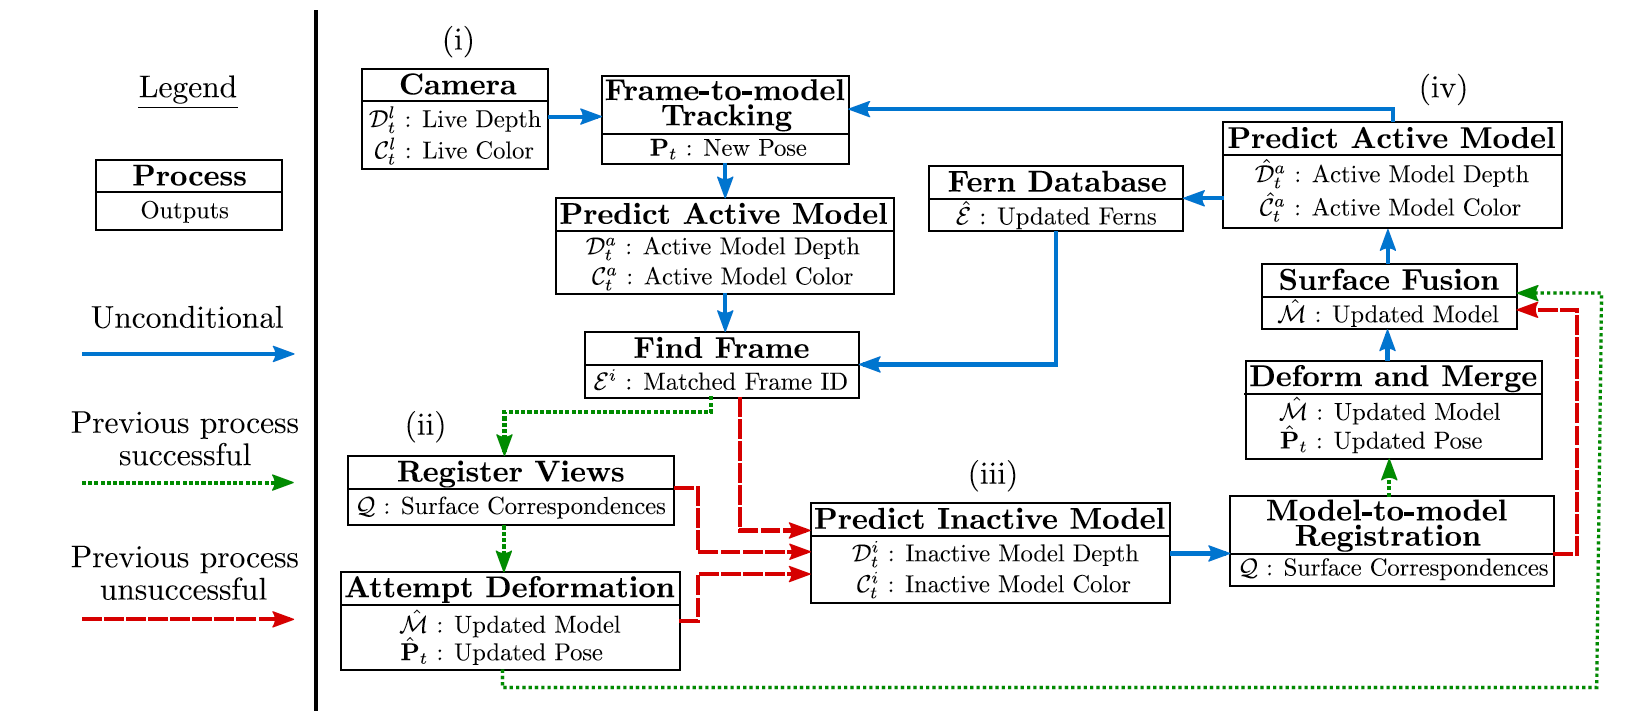
\includegraphics[width=1.0\textwidth]{figures/elas1}
    \caption{elas1}
    \label{fig:elas1}
\end{figure}
After camera pose tracking for each frame, an active predicted model is produced, this model is then rendered into an image for global loop cloure checking, to try recover from drifts produced by accumulating error, and realign the camera pose. To enable global loop closure checking, key frame information from past is stored in a randomized fern encoding database using same technique as in \cite{glocker2015real}, it allows storing and matching frames without putting redundant information into the database. If a high quality match between the current predicted view of active model and a frame in fern database is found, points are sampled from matched frame and active view to construct surface constraints that are used to register the surface together and optimize the deformation graph. Each surface constraint contains a pair of points and timestamps to represent the position of point and the destination position that it should reach the destination after deformation.\\
\\
If no global loop closure is found then local model to model loop closure is checked by try to register the currently predicted inactive model with active model under the current frame, similar method is used when high quality alignment is found, constraints are extracted and fed into  the deformation graph, then the inactive surfels in this alignment is reactivated to allow for fusion into the map.\\
\\
The realignment of map is done by applying non rigid deformation using a deformation graph. Deformation graph  is constructed each frame for efficiency, with nodes sampled uniformly from the surfels using similar method as in DynamicFusion\citep{newcombe2015dynamicfusion}, this is illustrated in Fig \ref{fig:surfel1} to shown the relation between surfel and deformation graph noded. Each node have a rotation matrix and position vector that represents optimization parameter and neighbourhood of each node forms the edge of the graph. Each surfel has a set of influencing nodes that affects the deformation of that surfel.\\
\\
\begin{figure}[h]
    \centering
    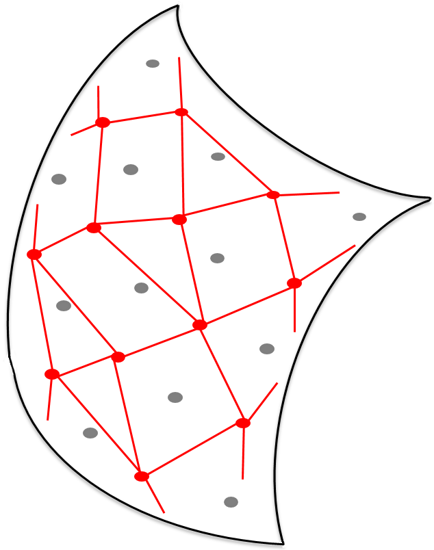
\includegraphics[width=0.5\textwidth]{figures/surfel1}
    \caption{surfel1}
    \label{fig:surfel1}
\end{figure}
The optimization of deformation of the model is done by minimising five cost function in total using the surface constraints constructed in the steps described above. The parameters in surface constraints after optimization reflects the surface registration happened in loop closure. These five cost functions include the following functions: maximises the rigidity of deformation, guarantees the smoothness of deformation in the graph between neighbour nodes, minimises the error in position constraints, that is reduce the difference between source and destination position, also "pins" the inactive surface of the model without moving to make sure is the active surface that deforms into the inactive surface. In the global loop closure optimization process an extra cost function is added, it introduce the set of relative constraints to prevent the previous surface registrations from being pulled apart by subsequent global loop closures. The optimization problem is  solved using iterative Gauss-Newton algorithm on CPU and the result gives a relative transformation matrix that bring the surfaces registered into alignment. The graph Fig \ref{fig:loopclosure} from the original paper have shown the process of a scanning with loop closure happens when the scanning camera revisits area that has been scanned before, with active model coloured by surface normal overlaid on the inactive model in greyscale.\\
\\
After the optimization, deformation graph is applied to the surface by using a weighted distance method to calculate the transformation of each surfel by its influencing nodes. Model is then deformed using this transformation to reflect the registration of surfaces in loop closure. Finally, the current camera data is fused into the latest updated model to update the surfel map under current viewpoint.\\
\\
Before new frame of data come in, the current active model is rendered to an image using the latest predicted pose to prepare for tracking, and also being decided whether this frame will added to the fern database.\\
\begin{figure}[h]
    \centering
    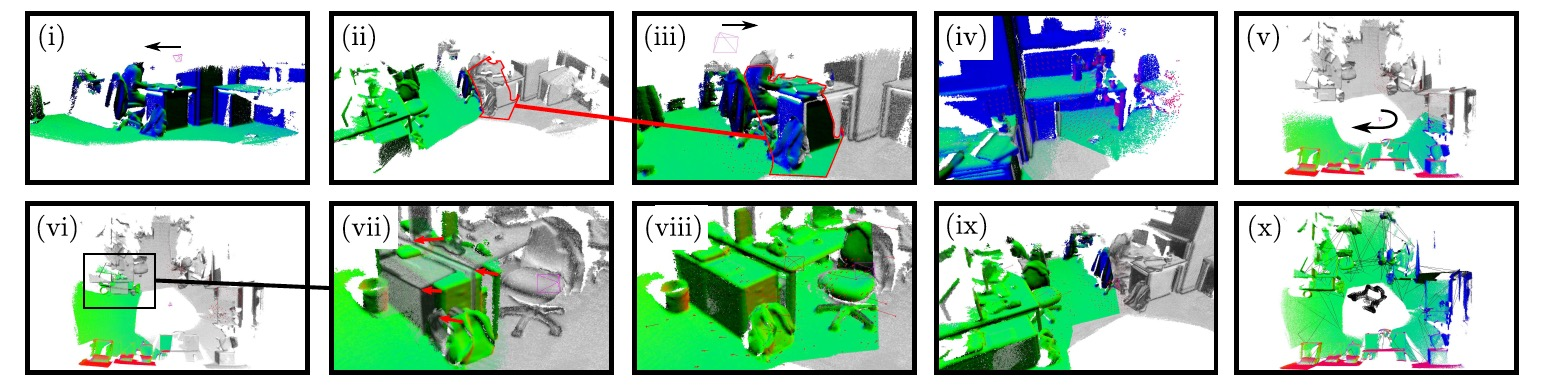
\includegraphics[width=0.7\textwidth]{figures/loopclosure}
    \caption{loopclosure}
    \label{fig:loopclosure}
\end{figure}



\subsection{Related Work}


This section gives some SLAM systems that have been implemented on mobile devices, such as Android phone or tablet, and Apple iPhone or iPad. However, most of these systems mainly focus on the state estimation part of SLAM rather then the mapping part, which means they are not able to be used for 3D surface reconstruction purpose.



\subsubsection{CHISEL}
CHISEL\citep{klingensmith2015chisel} is a large scale dense 3D reconstruction solution implemented on Google Tango Devices. The graph from the original paper that shows CHISEL application running on the Googlt Tango phone can be seen at Fig \ref{fig:CHISEL1}. It uses dynamic spatially-hashed truncated signed distance field\citep{niessner2013real} to represent the map and useds the visual-inertial odometry provided by Tango as frontend for localization. To save memory and computation power, space that does not contain surfaces is culled out. By using space carving, even though Tango's depth sensor provides data with high noise, reconstruction with an accuracy of 2-3 cm is still achieved in large scenes, the Fig \ref{fig:CHISEL2} show a picture of global map reconstructed by CHISEL form the original paper, from this picture can be seen that CHISEL is able to scan and reconstruct the area of a flat with relatively high quality detail. To generalise the solution onto other mobile devices that does not have a powerful GPU,in CHISEL no parallel processing is used to utilise the powerful general purpose GPU provided on Google Tango tablet.\\
\\
In the pose estimation stage, CHISEL uses the pose estimated provided by Tango platform as a black box, by try to register each depth scan with the model, poses are optimised in the same way as using ICP algorithm, this allows small drifts between frames to be recovered, however during long process of scanning large scene, drifts will still build up overtime due to the lack of loop closure process.\\
\\
Since the map is stored using spatially-hashed data structure, insert and look up is very fast. The map is divided into chunks, and each chunk is a fixed grid of voxels. These chunks are then spatially-hashed into a spatial 3D hash map. When looking for chunks that need to be updated or drawn, a camera frustum is created for culling chunks that do not intersect with the frustum or not have a depth data, the rest of chunks left is then processed for update or drawn.\\
\\
For fusing depth scan data into the model, projection mapping is used to compare the depth value on image with the projected visual hull of a voxel, the result is then used to update the TSDF value and weight of that voxel.\\
\\
In the rendering stage, incremental Marching Cubes is used to generate triangle meshes for the chunk when it is been updated by a depth scan, triangles are generated at the zero isosurface of the TSDF volxel grid.\\
CHISEL has shown a nice memory-efficient approach to scanning large scene for high quality 3D reconstruction, however it fails to maintain global consistency of the global map, therefore drifts will increase over time due to lacking detection of global loop closure. Despite that, CHISEL provides a great example for utilising the Tango platform as a dense SLAM frontend for 3D reconstruction purpose.

\begin{figure}[h]
    \centering
    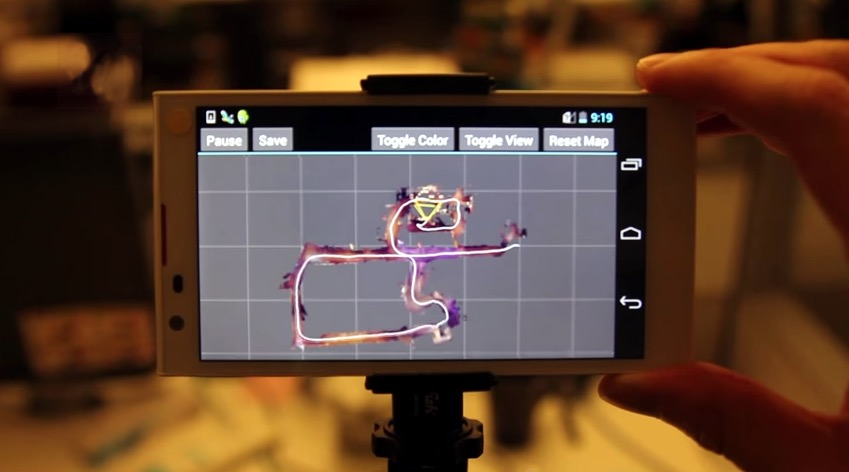
\includegraphics[width=0.7\textwidth]{figures/CHISEL1}
    \caption{CHISEL1}
    \label{fig:CHISEL1}
\end{figure}

\begin{figure}[h]
    \centering
    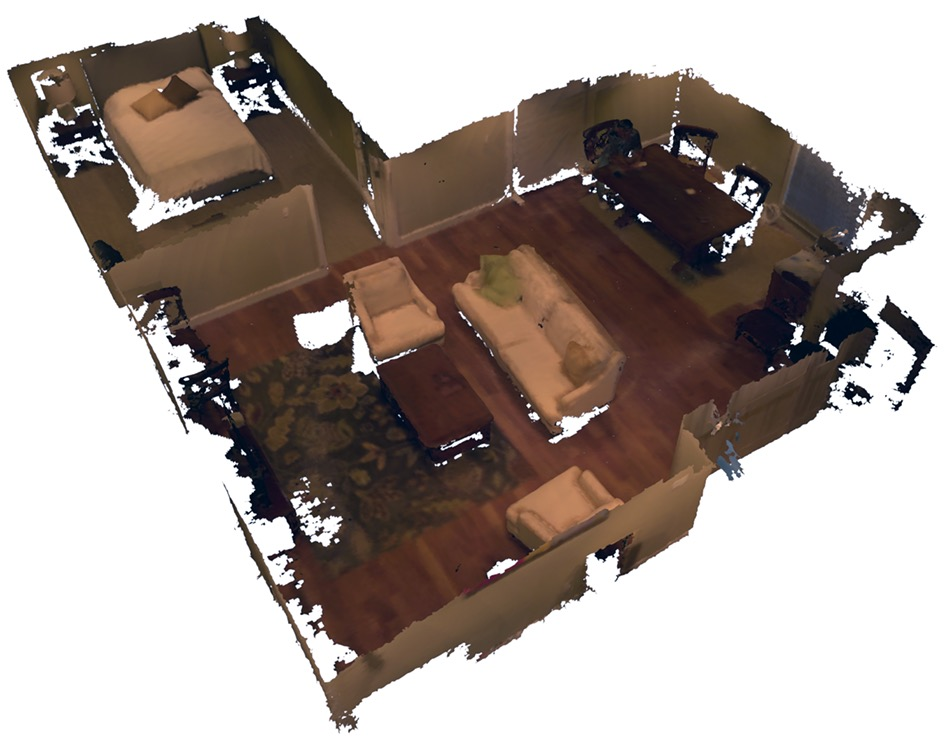
\includegraphics[width=0.7\textwidth]{figures/CHISEL2}
    \caption{CHISEL2}
    \label{fig: CHISEL2}
\end{figure}



\subsubsection{InfiniTAM}
InfiniTAM\citep{InfiniTAM_ISMAR_2015} is an open source cross-platform real time large scale RGB-D SLAM framework publish by University of Oxford\footnote{\url{https://github.com/victorprad/InfiniTAM}}. It provides both dense fixed size 3D volume like the one used in KinectFusion\citep{newcombe2011kinectfusion} and sparse volume using voxel block hashing method\citep{niessner2013real}. The design of the framework also enables other representations, such as octrees, to be added easily.\\
\\
InfiniTAM is optimised to run at high frame rate in multiple platform, with NVIDIA Titan X graphics card on desktop computer, it can run at over 1000 fps(frame per second), on iOS platform it utilise Apple Metal Graphics API to reach over 25 fps of frame rate. Also on Android devices with NVIDIA K1 processor such as NVIDIA Shield Tablet and Google Tango Tablet, by using NVIDIA CUDA to for parallel data processing on GPU the frame rate is able to reach over 40 fps.\\
\\
The architecture designed for InfiniTAM makes it easy to extend functionalities and add new features. Also the C++ source code for InfiniTAM is provided on Github for both pure CPU and GPU implementations. The Android version of InfiniTAM is similar to ElasticFusion since it also use both OpenGL and CUDA in the program, it has provided an example of dense 3D reconstruction solution on mobile device using volumetric space representation and CUDA for GPU acceleration. The sample screen shot of using InfiniTAM from the official website is given below at Fig \ref{fig: InfiniTAM}.\\

\begin{figure}[h]
    \centering
    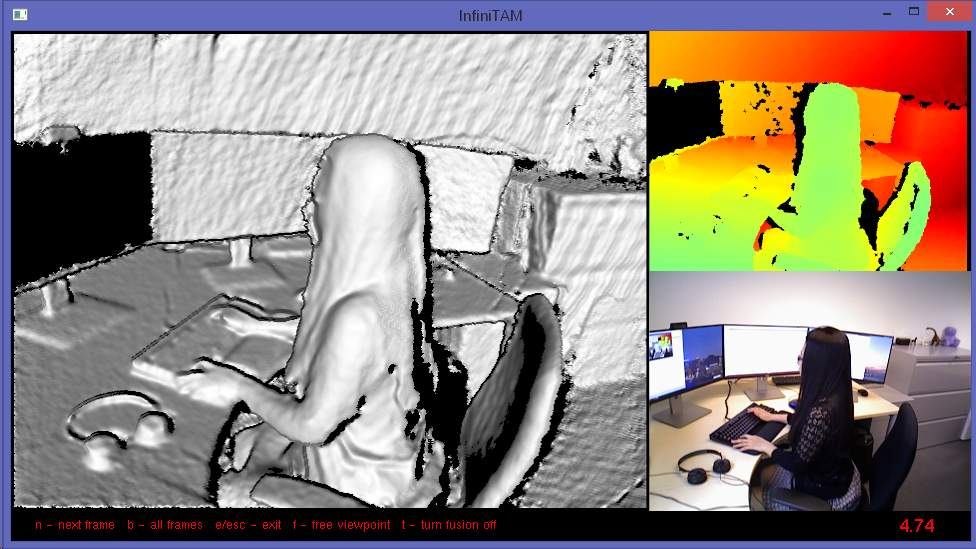
\includegraphics[width=0.7\textwidth]{figures/InfiniTAM}
    \caption{InfiniTAM}
    \label{fig: InfiniTAM}
\end{figure}

\begin{figure}[h]
    \centering
    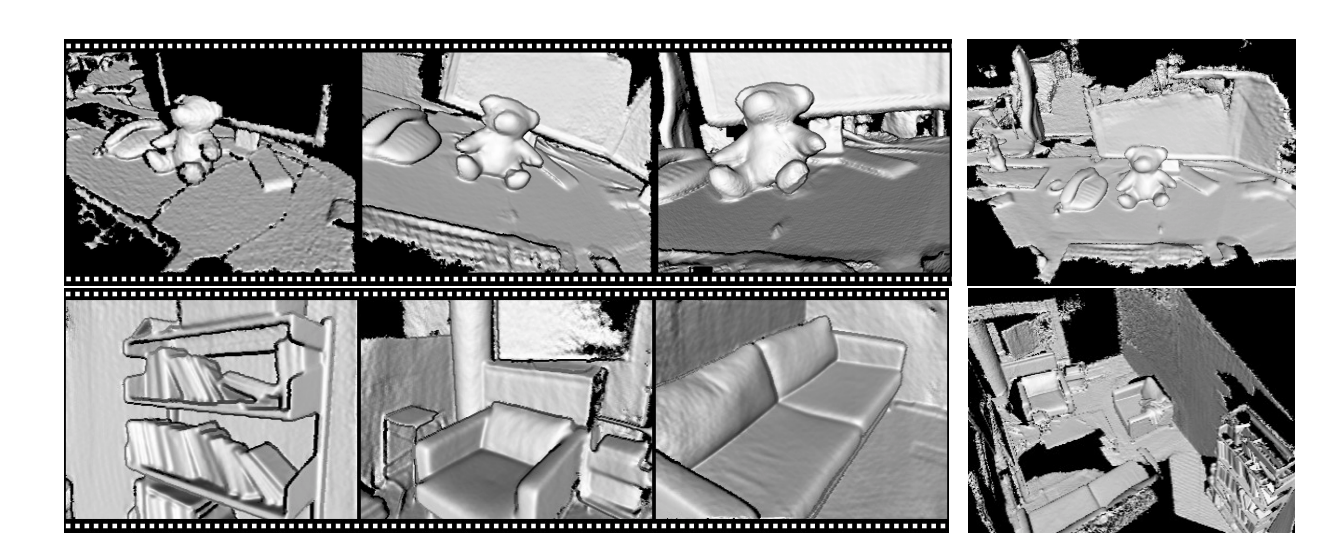
\includegraphics[width=0.7\textwidth]{figures/InfiniTAM2}
    \caption{InfiniTAM2}
    \label{fig: InfiniTAM2}
\end{figure}


\subsubsection{ORB-SLAM on mobile devices}
ORB-SLAM is a monocular real time SLAM system based on detecting feature points of input image, with loop closure detection and camera relocalization function. It's capable of being used in both indoor and outdoor scenes at various scales, and its localization stays robust even with rapid motion of camera.\\
\\
ORB-SLAM2\citep{mur2016orb}\footnote{\url{https://github.com/raulmur/ORB_SLAM2}} is an open source system builds on previous work of ORB-SLAM, supports not only monocular but also stereo and RGB-D cameras used for computing camera trajectory and sparse 3D reconstruction with true scale.\\
\\
ORB-SLAM system is divided into three thread performing different functions, the tracking thread is responsible for extracting key points from the input image, as shown in picture Fig \ref{fig: orb1} from the original paper, this is done by using ORB descriptors, which later are used for pose estimation from the last frame and then decide whether this is a new key frame. the LocalMapping thread inserts the key frame and create map points to perform a local BA(Bundle Adjustment) for optimization, and it maintains a covisibility graph for keypoint and pose tracking. Lastly the LoopClosing thread detects loop closure using Bag-of-words method\citep{galvez2012bags}, and perform loop correction by optimising a essential graph if loop closure is detected. With loop closure detection, as shown in the picture Fig \ref{fig: orb2} from original paper, ORB-SLAM is able to compute camera trajectory consist with the world and reconstruct a sparse map of the world in accurate alignment even in large outdoor scenes.\\
\\
Since ORB-SLAM2 is a robust SLAM system with robust tracking and loop closure function, there has been many work to implement it on mobile devices using its open source code. Here a few of these work that is open sourced on Github is listed with its dependencies used.
\begin{itemize}
   \item \verb|ORB_SLAM2_Android|\footnote{\url{https://github.com/FangGet/ORB_SLAM2_Android}} ported ORGB-SLAM2 on Android, using DBoW2\footnote{\url{https://github.com/dorian3d/DBoW2}} for loop detection, clapack\footnote{\url{http://www.netlib.org/clapack/}} and eigen3\footnote{\url{http://eigen.tuxfamily.org/index.php?title=3.0}} for math calculation, and g2o\footnote{\url{https://github.com/RainerKuemmerle/g2o}} for graph optimization and OpenCV for Android. Pangolin\footnote{\url{https://github.com/stevenlovegrove/Pangolin}} was in the original open source code for visualization and user interface and is removed in this implementation.
   \item \verb|ORB-SLAM-Android|\footnote{\url{https://github.com/castoryan/ORB-SLAM-Android}} is also an implementation of ORB-SLAM on Android using DBoW2 and g2o.
   \item \verb|ORB_SLAM_iOS|\footnote{\url{https://github.com/egoist-sx/ORB_SLAM_iOS}} is implemented on iOS platform with dependencies ported in the same way.
  \end{itemize}
\begin{figure}[h]
    \centering
    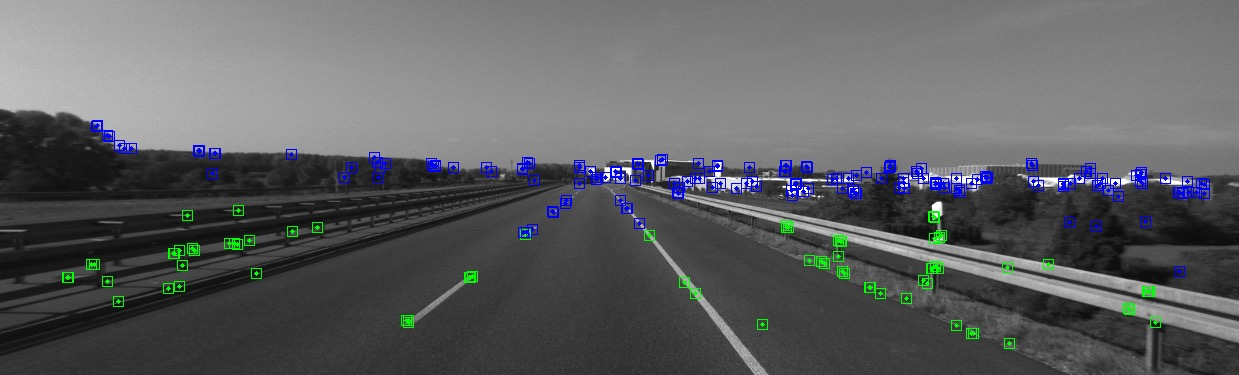
\includegraphics[width=0.7\textwidth]{figures/orb1}
    \caption{orb1}
    \label{fig: orb1}
\end{figure}

\begin{figure}[h]
    \centering
    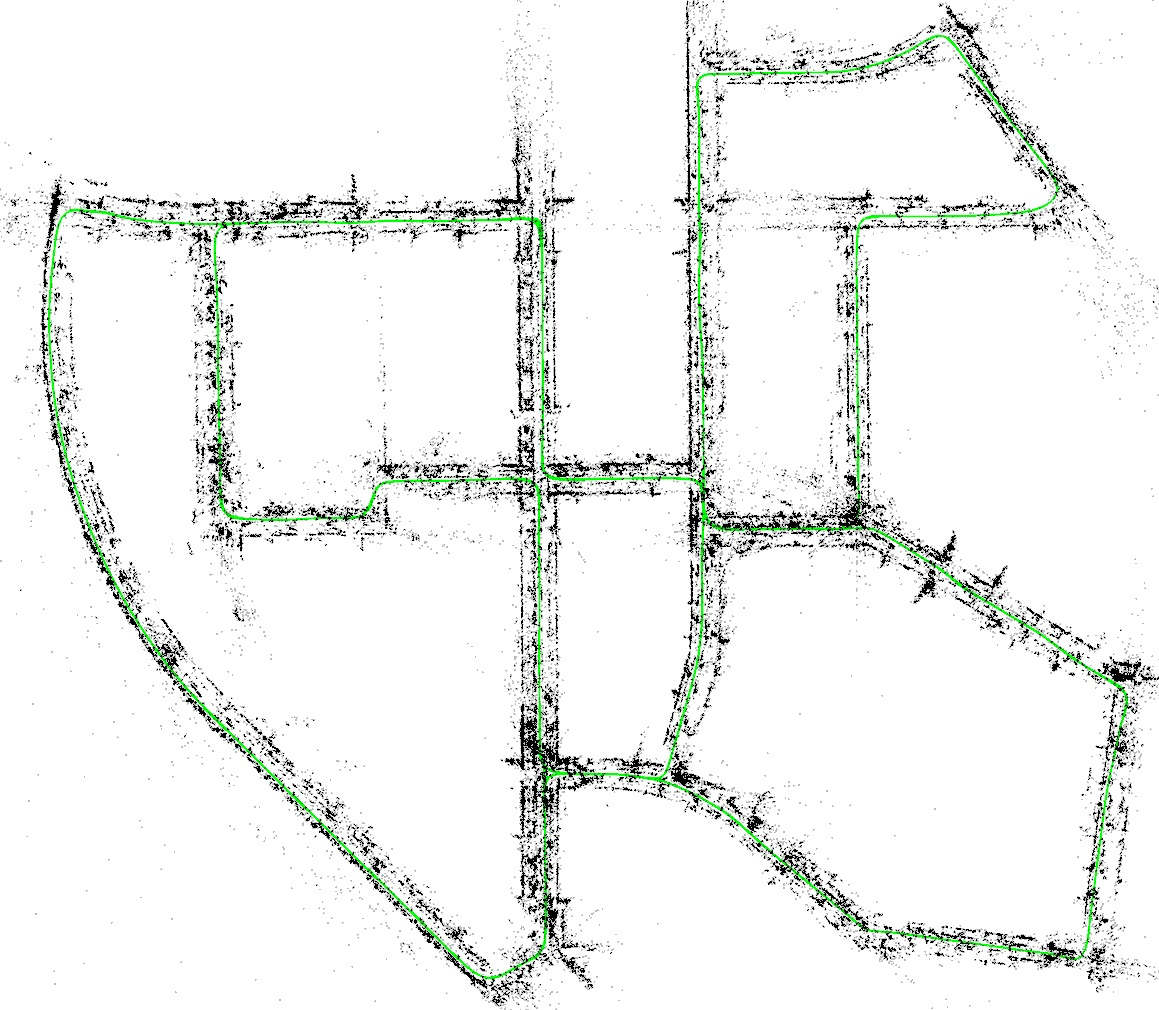
\includegraphics[width=0.7\textwidth]{figures/orb2}
    \caption{orb2}
    \label{fig: orb2}
\end{figure}


\subsubsection{LSD SLAM}
LSD-SLAM(Large-Scale Direct Monocular SLAM)\citep{engel2014lsd}\footnote{\url{https://github.com/tum-vision/lsd_slam}} is a real time direct monocular SLAM system. It uses pixel intensities of input image to track the pose directly, the alignment two images is done by minimising photometric error using Gauss-Newton algorithm. And depth map is estimated using extended Kalman filter (EKF), a $Sim(3)$ pose-graph of keyframes is maintained to allow for loop closure, using g2o library to optimize the pose graph, this corrects drift occur during the process. As the result, a semi-dense 3D map of point clouds is reconstructed in high accuracy. The structure of LSD-SLAM is shown in Fig \ref{fig: lsdslam1} using the graph from original paper.\\
\\
LSD-SLAM not only runs a desktop CPU in real time, it can also run on a modern smartphone for AR application without any GPU acceleration. In this paper \citep{schops2014semi}, an AR application is built on top of direct semi-dense visual odometry using LSD SLAM. In this experiment the application runs on Sony Xperia Z1 smartphone with Android platform, real time performance of at least 30 fps frame rate is reached makes it  capable of used as interactive application, this is due to the separation of tracking and mapping part in the application, and also using NEON optimization for computational heavy parts. The structure of application is shown in Fig \ref{fig: lsdar2}, also Fig \ref{fig: lsdar1} shows the virtual object added in AR application, depth map estimated from the current image and collision mesh created for virtual object to interact with. Both pictures are from the original paper.

\begin{figure}[h]
    \centering
    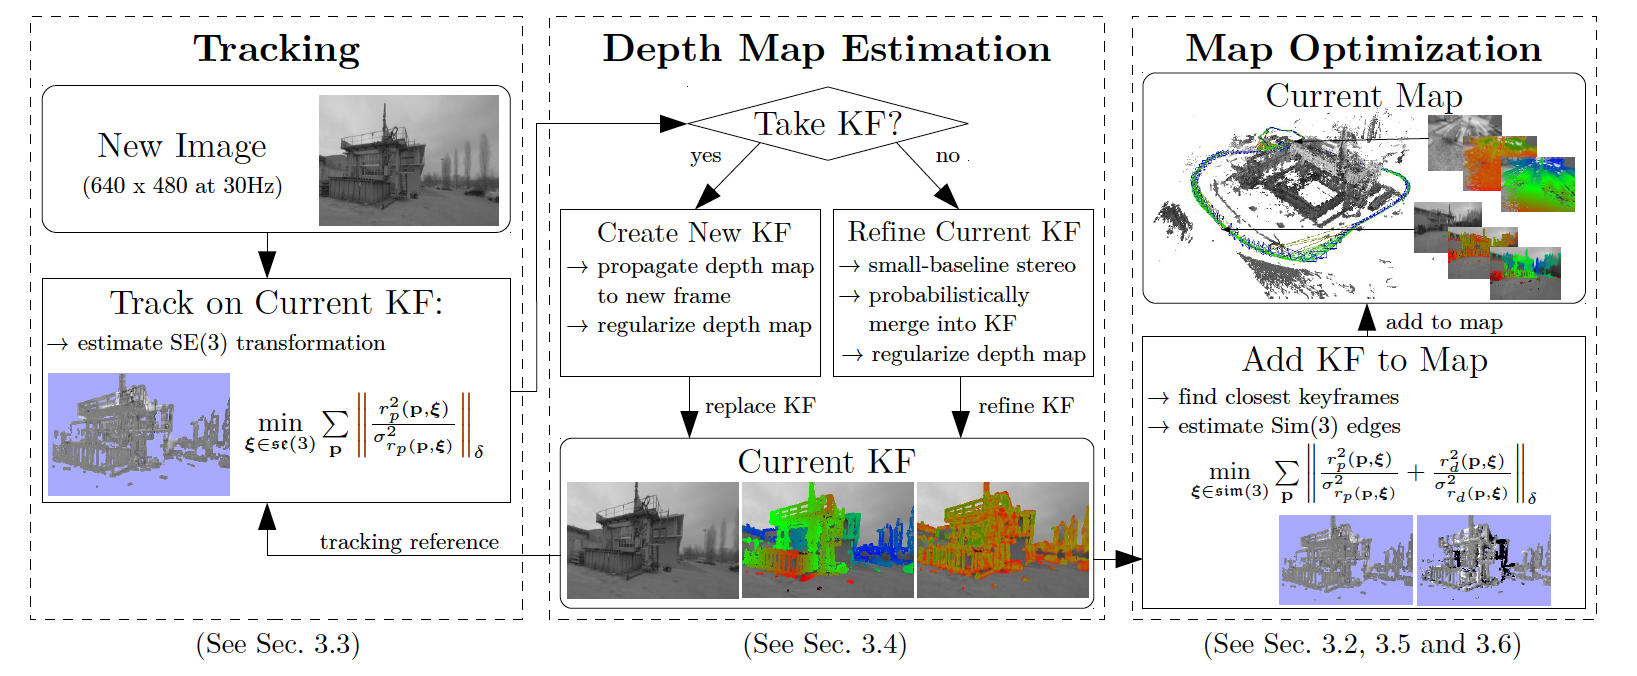
\includegraphics[width=1.0\textwidth]{figures/lsdslam1}
    \caption{lsdslam1}
    \label{fig: lsdslam1}
\end{figure}

\begin{figure}[h]
    \centering
    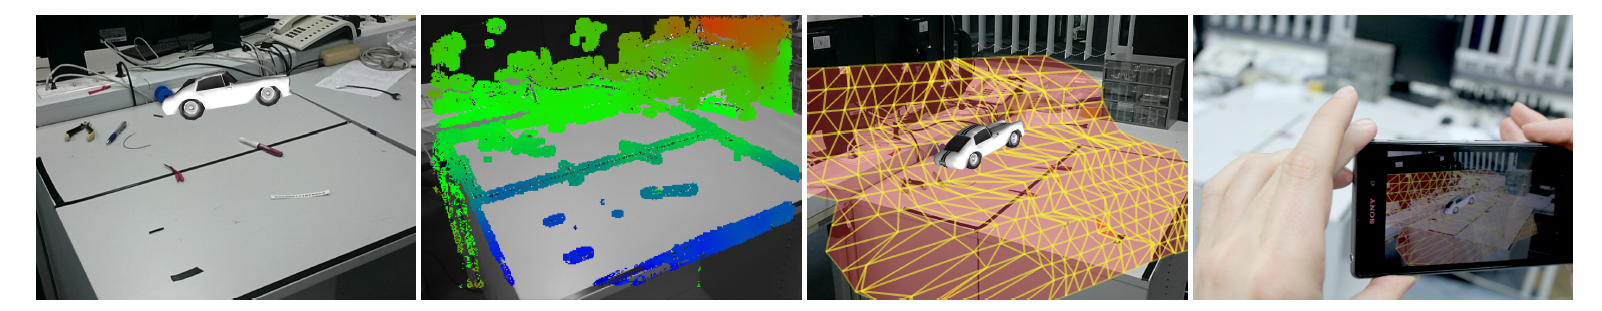
\includegraphics[width=0.7\textwidth]{figures/lsdar1}
    \caption{lsdar1}
    \label{fig: lsdar1}
\end{figure}

\begin{figure}[h]
    \centering
    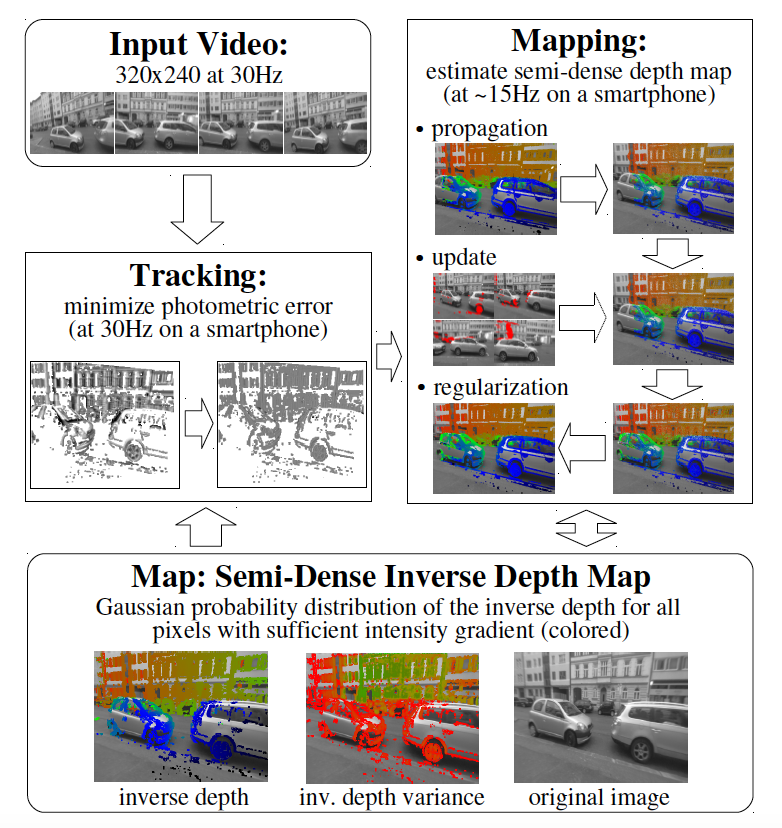
\includegraphics[width=0.7\textwidth]{figures/lsdar2}
    \caption{lsdar2}
    \label{fig: lsdar2}
\end{figure}


\subsubsection{VINS-Mobile}
VINS-Mobile\citep{yang2017monocular} is a open source\footnote{\url{https://github.com/HKUST-Aerial-Robotics/VINS-Mobile}} real time Monocular Visual-Inertial State Estimator on mobile devices developed by members in HKUST Aerial Robotics Group. It can run on iOS devices for providing localization function in AR (augmented reality) applications and also on UAV (Unmanned aerial vehicle) for state estimation.\\
\\
It provides highly accurate visual-inertial odometry by using sliding window optimization, and also enables automatic initialization, relocalisation and loop closure function. The drift error accumulated over time is corrected by optimise the global pose graph maintained. In this picture Fig \ref{fig: vin1} from the paper \footnote{\url{http://www.ece.ust.hk/~eeshaojie/ismar2017peiliang.pdf}} can be seen that the virtual object added in the AR application remains in place even after the camera have travelled a long loopy trajectory.\\
\\
The program uses ceres solver\citep{ceres-solver} from Google\footnote{\url{https://github.com/ceres-solver/ceres-solver}} for non-linear optimization in state estimation stage, the loop closure function is implemented using bag of words method DBoW2\footnote{\url{https://github.com/dorian3d/DBoW2}} similar to ORB-SLAM's loop detection function. The screenshot of AR application is shown in Fig \ref{fig: vin2} and the structure of the application is shown in Fig \ref{fig: vin3}. Both pictures are from the original paper.\\

\begin{figure}[h]
    \centering
    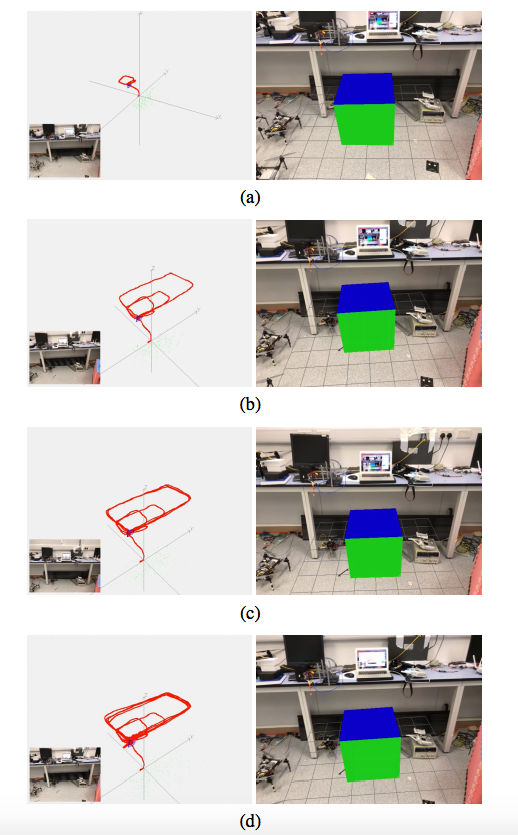
\includegraphics[width=0.7\textwidth]{figures/vin1}
    \caption{vin1}
    \label{fig: vin1}
\end{figure}

\begin{figure}[h]
    \centering
    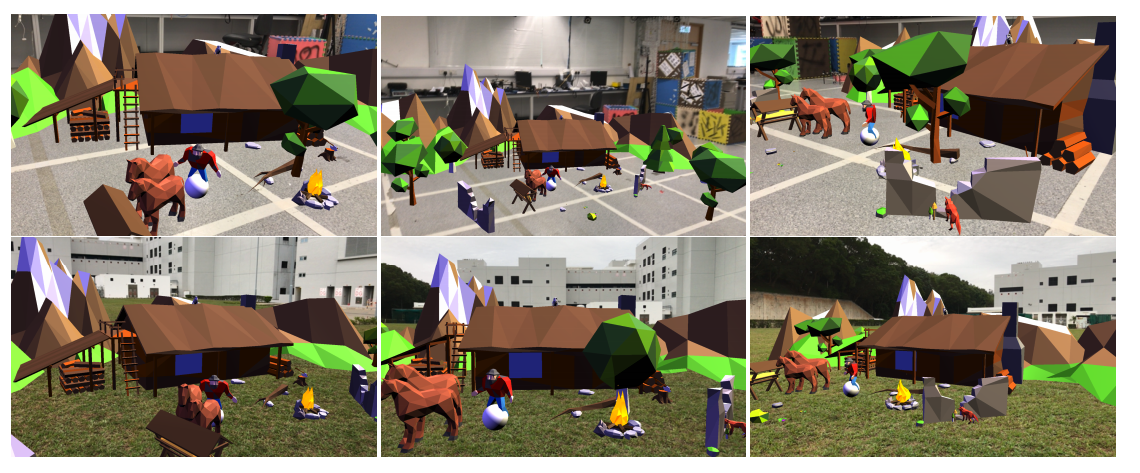
\includegraphics[width=0.7\textwidth]{figures/vin2}
    \caption{vin2}
    \label{fig: vin2}
\end{figure}


\begin{figure}[h]
    \centering
    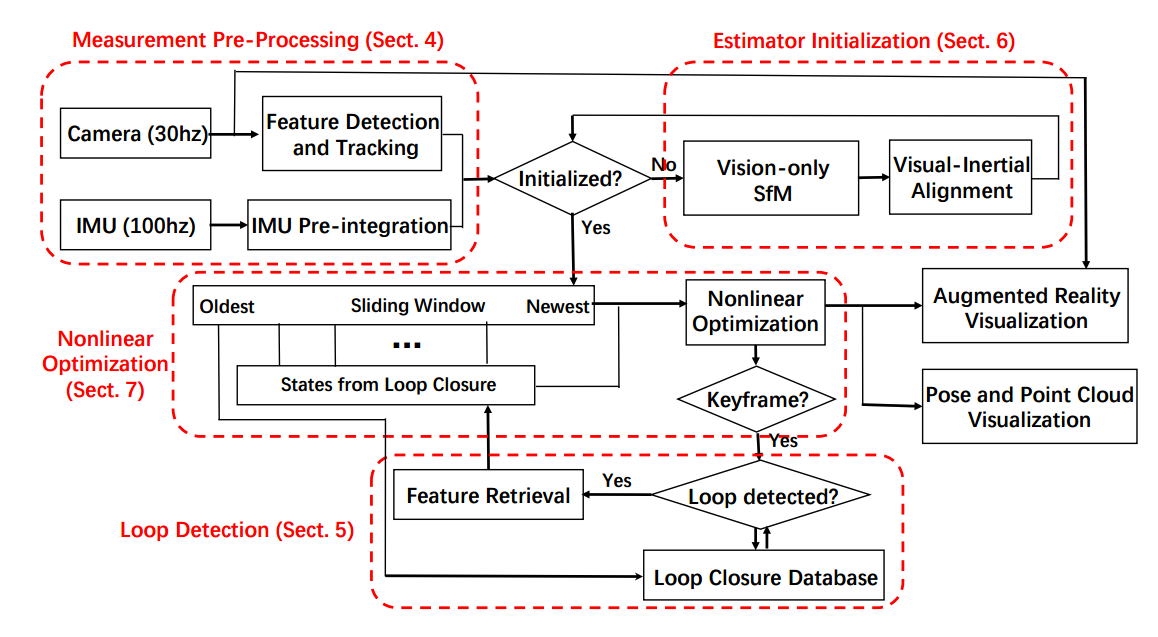
\includegraphics[width=0.9\textwidth]{figures/vin3}
    \caption{vin3}
    \label{fig: vin3}
\end{figure}

\newpage


\section{Project Method Overview}
This project develops an Android application running on the Google Tango \citep{tango} tablet that can either logs RGB, depth and pose data from Tango to files, or run ElasticFusion on tablet using data from Tango platform, or run ElasticFusion using data from dataset on the tablet.\\
\\
The application starts with sample Tango demo applications from Google that uses Tango C API, the code for these applications are most written in C++ under the Java NDK(Native Development Kit) on Android platform, which allows it to use the Tango Client C API, the source code for these demo applications can be found on Github\footnote{\url{https://github.com/googlesamples/tango-examples-c}}.\\
\\
One demo application that is useful for this project is the RGB depth sync application\footnote{\url{https://github.com/googlesamples/tango-examples-c/tree/master}}, it make use of both Tango's Motion Tracking and Depth Perception feature. And it calculates a depth map by use an upsample method to match the Tango Point Cloud data with each pixel in the RGB image from color camera, and it renders the RGB image on screen with an overlay of grey scale depth map that can adjust the alpha value. The  screen shot of only RGB image rendered is shown in Fig \ref{fig: rgbd3}, and the screen shot with the depth map overlay set to about 0.5 is shown in Fig \ref{fig: rgbd5}, also screen shot of only depth map rendered(alpha value of 1) is shown in
Fig \ref{fig: rgbd6}.\\
\\
The application developed in this project make use of the code for Advanced Estimation in Robotics (433H) course practical exercise as the basic frame work, it's also an Android application running on the Google Tango tablet. On top of this application, first using the Tango Client C API the RGB image data, Tango Point Cloud data, and Tango Pose data is acquired. The RGB image data from camera is gain as the RGB color value of each pixel, and the Tango Point Cloud data is in the form of an array of 3D point coordinates, where each 3D point represent a pixel in the depth image where depth sensor has a reading. And the Pose data comes in as the latest pose estimated by Tango VIO(Visual Inertial Odometry) frontend using the IMU onboard and mono image from wide angle motion tracking camera, details of technique used in the Tango VIO can be found in \cite{mourikis2007multi} and \cite{kottas2013consistency}, but in this project it is treated as a black box.\\
\\
After the Tango Point Cloud Data is acquired, it needs to be process in the same way as in the Tango demo application RGB depth sync, each depth value of 3D point in Tango Point Cloud is upsampled at a window around the point to produce a depth map that is matched with the RGB image.\\
Then according to which function the user of application choose to run, these data of a frame is stored into a circular buffer of fixed size for use by another thread. If the user choose to log these RGBD and pose data into files, the data logging thread takes the latest frame of data put that was stored in the buffer, and then the depth buffer is compressed using the \textit{compress2} function from zlib library\footnote{\url{http://zlib.net/
}}. The RGB image data is also compressed into JPEG format using OpenCV library for Android\footnote{\url{http://opencv.org/platforms/android/}}. After that the RGBD and pose data is written to two files respectively, for later use such as using as dataset for running ElaticFusion on desktop computing.\\
\\
The main purpose of this project is allow ElasticFusion run on the Tango tablet for 3D reconstruction with data from Tango as input, therefore the code for ElasticFusion on desktop is ported and adapted to run on Android under NDK environment. The source code of ElasticFusion is available on Github\footnote{\url{https://github.com/mp3guy/ElasticFusion}}, however in this project an internal version of source code is used. The source code of ElasticFusion included three parts: the Core part contains the code for ElasticFusion algorithm, and can be used as an API for other application, the GIU part is responsible the displaying the user interface of program and handles input setting from the command line, reading from files provided for the program, the there is a GPUTest program that user can test the performance of their GPU for running ElasticFusion.\\
In this project, only the core part of ElasticFusion is used, the original dependency of Pangolin is removed and replaced with plain OpenGL ES code that full fills the same function, other necessary change is made to enable the ElasticFusion program be run on Android platform. When the user starts ElasticFusion on the Tango tablet, a new ElasticFusion thread is started and it takes RGBD and pose data from the circular buffer previously mentioned, and use these frame data as the input to the program.\\
Since ElasticFusion program original required high configuration of hardware on desktop, with the processing power on Tango that is much lower than high end desktop computer, all the features of ElasticFusion that requires more processing are turned off on the Tango to make it run faster, such as disabling $\mathfrak{so}(3)$ pre-alignment, use single level tracking pyramid by enabling fast odometry, and disable loop closure detection.\\
After the user using the device to complete the scanning, the 3D reconstruced surface of the map can be saved into a ply file on the tango tablet, and the saved map can then be viewed using mesh viewing application on the device itself.\\
Other than running ElasticFusion with data from the Tango tablet, in this project for experimentation purpose the application is also able to use dataset placed on the tablet to run ElasticFusion program, a RGBD data file with pre-specified file name has to be on the tablet before that, and a Pose data file is optional, if the pose data is provided, ElasticFusion will be run using the input pose without using the camera tracking process.\\
\\
Originally, in the design of this project, the Android application developed is supposed to render the 3D reconstructed surface on the screen in real time, and augmented reality application can be built on it if the implementation of ElasticFusion on Tango tablet is successful and performance is good enough for interactive application(runs at frame rate higher than 30 Hz). However, during the progress of this project, it is found that ElasticFusion runs poorly and very slowly on the Tango tablet, this is due to the data quality from depth sensor
is not very good and also the processing power on the tablet is much less than what ElasticFusion requires, also partly caused by the time and effort limitation, the 3D reconstructed surface by the application on Tango tablet is still not 100 percent correct, and there was no enough time before project deadline for doing optimization of the application.\\
\\
However, other this Android application developed, in this project a simple way of running ElasticFusion in close loop mode using input pose is created to allow for the input pose to be corrected so that the current pose stored in the ElasticFusion is consistent with the input pose, and no camera tracking step is need thus processing time and power is saved. The change of applying this method is implemented both in the application on Tango tablet and the desktop version of ElasticFusion.\\
The overall structure of the Android application developed in this project is shown in graph Fig \ref{fig: projectStructure}, the graph clearly shown three different thread used for different functions and the frontend-backend structure of the SLAM system developed in this application.\\
\\
\begin{figure}[h]
    \centering
    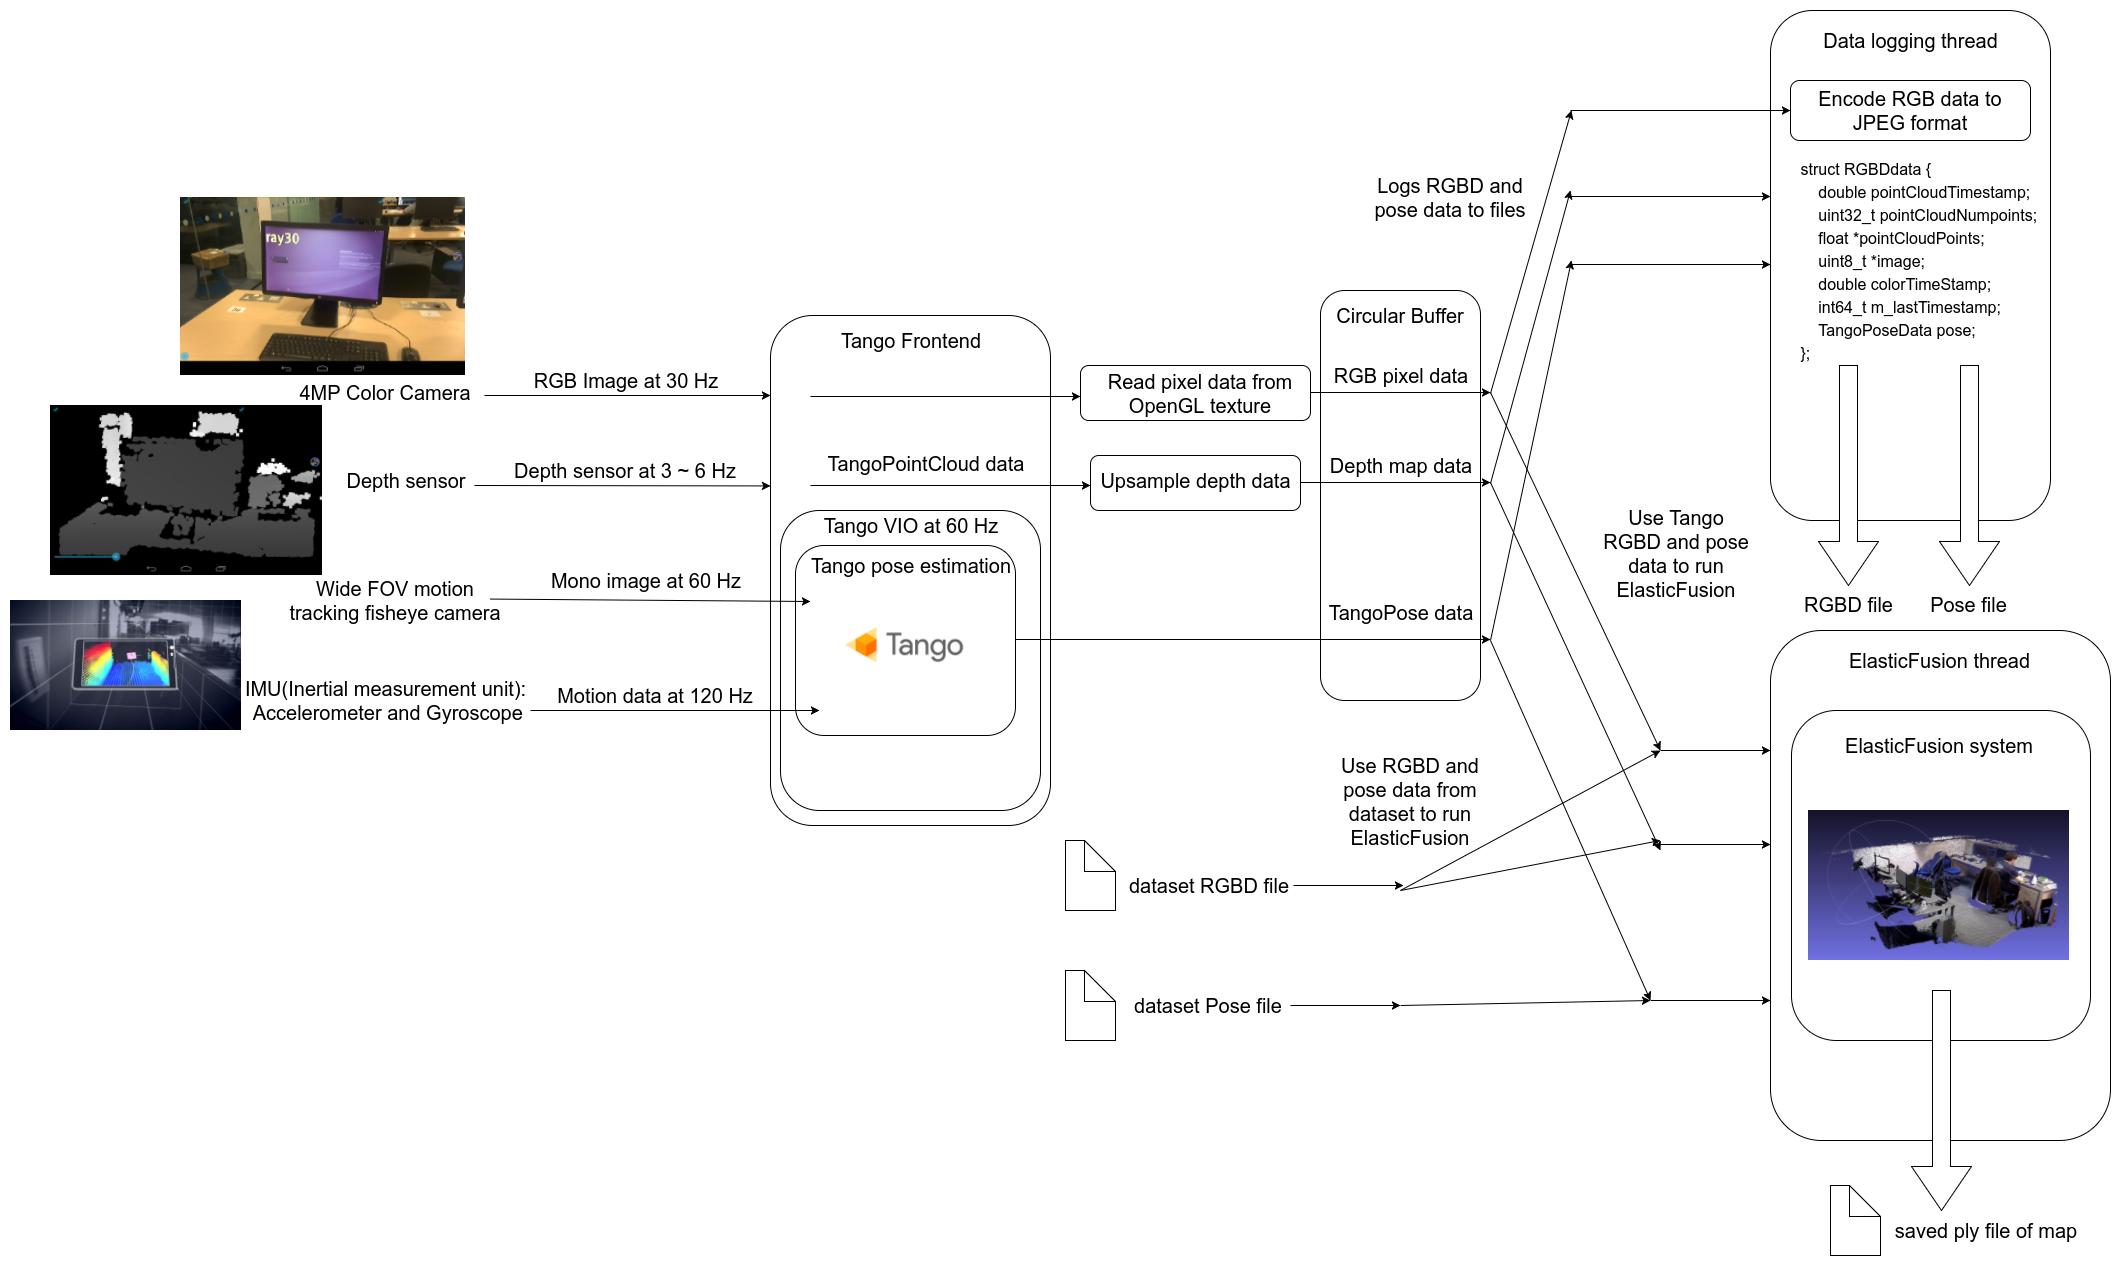
\includegraphics[width=1.0\textwidth]{figures/projectStructure}
    \caption{projectStructure}
    \label{fig: projectStructure}
\end{figure}

\begin{figure}[h]
    \centering
    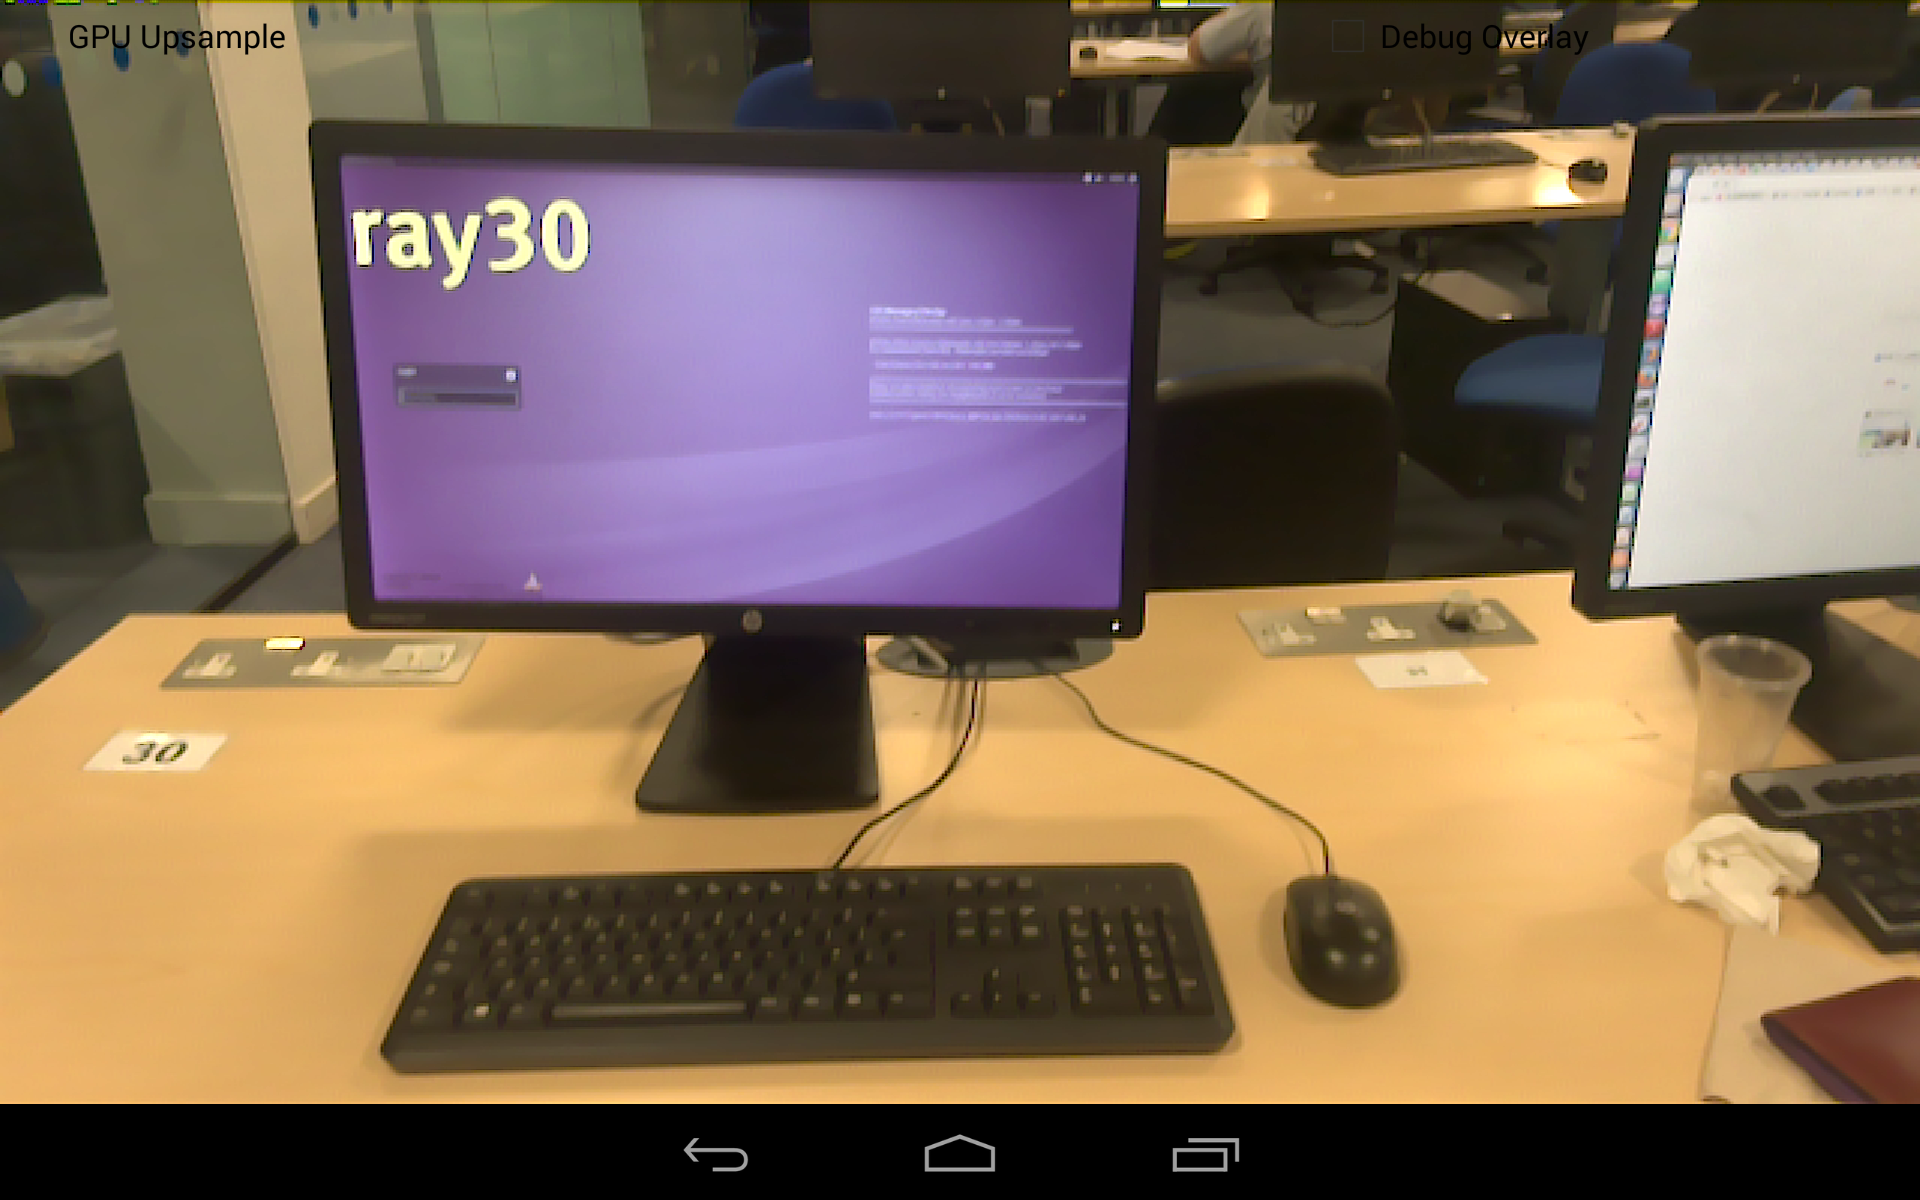
\includegraphics[width=0.7\textwidth]{figures/rgbd1}
    \caption{rgbd1}
    \label{fig: rgbd1}
\end{figure}

\begin{figure}[h]
    \centering
    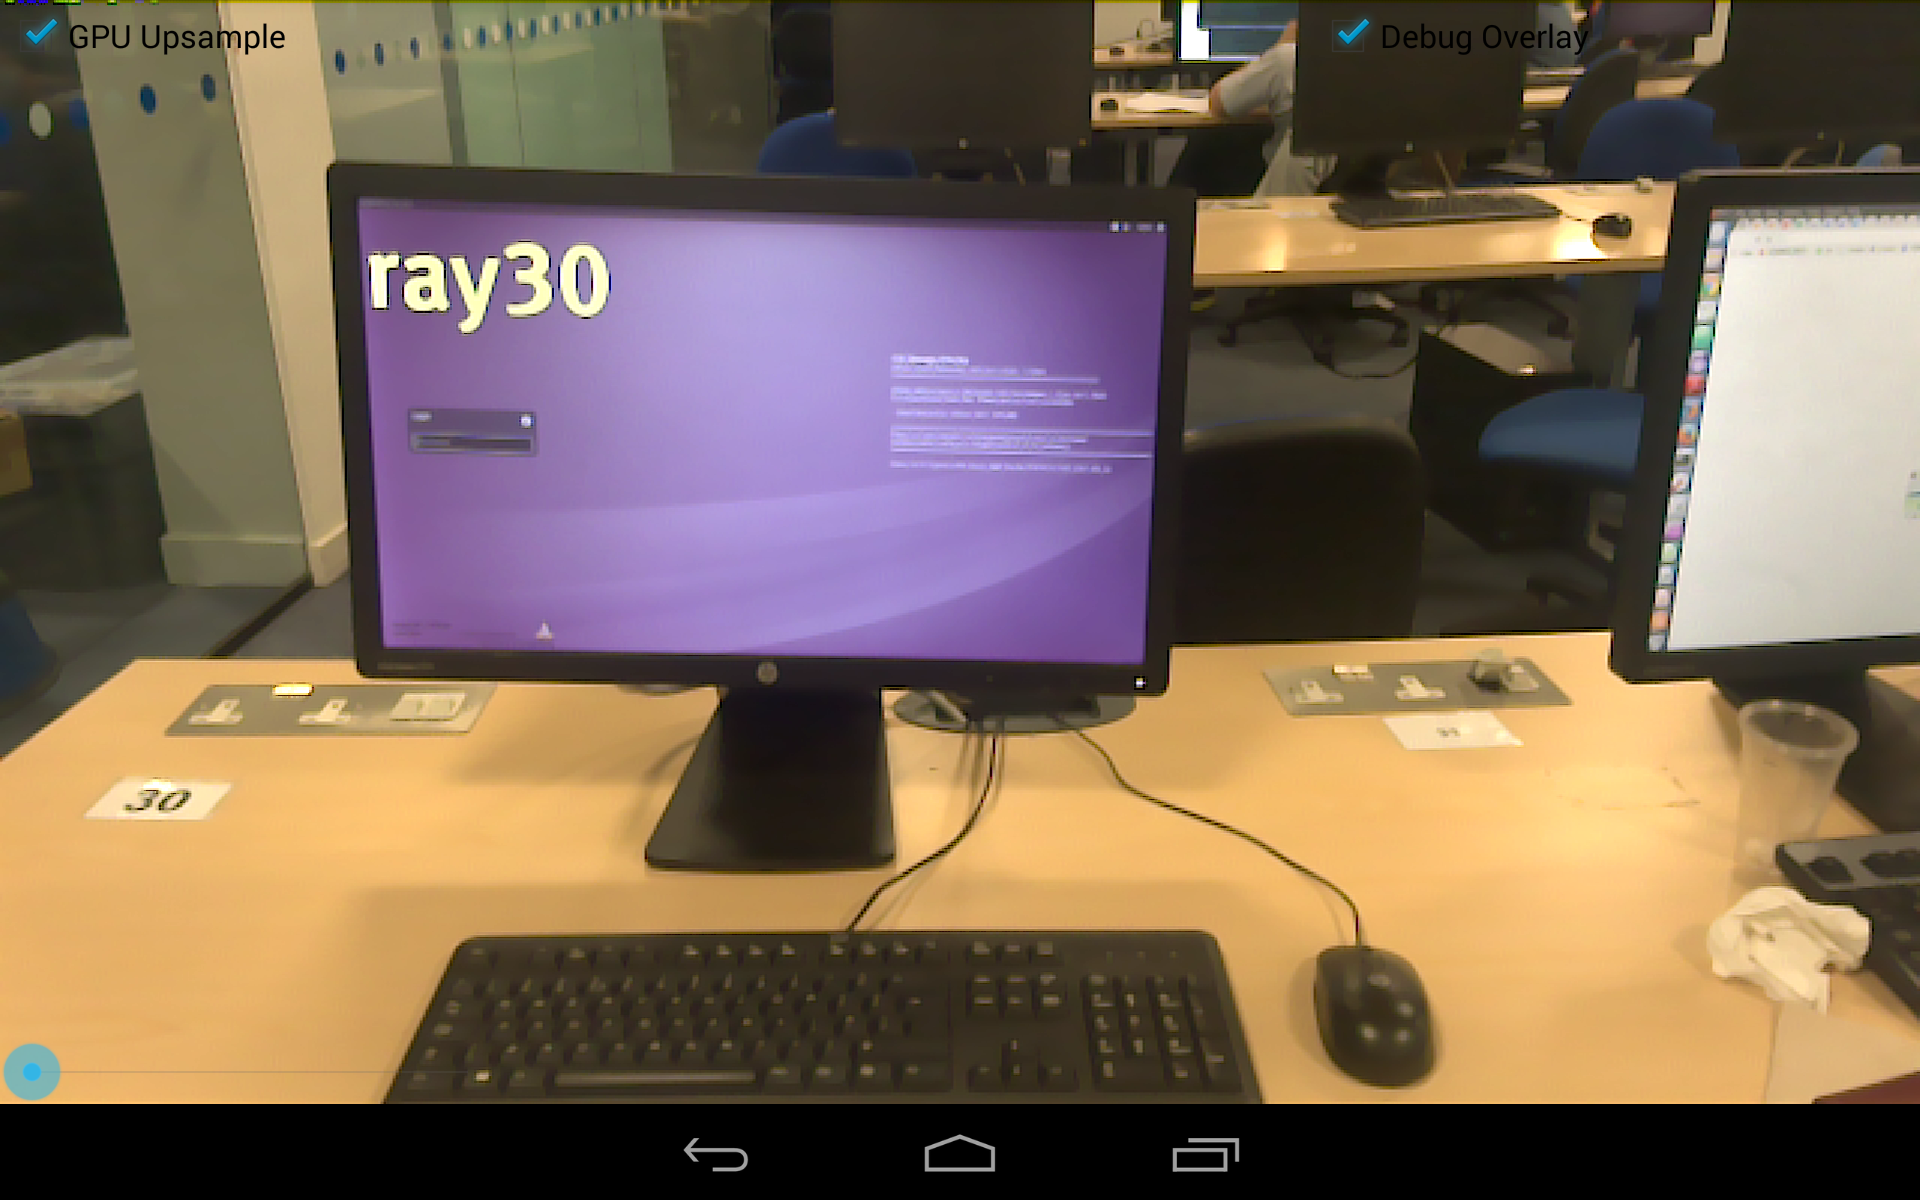
\includegraphics[width=0.7\textwidth]{figures/rgbd2}
    \caption{rgbd2}
    \label{fig: rgbd2}
\end{figure}

\begin{figure}[h]
    \centering
    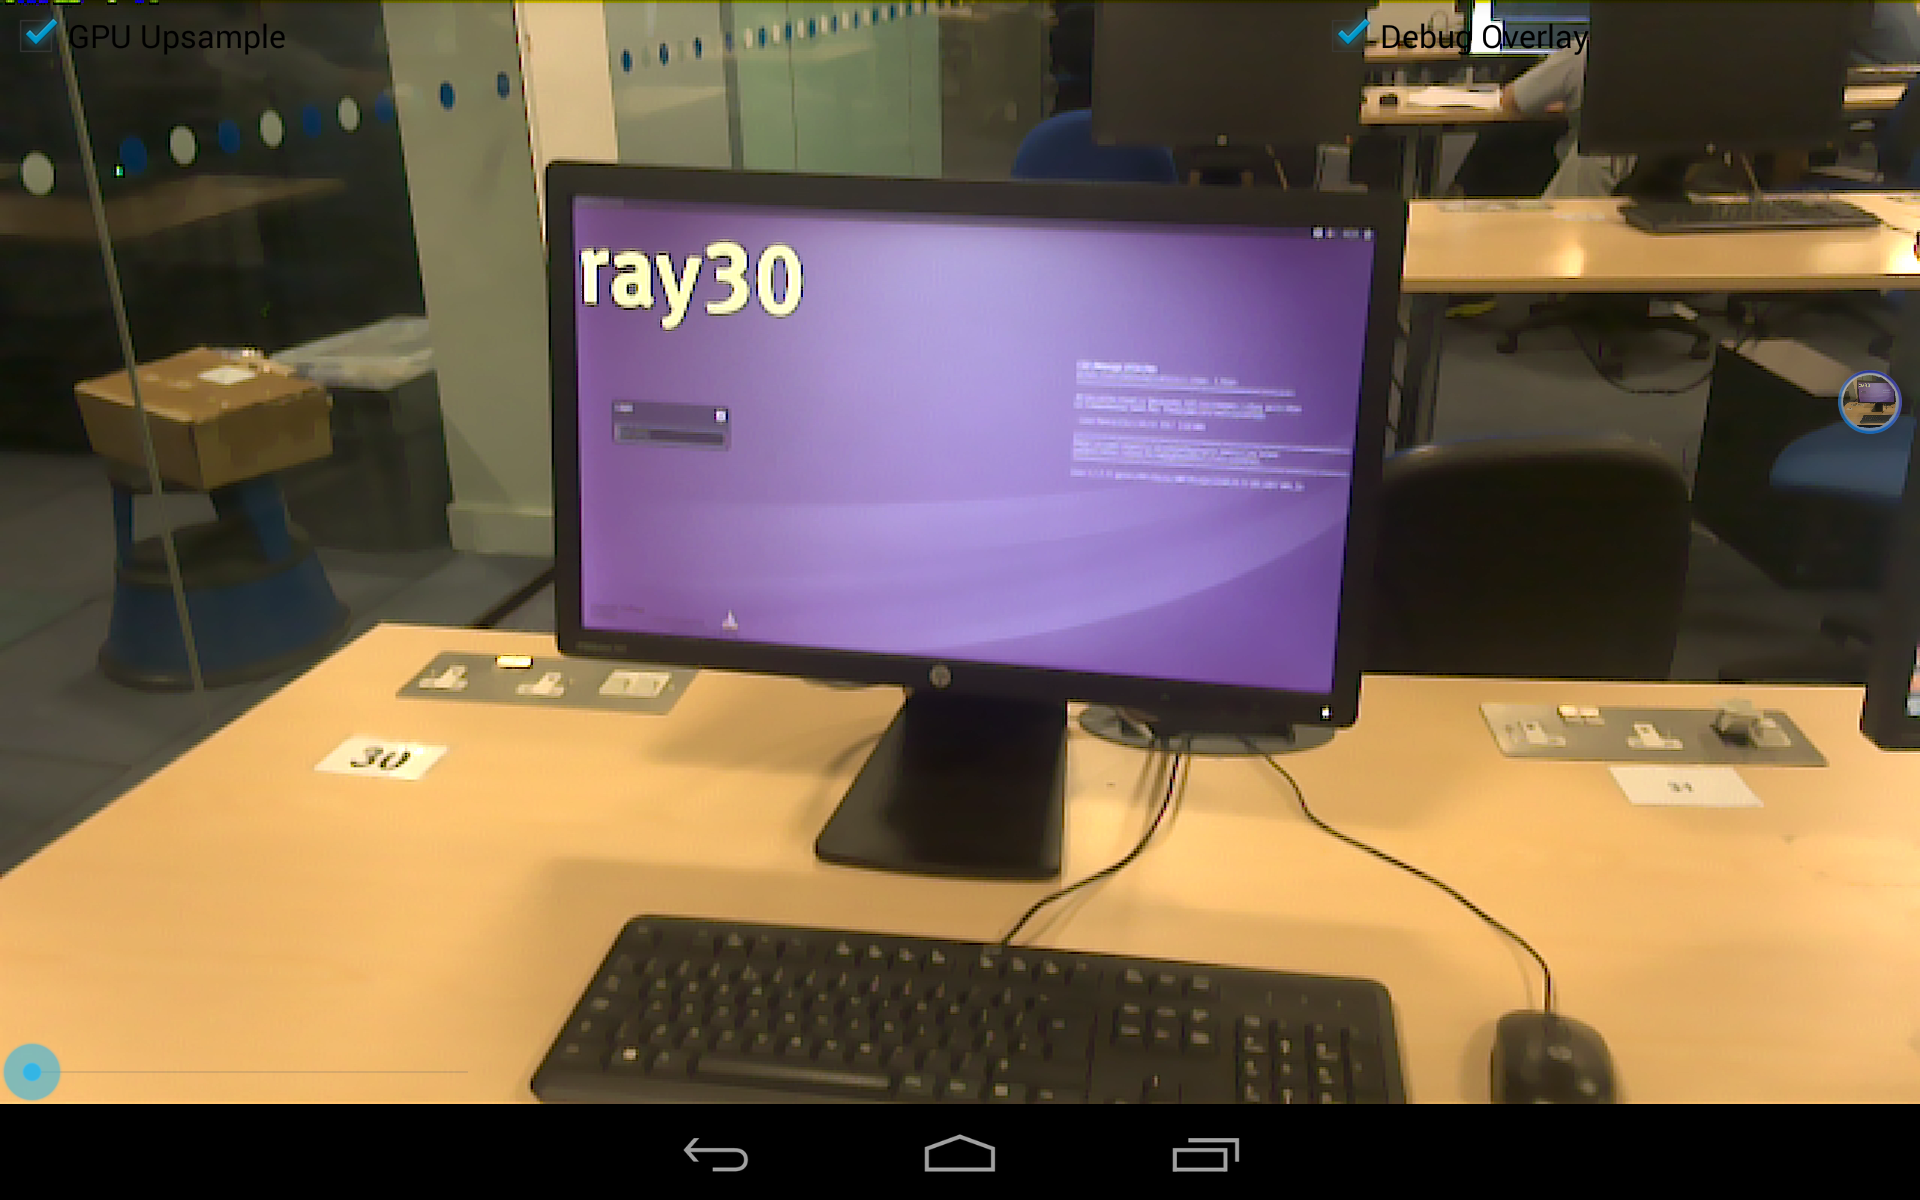
\includegraphics[width=0.7\textwidth]{figures/rgbd3}
    \caption{rgbd3}
    \label{fig: rgbd3}
\end{figure}

\begin{figure}[h]
    \centering
    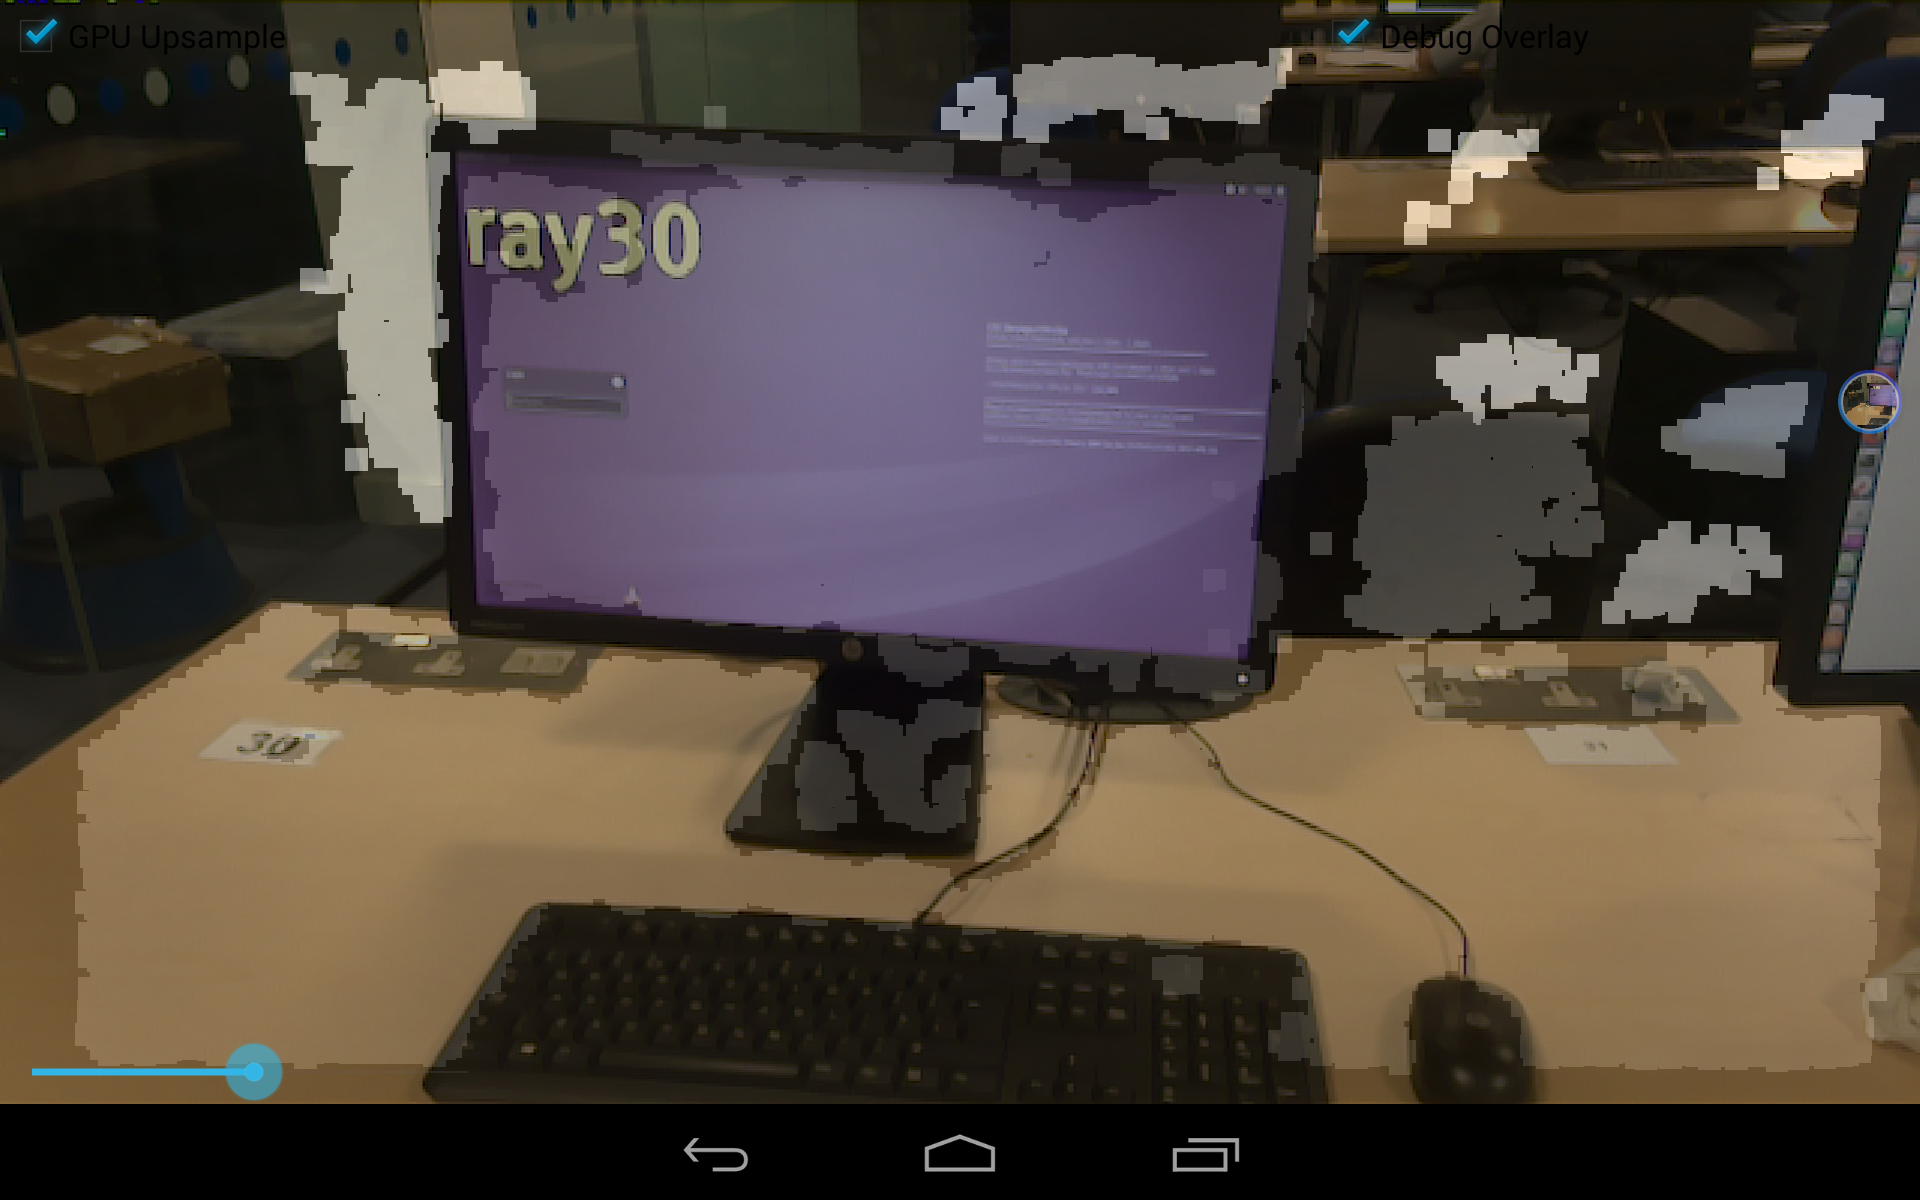
\includegraphics[width=0.7\textwidth]{figures/rgbd4}
    \caption{rgbd4}
    \label{fig: rgbd4}
\end{figure}

\begin{figure}[h]
    \centering
    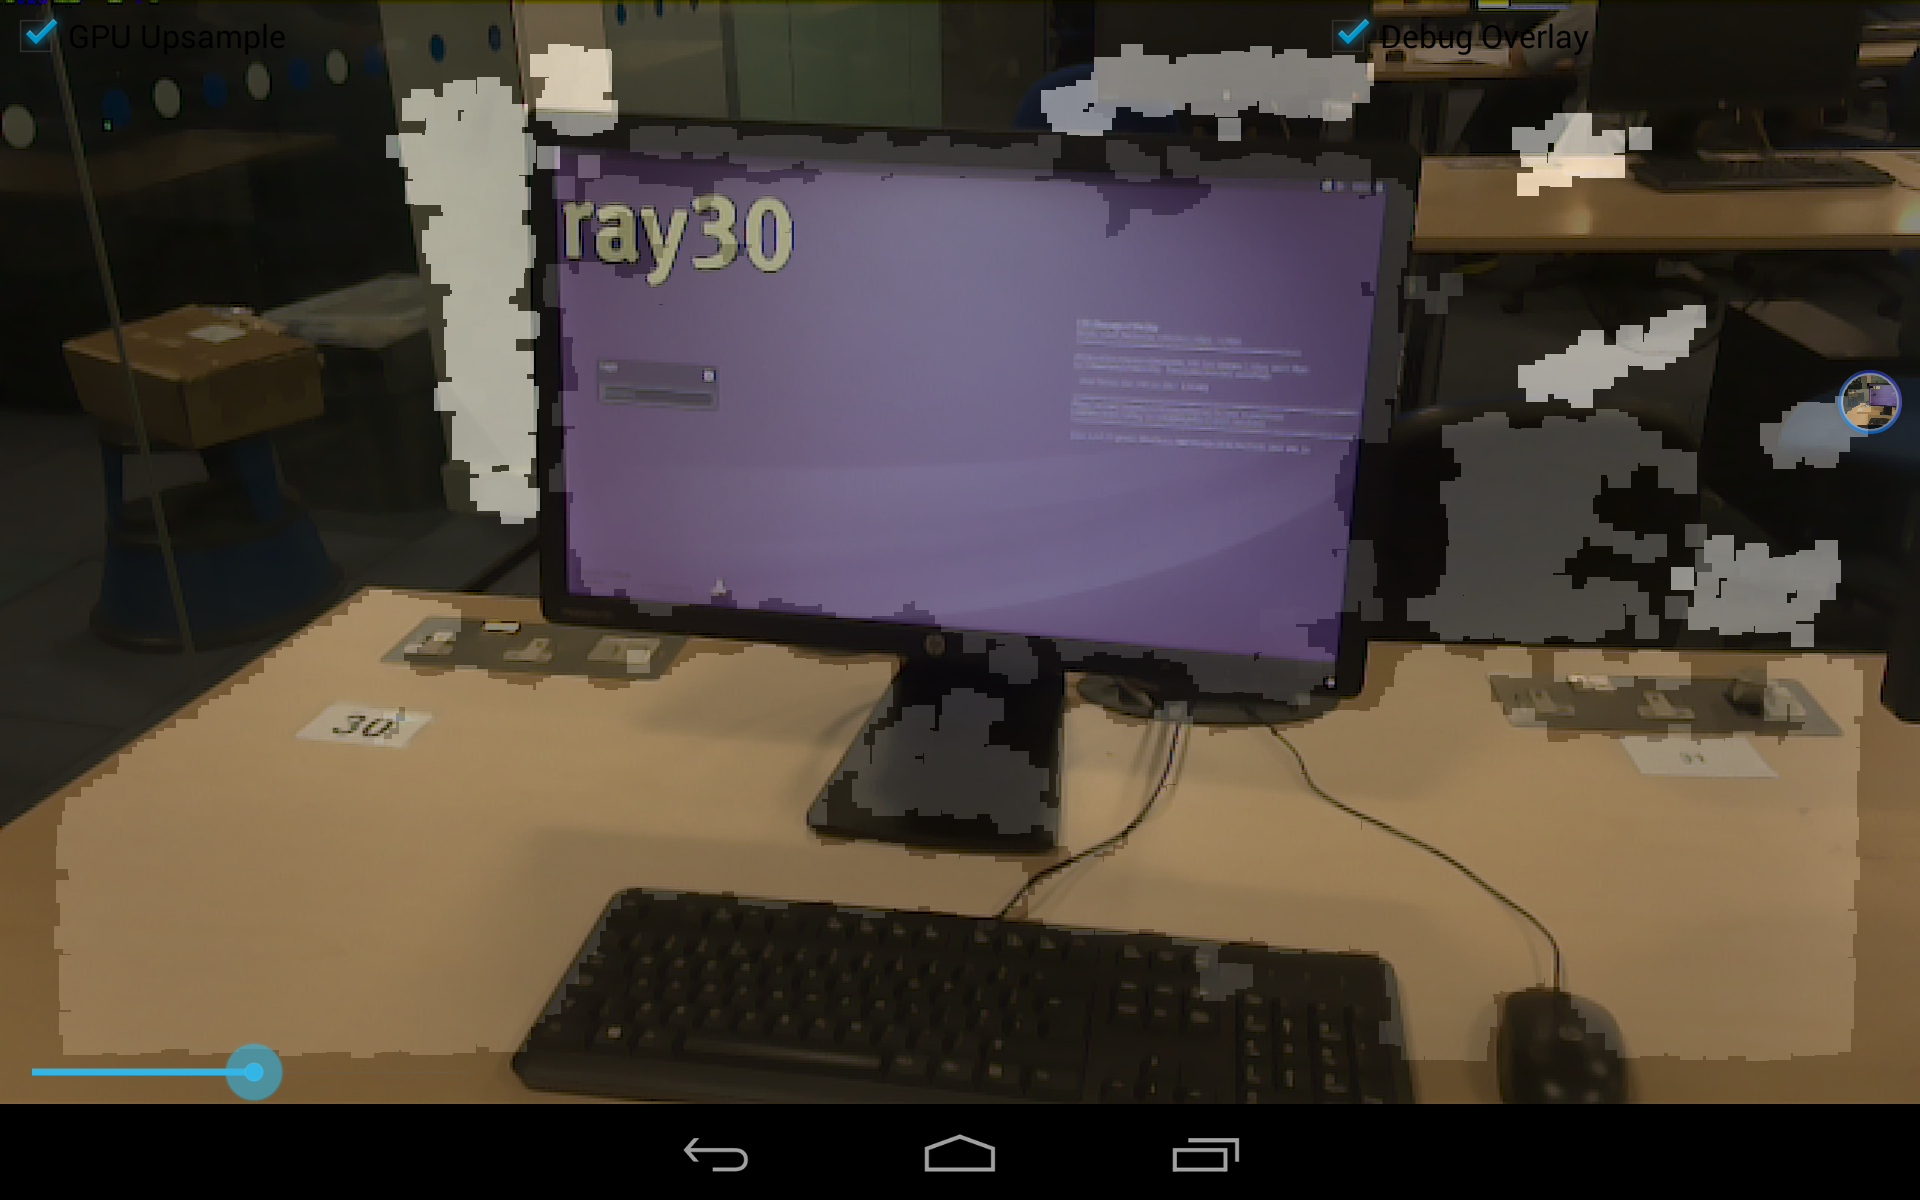
\includegraphics[width=0.7\textwidth]{figures/rgbd5}
    \caption{rgbd5}
    \label{fig: rgbd5}
\end{figure}

\begin{figure}[h]
    \centering
    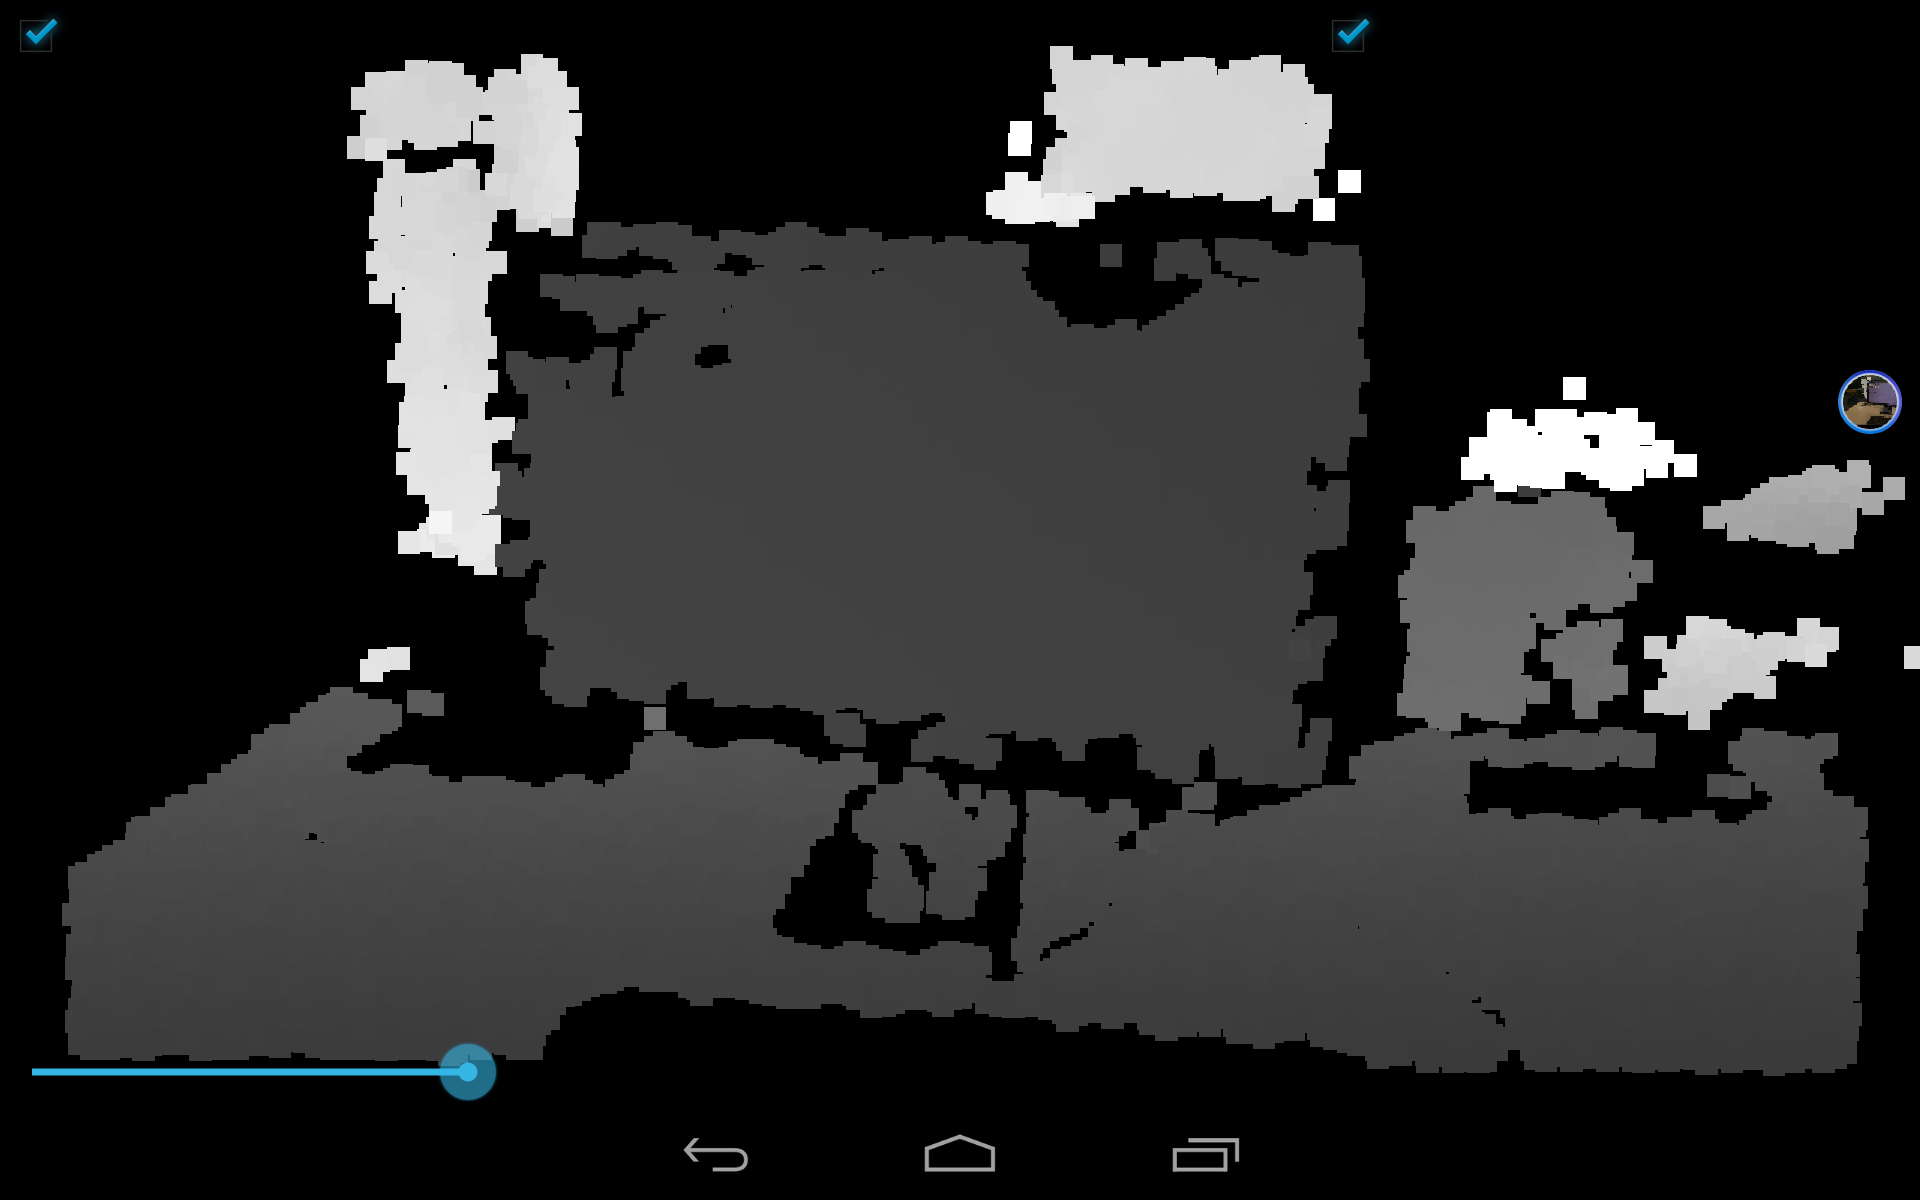
\includegraphics[width=0.7\textwidth]{figures/rgbd6}
    \caption{rgbd6}
    \label{fig: rgbd6}
\end{figure}


\newpage

\section{Project Implementation}

The central part of the report usually consists of three of four chapters detailing the technical work undertaken during the project. The structure of these chapters is highly project dependent. They can reflect the chronological development of the project, e.g. design, implementation, experimentation, optimisation, evaluation etc. although this is not always the best approach. However you choose to structure this part of the report, you should make it clear how you arrived at your chosen approach in preference to the other alternatives documented in the background. If you have built a new piece of software you should describe and justify the design of your program at some high level, possibly using an approved graphical formalism such as UML. It should also document any interesting problems with, or features of, your implementation. Integration and testing are also important to discuss in some cases. You need to discuss the content of these sections thoroughly with your supervisor.\\

============\\
\subsection{Environment Configuration}
In this project an Android application is developed to run on the Tango tablet. The Tango tablet runs Android 4.2.2 (KitKat), which corresponds to Android API 19. To be able to develop Android application, Eclipse Mars\footnote{\url{https://eclipse.org/mars/}} under Linux Ubuntu\footnote{\url{https://www.ubuntu.com/}} operating system is used with installed ADT(Android Development Tools)\footnote{\url{https://developer.android.com/studio/tools/sdk/eclipse-adt.html}} plugin. The reason for choosing Ubuntu environment is due to the NVIDIA Tegra Android Development Pack version \footnote{\url{https://developer.nvidia.com/AndroidWorks-TADP-Archive}} used for compiling CUDA part of ElasticFusion is only available on Ubuntu.\\
\\
After Eclipse and ADT plugin are installed, Android SDK for API version 19 and the corresponding Android NDK version r13b\footnote{\url{https://developer.android.com/ndk/downloads/revision_history.html}} is downloaded and their path is configured in Eclipse to allow Android NDK application to be developed for the Tango tablet.\\
\\
Lastly for using the Tango C API to develop Tango application on the tablet, the Tango Client API, Tango 3D Reconstruction API and the Tango Support API is needed, they can be downloaded from the Tango C API example repository on Github \footnote{\url{https://github.com/googlesamples/tango-examples-c}}. Also contained in the Tango C example repository the \textit{glm(OpenGL Mathematics)} library\footnote{\url{https://github.com/googlesamples/tango-examples-c/tree/master/third_party/glm}} that is used for matrix calculation is also imported along with the Tango C API files.



\subsection{Tango Platform}
Google's Tango\citep{tango} platform provides mobile devices with the abilities to sense the 3D space around the device and allow developers to build augmented reality applications on the device. Tango devices have three main functionalities: Motion Tracking, Area Learning, and Depth Perception, these are achieved using the RGB color camera, IMU (accelerometer and gyroscope), depth sensor and wide angle fisheye lens motion tracking camera on Tango devices. The motion tracking feature mainly estimate current position and pose of device using data from IMU and wide angle camera and techniques that use Kalman filter such as \citep{mourikis2007multi}. \\
\\
Given the cheap commodity mobile hardware and software, Tango device and tango platform provides the potential to build a fully self-contained 3D dense surface reconstruction solution using state-of-the-art RGB-D(color and depth) SLAM (Simultaneous Localization And Mapping) algorithms in this project. Among all the Tango devices that's released until the date when this report is written, there is the first Tango device the Tango “Peanut” mobile phone, the Tango "Yellostone" tablet, and Lenovo Phab 2 Pro mobile phone with the latest ASUS ZenFone AR phone. All of them are equipped with Android OS\footnote{\url{https://www.android.com/}}, but all the other devices carries Qualcomm processor, except for the "Yellostone" Tango tablet that's used in this project. The "Yellostone" Tango tablet carries Android 4.2.2 (KitKat) OS, this is the latest version of Android update it has until Google has officially stopped support for it. And it's equipped with a quadcore Nvidia Tegra K1 graphics card that supports CUDA(Compute Unified Device Architecture) function, which is used in the ElasticFusion program for camera tracking step. The Nvidia Tegra K1 processor has 192 CUDA cores, and supports CUDA 6.0 and OpenGL ES 3.1. The tablet also has 4GB of RAM shared by the CPU and GPU, an IMU that contains six-axis accelerometer and gyroscope, a wide FOV(field of view) motion tracking camera runs at 60Hz, and a projective depth sensor runs at 3Hz, and lastly a 4 MP RGB camera runs at 30Hz. The unique hardware configuration of the "Yellowstone" tablet mades it the perfect Tango device for this project, since with CUDA supported the ElasticFusion doesn't need a big rewrite for the camera tracking part.\\
\\
The Tango SDK for developers is offered in three programming languages: C and Java, Unity. The this project only the C API is used since C++ is what ElasticFusion is originally written, therefore using the Tango C API enables the code for Tango frontend to be combine with ElasticFusion without a huge amount of work for rewriting. Also the program runs faster in C under NDK environment on Android, where performance is crucial for the ElasticFusion program.\\
\\
The Motion Tracking feature on Tango platform provides the position and pose of Tango device of a certain frame with respect to a source frame at any time, the position and pose data is encapsulated inside a C++ struct \textit{PoseData}, the simplified version of this structure is given below.
\begin{lstlisting}
struct PoseData {
	double timestamp;
    double orientation[4];
    double translation[3];
}
\end{lstlisting}
The orientation array defines a quaternion that represents the rotation of the target frame with respect to the base frame. And the translation array represents the 3D vector of displacement between the target frame and the base frame. For the pose data to be able to be used by ElasticFusion, it have to be converted to affine transformation matrix, a transformation matrix is a 4 by 4 matrix with a 3 by 3 rotation matrix at left up corner and a 3D translation vector at the right most column. At time \textit{t} the global pose of the camera $\mat P_t$ (w.r.t. global frame $\xrightarrow{\textit{F}}_G$) can be shown below, where rotation matrix is $\mat R_t \in SO(3)$ and translation vector is $\vec t_t \in \mathbb{R}^3$.
\begin{align}
\mat P_t = \begin{bmatrix}
& R_t & t_t\\
0 & 0 & 0 & 1
\end{bmatrix} \quad  \in \mathbb{S}\E(3)
\end{align}
In the application, to get the pose of Tango device, the API function  is used, this function take a pair of frame reference, which represents the coordinate of frame that pose is in, in this case is \verb|TANGO_COORDINATE_FRAME_START_OF_SERVICE| and , means the pose would be the current device pose with respect to the pose device is in when application start. Another parameter is a callback function, the callback function will be called when a new Tango pose is available, and the pose data will be given in the parameter. The signature of this functions is given below.
\begin{lstlisting}
TangoErrorType TangoService_connectOnPoseAvailable(
    uint32_t count, const TangoCoordinateFramePair* frames,
    void (*TangoService_onPoseAvailable)(void* context,
                                         const TangoPoseData* pose)
\end{lstlisting}
Another way for getting pose data from Tango is the function \\
\verb|TangoService_getPoseAtTime|, this function pulls Tango pose data from the give as parameter, if this parameter is set to 0.0, the latest estimated pose is returned with respect to the coordinate of frames given. The signature of this function is shown below.\\
\begin{lstlisting}
TangoErrorType TangoService_getPoseAtTime(double timestamp,
                                          TangoCoordinateFramePair frame,
                                          TangoPoseData* pose);
\end{lstlisting}
The complete structure of Tango Pose Data struct is shown below, however only timestamp, orientation and translation are used to be processed for running ElasticFusion. \\
\begin{lstlisting}
typedef struct TangoPoseData {
  uint32_t version;
  double timestamp;
  double orientation[4];
  double translation[3];
  TangoPoseStatusType status_code;
  TangoCoordinateFramePair frame;
  uint32_t confidence;
  float accuracy;
} TangoPoseData;
\end{lstlisting}
In the Tango application developed, the RGB image data from color camera is not only being rendered to the screen, but also to be input to the ElasticFusion part for 3D reconstruction, and this is achieved by using Tango API and OpenGL ES textures. A class called \textit{GlCameraFrame} is responsible for manage OpenGL ES programs and shaders and texture, and then render the image stored in gl texture to the screen using function \textit{glDrawElements}. To acquire the RGB image from color camera and store it into textures, three Tango API functions are used. The first one is \verb|TangoService_connectTextureId| which the function signature is given below, it takes in a camera id, which in this case is \verb|TANGO_CAMERA_COLOR| for the color camera, and an OpenGL ES texture id. It connects the texture id of the texture to the camera which id is given in the parameter. This allows the second function \verb|TangoService_updateTexture| to be used, it updates the OpenGL ES texture that has been connected to the camera with id given in the parameter, fills in the latest image from that camera, and also returns the timestamps of the image acquired by the camera. The signature of this function is shown below. Lastly another function \verb|TangoService_updateTextureExternalOes| is used so that a specific OpenGL ES EXTERNAL OES texture can be filled with the image acquired by given camera id, it takes in valid OpenGL ES EXTERNAL OES texture id as parameter to update the texture associated with that id, the function signature is also given below.\\
\begin{lstlisting}
TangoErrorType TangoService_connectTextureId(
    TangoCameraId id, unsigned int tex, void* context,
    TangoService_OnTextureAvailable callback);
\end{lstlisting}
\begin{lstlisting}
TangoErrorType TangoService_updateTexture(TangoCameraId id, double* timestamp);
\end{lstlisting}
\begin{lstlisting}
TangoErrorType TangoService_updateTextureExternalOes(TangoCameraId id,
                                                     unsigned int tex,
                                                     double* timestamp);
\end{lstlisting}
After the RGB image data is stored in the OpenGL ES texture, these data can be read out from the OpenGL ES framebuffer that's associated with the texture using function \textit{glReadPixels}, the RGB data read out is store in a byte buffer which every value is corresponding to the RGB value of each pixel. This step is done in the \textit{GlCameraFrame} class, and the RGB data stored in byte buffer can be later used to write to files or feed into ElasticFusion program.\\
\\
Another function of Tango platform have been used in the application is Depth Perception, the depth data acquired from the depth sensor is stored in a C++ struct by tango call \textit{TangoPointCloud}, TangoPointCloud includes the time when the sensor captures this depth data, the number points contained in this data, and the array of 3D data points with their confidence level in the range of [0, 1]. In the 3D point coordinates, X and Y represents the position of data point corresponding to the pixel, and the Z component is the depth that was captured. The definition of this struct is shown below.\\
\begin{lstlisting}
typedef struct TangoPointCloud {
  uint32_t version;
  double timestamp;
  uint32_t num_points;
  float (*points)[4];
} TangoPointCloud;
\end{lstlisting}
On Tango platform, a struct called \verb|TangoSupportPointCloudManager| is used to manage point cloud data, it can move the pointcloud data from the callback thread to other threads for render or processing usage. The PointCloud manager is created using the function below where max\_points the maximum amount of 3D points allowed to be stored in it.\\
\begin{lstlisting}
TangoErrorType TangoSupport_createPointCloudManager(
  size_t max_points,
  TangoSupportPointCloudManager **manager
)
\end{lstlisting}
To register the call back for point cloud data, a similar function to pose data function is called, \verb|TangoService_connectOnPointCloudAvailable| takes in a call back function, so that it will be called when new pointcloud data is available. The function signature is given below.
\begin{lstlisting}
TangoErrorType TangoService_connectOnPointCloudAvailable(void(*)(void *context, const TangoPointCloud *cloud)
\end{lstlisting}
In the call back thread, point cloud manager is used to put the new point cloud data into the buffer within it, so that the data can be used later, the function\\
 \verb|TangoSupport_updatePointCloud| is called to swaps the buffer inside point cloud manager for new point cloud data.\\
\begin{lstlisting}
TangoErrorType TangoSupport_updatePointCloud(TangoSupportPointCloudManager *manager, const TangoPointCloud *point_cloud)
\end{lstlisting}
In other thread that does computation or rendering, point cloud data can be acquired from the point cloud manager use the function \\
\verb|TangoSupport_getLatestPointCloudAndNewDataFlag|, it returns the latest point cloud data stored inside the manager, and also returns a flag for the user to know whether the point cloud data acquired is new compared to the last time. The function signature is shown below.\\
\begin{lstlisting}
TangoErrorType TangoSupport_getLatestPointCloudAndNewDataFlag(
  TangoSupportPointCloudManager *manager,
  TangoPointCloud **latest_point_cloud,
  bool *new_data
)
\end{lstlisting}
After RGB and depth data is acquired, processing is needed to later usage, since both RGB and depth data are acquired with respect to their own sensors, therefore correction is needed to place the data under the same frame, in this application, the depth data is transformed to be align with the RGB data. However, the translation between depth sensor and color camera can not be simply calculated since the time of each data being captured is slight different. On tango platform, the function \verb|TangoSupport_calculateRelativePose| is used to calculate relative transformation between different coordinate of frame and timestamp, which in this case is \verb|TANGO_COORDINATE_FRAME_CAMERA_COLOR| and \\
\verb|TANGO_COORDINATE_FRAME_CAMERA_DEPTH|, this function outputs a Tango pose data instance to represent the related transformation calculated. This pose data is then converted into a transformation matrix to bring depth data into alignment with RGB data. The function signature is shown below.\\
\begin{lstlisting}
TangoErrorType TangoSupport_calculateRelativePose(double base_timestamp, TangoCoordinateFrameType base_frame, double target_timestamp, TangoCoordinateFrameType target_frame, TangoPoseData *base_frame_T_target_frame)
\end{lstlisting}
In the ElasticFusion program, the camera intrinsics data have to be provided for image processing, these information can be acquired directly on Tango using the Tango API, function \verb|TangoService_getCameraIntrinsics| returns a \verb|TangoCameraIntrinsics| struct instance corresponds to the input camera id. The Intrinsics struct contains the image width and height, focal length, and distortion coefficients. These information is later being input to the ElasticFusion. The function signature and struct definition is given below.\\
\begin{lstlisting}
TangoErrorType TangoService_getCameraIntrinsics(TangoCameraId cameraid, TangoCameraIntrinsics* intrinsics);
\end{lstlisting}
\begin{lstlisting}
typedef struct TangoCameraIntrinsics {
  TangoCameraId camera_id;
  TangoCalibrationType calibration_type;
  uint32_t width;
  uint32_t height;
  double fx;
  double fy;
  double cx;
  double cy;
  double distortion[5];
} TangoCameraIntrinsics;
\end{lstlisting}

\newpage

\subsection{Logging data from Tango}
After the RGBD and pose data from Tango are acquired, data of each frame is encapsulated into a C++ struct \textit{RGBDPosedata} and stored in a circular buffer. The definition of \textit{RGBDPosedata} is given below, other than RGBD and pose data, it also contains both the timestamp for depth and RGB data for calculating the transformation between color camera and depth sensor at the time their data is captured.\\
\begin{lstlisting}
struct RGBDPosedata {
  double pointCloudTimestamp;
  uint32_t pointCloudNumpoints;
  float *pointCloudPoints;
  uint8_t *image;
  double colorTimeStamp;
  int64_t m_lastTimestamp;
  TangoPoseData pose;
};
\end{lstlisting}
The first function implemented in the application developed is to write and RGBD and pose data recorded into their files, so that they can be used as dataset to run ElaticFusion on desktop computer. The processing of data into correct format is done in a data logging thread to reduce the workload on the main thread, and so that the writing of data is asynchronous with the capture for data. The circular buffer for storing data is an array of \textit{RGBDPosedata} structs with fixed size 50, after data is captured in the main thread and encapsulated into a \textit{RGBDPosedata} struct instance, it's stored in the position in circular buffer pointed by a variable called
\textit{latestBufferIndex}. This variable records the last position in the array where data is stored and so that data can be put into the front of array when the end of buffer is full, thus the circular effect is achieved where old data is gradually replaced by new data come in. This variable also allows the data logging thread to always read the latest frame of data that was stored in the buffer, in this way the speed difference between data producing and consuming is handled.\\
\\
The code processing and writing RGBD and pose data is combined and adapted from the Google Tango application RGB depth sync{\url{https://github.com/googlesamples/tango-examples-c/tree/master}} which produce a depth map in sync with the RGB image, and data logger for ElasticFusion\footnote{\url{https://github.com/mp3guy/Logger1}}, which originally is used to save data from RGBD camera that supports OpenNI\footnote{\url{https://structure.io/openni}} interface. Firstly the relative transformation between RGB and depth coordinate of frame and timestamp is calculated using the function \verb|TangoSupport_calculateRelativePose| which outputs a \textit{TangoPoseData} instance as result, this pose data is then converted into a transformation matrix for producing the depth map. To produce the depth map, firstly the 3D point coordinates in Tango point cloud is brought into alignment with RGB data using the transformation matrix calculated above, after that an upsample method is used filter the Tango Point Cloud data for smoothness, in the process the depth value of each 3D point coordinate in Tango Point Cloud is upsampled at a fixed size window around the 3D point's X and Y value, which corresponds to the pixel coordinates in the RGB image from color image. In this way, the depth map produced is in sync with the RGB image in both time and coordinate of frame, after that the data compressed for writing into files.\\
\\
In order to save space and reduce amount of data written to files, the RGB image data is compressed into JPEG format from byte buffer using the OpenCV library for Android\footnote{\url{http://opencv.org/platforms/android/}}, also the depth buffer is compressed using the \textit{compress2} function from zlib library\footnote{\url{http://zlib.net/}}. After that the timestamp, compressed RGB data and depth data with their sizes of each frame is written to the RGBD data file. and the pose data of each frame is written to the pose data file in the order of: \textit{x, y, z, qx, qy, qz, qw} where \textit{x, y, z} is the 3D position of the device and \textit{qx, qy, qz, qw} is the elements of quaternion that represents the orientation of the device.\\
\\
After the data being saved to two files on the Tango tablet, a slight modification is needed for the original ElasticFusion program to be able tu use them as datasets. The ElasticFusion program is designed to be able to use data from  datasets, however in the \textit{GIU} part of ElasticFusion program the \textit{Resolution} struct instance that holds width and height of RGB image is hard-coded with fix width and height, while the \textit{Intrinsics} struct instance can use the focal length and distortion parameter from a given calibration file, therefore a small change is made to the \textit{GIU} part of ElasticFusion program to allow for both image size and intrinsics data to be read from the calibration file.\\
\\
Using the logging function implemented in the application, experiments were carried out on desktop computer to run
ElasticFusion using data captured from the Tango tablet for 3D reconstruction, the screen shots of that is shown in Fig \ref{fig:Screenshot1}, Fig \ref{fig:Screenshot2}, Fig \ref{fig:Screenshot3} and Fig \ref{fig:Screenshot9}. From the screenshots it can be seen that the surface is able to be reconstructed however the points in the global map is vert sparse and the speed is very slow, this is mainly due to the noise and sparseness of depth data from depth sensor, also the pose estimated from Tango may not be very accurate, as the RGB image has even higher resolution (1980 x 720) then the image size in original ElasticFusion program. Also to allow for the surface to be reconstructed evenly instead of sparse points, when recording data using the Tango tablet, the device has to be held and move in a very slow and stable fashion. \\

\newpage

\subsection{Compiling ElasticFusion on Tango}
As mentioned above, the desktop ElasticFusion program includes three parts: the \textit{Core} part contains the code for ElasticFusion algorithm, and can be used as an API for other application, the \textit{GIU} part is responsible the displaying the user interface of program and handles input setting from the command line, reading from files provided for the program, the there is a \textit{GPUTest} program that user can test the performance of their GPU for running ElasticFusion. In this project the \textit{core} part is compiled and adapted on the Tango tablet to allow it to run on Android platform, and please be mindful that although open source code of ElasticFusion is available on Github\footnote{\url{https://github.com/mp3guy/ElasticFusion}}, in this project an internal version of source code is used for its better structure.\\

\subsubsection{Dependencies}
Originally in the ElasticFusion program, the dependencies include OpenGL 3.0\footnote{\url{https://www.opengl.org/}} that is used to manage the global map and predict the views, CUDA(Compute Unified Device Architecture) 7.0 that is used to implement the reduction process in camera tracking, OpenNI2\footnote{\url{https://structure.io/openni}} that is used to connect the program to a RGBD camera such as Microsoft Kinect or ASUS Xtion Pro Live. And SuiteSparse\footnote{\url{http://faculty.cse.tamu.edu/davis/suitesparse.html}} is used to do solve the Cholesky decomposition for optimization problem during camera tracking process. The header only library eigen3\footnote{\url{http://eigen.tuxfamily.org/index.php?title=3.0}} is used for matrix calculation. The zlib library\footnote{\url{http://zlib.net/}} is used uncompress depth data from dataset file and the libjpeg library\footnote{\url{http://libjpeg.sourceforge.net/}} is used to uncompress the RGB image data in dataset file from JPEG format into RGB pixel data. Lastly the Pangolin\footnote{\url{https://github.com/stevenlovegrove/Pangolin}} library that is used for building the GUI of program and also manage some OpenGL objects. Lastly the Boost C++ library\footnote{\url{http://www.boost.org/}} is mainly used for thread management in the application. \\
\\
Among the dependencies mentioned above, the OpenGL part in the source code of ElasticFusion is adapted to OpenGL ES for running on Android, and OpenNI is not used as since it's not needed in the Core part of ElasticFusion, the libjpeg library is removed and its function is implemented using OpenCV instead. Lastly the Pangolin library is removed and the part where it manages OpenGL objects is replaced with plain OpenGL ES implementation that is adapted from the Pangolin source code. The rest of dependencies are all compiled to be able to used in the Application for running on Android.\\

\subsubsection{Hardware requirements}
Since ElasticFusion is a RGBD SLAM system for 3D dense reconstruction, it needs to process full RGB image data as well as the depth map, also the pose estimation made heavily use of CUDA for GPU general data processing in the camera tracking stage if no dataset is provided, not to mention the local and global loop closure detection in each frame. Therefore by the hardware requirement for running ElasticFusion is already very high, quote from the \textit{README} of ElasticFusion on Github: "A very fast nVidia GPU (3.5TFLOPS+), and a fast CPU (something like an i7).", 3.5T FLOPS(Floating-point operations per second) is equal to 3500 G FLOPS, this kind of processing power is only available on graphics card like Nvidia GeForce GTX 970 which has 1664 CUDA cores. However the Nvidia Tegra K1 equipped on Tango tablet has only 192 CUDA core, and with 192 CUDA cores * 2 FLOPS per core * 950MHz, the processing power is only about 365 G FLOPS, which is approximately the power on a GT620 graphic card, only about one tenth what is required. This kind of processing power is considered quite high on a mobile device, however is still too low compare to the requirement.\\


\subsubsection{OpenCV}
The OpenCV library for Android\footnote{\url{http://opencv.org/platforms/android/}}\ is used to encode the RGB image data to jpeg when saving Tango data to files and used to decode the color image data from jpeg format to RGB pixel data when ElasticFusion is running using datasets on the Tango tablet.\\
\\
The Android version of OpenCV 2.4 source code in C++ is simply downloaded and imported in Eclipse as a project and attached to the Android application as a library. After that the android makefile of OpenCV \textit{OpenCV.mk} is included in the \textit{Android.mk} file of the Android application, so that OpenCV is compiled and linked as a static library for the application and the code in application can use it as normally done in C++ programs.\\

\subsubsection{CUDA}
CUDA (Compute Unified Device Architecture) is a compute platform for general purpose computing on Nvidia graphic card. CUDA 7.0 is needed in ElasticFusion program and since CUDA 6.0 supported by the NVIDIA Tegra K1 processer on Google Tango tablet, no change is needed to make to adapt this part of code. \\
In the \textit{core} part of the ElasticFusion code, a folder nameed \textit{CUDA} contains all the files that includes source code run on GPU using CUDA, include it there are normal C++ files and CUDA head files with extension ".cuh" and CUDA source files with extension ".cu".\\
\\
To compile the code inside this folder for the Android application on Tango tablet, under Ubuntu environment the NVIDIA Tegra Android Development Pack version 3.0r4\footnote{\url{https://developer.nvidia.com/AndroidWorks-TADP-Archive}} need to be download and installed. It contains the Android CUDA toolkit for CUDA 6.0 and can be used to compile CUDA code for Android platform.\\
\\
Firstly, the code in \textit{CUDA} folder is compiled into a static library by creating an \textit{"Android.mk"} makefile, in the makefile CUDA \textit{nvcc} compiler and \textit{g++} compiler from the Android standalone tool chain is used to compile the CUDA files and C++ files in the folder. After that a library file \textit{libCudaLib.a} is created and in the \textit{"Android.mk"} makefile for application the \textit{libCudaLib.a} is linked as a static library to the Android application. This allows the source code of ElasticFusion in C++ to call the CUDA code inside \textit{CUDA} folder and no change is needed to made.\\

\subsubsection{Pangolin}
The Pangolin\footnote{\url{https://github.com/stevenlovegrove/Pangolin}} library in the ElasticFusion source code was used to render the GUI of program and manage some OpenGL objects, however the \textit{Core} part of ElasticFusion does not contain GUI part and only use Pangolin in a few place, therefore compiling the Pangolin library on Android is an overkill. And so when porting the code for ElasticFusion onto Tango tablet, Pangolin is removed, and the part that Pangolin is used to manage encapsulated OpenGL objects is replaced by plain OpenGL ES code extracted from Pangolin's source code.\\
\\
The \textit{GlTexture} class in Pangolin stores an OpenGL texture object and its behaviour methods such as binding and uploading texture image. When adapting the ElasticFusion program on Tango tablet, the source code for \textit{GlTexture} class in Pangolin is extracted and put into a file in the ElasticFusion program, and then is place in ElasticFusion where Pangolin's \textit{GlTexture} is used is then replaced by the new \textit{GlTexture} class. The \textit{Shader} class originally in the ElasticFusion program is inherited from the \textit{GlSlProgram} class in Pangolin, it's mainly used for managing OpenGL programs and attached shaders. This class is adapted in a similar way, the part of source code that is useful in Pangolin is taken out and put inside the \textit{Shader} class. The \textit{GlRenderBuffer} and \textit{GlFramebuffer} class from Pangolin used are also adapted in similar way. The table \ref{table:Pangolin table} given below includes all the Pangolin values and class adapted or removed in the ElasticFusion program on Tango tablet.\\
\\
\begin{table}
\centering
\caption{Pangolin values and class adapted or removed}
\label{table:Pangolin table}
\begin{tabular}{|r|l|}
  \hline
  pangolin::GlTexture  \\
  pangolin::GlSlProgram  \\
  pangolin::GlSlVertexShader  \\
  pangolin::GlSlGeometryShader \\
  pangolin::GlSlFragmentShader  \\
  pangolin::GlRenderBuffer  \\
  pangolin::GlFramebuffer \\
   pangolin::OpenGlMatrix \\
    \hline
\end{tabular}
\end{table}


\subsubsection{SuiteSparse}
SuiteSparse\footnote{\url{http://faculty.cse.tamu.edu/davis/suitesparse.html}} is a suite of sparse matrix software, and it's used in the ElasticFusion program to do solve the Cholesky decomposition for optimization problem during camera tracking process. For doing Cholesky decomposition, the actual library used in ElasticFusion is the \textit{cholmod} library, however the \textit{cholmod} library depends on other libraries in SuiteSparse.\\
\\
The dependency of \textit{cholmod} library includes the \verb|SuiteSparse_config|, AMD, CAMD, CCOLAMD, COLAMD, CXSparse, clapack\footnote{\url{http://www.netlib.org/clapack/}} and metis\footnote{\url{http://glaros.dtc.umn.edu/gkhome/metis/metis/download}}. To compile \textit{cholmod} library for Android platform, first clapack and metis are compiled into static libraries since both their source code is not in the SuiteSparse source code. The srouce code for clapack is downloaded from the official website and the source code for metis-5.1.0\footnote{\url{https://github.com/scibuilder/metis}} is used. After they are compiled, two files \textit{libmetis.a} and \textit{libclapak.a} are generated, they are then used to compile the choldmod library using other compiled dependencies of cholmod library into a static library file. Finally the choldmod static library is linked in the \textit{Android.mk} makefile for Android application so that the cholmod library can be used.


\subsubsection{OpenGL}
OpenGL\footnote{\url{https://www.opengl.org/}} is used to manage map and predict views in the ElasticFusion program, it mainly made use of the transform feedback feature for off-screen rendering in OpenGL using the Vertex shader, Geometry shader and Fragment shader. To adapt this part of code on the Android platform for Tango tablet, the original OpenGL language need to be change to OpenGL ES language for mobile platform. The Tango tablet supports OpenGL ES version 3.1\footnote{\url{OpenGL ES 3.1 https://www.khronos.org/registry/OpenGL-Refpages/es3.1/}}, this is the latest version of OpenGL carried on Android API version 19, corresponds to Android 4.2.2 (KitKat), which is the last official update of Tango tablet gets. Since Google has officially stopped to support the Tango tablet, no newer version of Android can be installed and therefore newer version of OpenGL ES cannot be acquired on the tablet. The OpenGL ES version 3.1 on Tango tablet does not some features that's used in ElasticFusion program using OpenGL, so in some places workaround is used to adapt the code.\\
\\
Firstly, in the Android application on Tango tablet, OpenGL ES is already used to render the RGB image acquired from color camera to the screen, and the ElasticFusion program ported to the application is designed to be running on a separate thread. To let the ElasticFusion thread use OpenGL ES, a new OpenGL ES context need to be created and attached to the ElasticFusion thread, this is done by using the EGL\footnote{\url{https://www.khronos.org/egl}} platform available under Android NDK environment, a new EGL pixel buffer surface is created using the \textit{eglCreatePbufferSurface} function in EGL to allow for offscreen rendering into buffer using OpenGL ES in this thread. The EGL functions used to do that is given in the table \ref{table:EGL functions} below.\\
\\
\begin{table}
\centering
\caption{EGL functions used}
\label{table:EGL functions}
\begin{tabular}{|r|l|}
  \hline
  eglGetDisplay \\
 eglInitialize  \\
  eglChooseConfig  \\
  eglCreateContext \\
  eglCreatePbufferSurface  \\
  eglMakeCurrent  \\
    \hline
\end{tabular}
\end{table}
After the OpenGL ES context is created, original code in OpenGL needs to be adapted. In the original ElasticFusion code, the code for shaders are written in separate files and are read by Pangolin in the program to produce a C++ string of type \textit{const char *} that is then used as the source code for shaders by function \textit{glShaderSource}. However it will be troublesome to do the same thing on Android application, also because the Pangolin dependency is removed, the source code for shaders are all put into hardcoded C++ char array of type \textit{static const char []} for fast reading in a file, the source code string is then placed into a tupe together with the name of the shader for east identification of shader source code. The Geometry shader originally stored in the file \verb|copy_unstable.geom| is adapted and the created code is shown below as an example.\\
\begin{lstlisting}
static const char copy_unstablegeom_source[] =
    "#version 310 es\n"
    "#extension GL_EXT_geometry_shader : require\n"
    "precision highp float;\n"
    "precision highp int;\n"
    "layout(points) in;\n"
    "layout(points, max_vertices = 1) out;\n"
    "in vec4 vPosition[];\n"
    "in vec4 vColor[];\n"
    "in vec4 vNormRad[];\n"
    "flat in int test[];\n"
    "out vec4 vPosition0;\n"
    "out vec4 vColor0;\n"
    "out vec4 vNormRad0;\n"
    "void main() {\n"
    "    if(test[0] > 0) {\n"
    "        vPosition0 = vPosition[0];\n"
    "        vColor0 = vColor[0];\n"
    "        vNormRad0 = vNormRad[0];\n"
    "        EmitVertex();\n"
    "        EndPrimitive(); \n"
    "    }\n"
    "}\n";
static const std::tuple<std::string, std::string> copy_unstablegeom_tuple =
    std::make_tuple("copy_unstablegeom", copy_unstablegeom_source);
\end{lstlisting}
Other than putting the source code of shaders into char array, the actual code for shaders also need to be changed for OpenGL ES format, firstly the version indicator at the top of shader code is changed from \verb|#version 330 core| to \verb|#version 310 es| since the Tango tablet run at OpenGL ES version 3.1. Also the precision need to set for numerical types \textit{int} and \textit{float} and also the texture samplers. In OpenGL the data types  \textit{int} and \textit{float} can be converted to each other implicitly, however this has to be done explicitly in OpenGL ES so type conversion is manually added to the shader source code. Lastly in the code for Geometry shaders the OpenGL extension for it need to be declared using \\
\verb|#extension GL_EXT_geometry_shader : require|. The table \ref{table:OpenGL ES Shader} below gives all the declarations added to the beginning of shader source code.\\
\\
\begin{table}
\centering
\caption{OpenGL ES Shader adaptation}
\label{table:OpenGL ES Shader}
\begin{tabular}{|r|l|}
  \hline
  \verb| "#version 310 es\n" |\\
  \verb| "precision highp float;\n"| \\
  \verb|   "precision highp int;\n" |\\
   \verb|    "precision lowp sampler2D;\n"| \\
   \verb|  "precision lowp usampler2D;\n" |\\
 \verb|  "#extension GL_EXT_geometry_shader : require\n"| \\
    \hline
\end{tabular}
\end{table}
After the shader source code is adapted, other OpenGL code need to be changed as well. In OpenGL the format and internal format of textures can be totally different, for example in the ElasticFusion code RGB image texture format use \verb|GL_RGB| as format and \verb|GL_RGBA| as internal format, however this is not allowed in OpenGL ES, also some OpenGL texture formats used in the ElasticFusion program is not available in OpenGL ES, so adaptation is made using similar type of format such as changing from \verb|GL_RGB| to \verb|GL_RGBA| and use \verb|GL_RED| to replace \verb|GL_LUMINANCE|. Other than some function of transform back feature uses the Nvidia extension in OpenGL but not available in OpenGL ES, such as the \textit{glGetBufferSubData} function, this is replaced by the \textit{glMapBufferRange} function. With functions that simply doesn't exist in OpenGL ES and also no replacements like \textit{glDrawTransformFeedback}, a work around is used, by defining the function ourselves like below and using the \textit{eglGetProcAddress} function in EGL to retrieve the function pointer, the actual function pointer of OpenGL in driver of graphic card can be retrieved if they exist, then by casting the function pointer back to the function signature, this function can be used normally.\\
\begin{lstlisting}
void glDrawTransformFeedback(GLenum mode, GLuint id);
typedef void(GL_API_CALL_P PFNGLDRAWTRANSFORMFEEDBACKNVPROC)(GLenum mode, GLuint id);
\end{lstlisting}
The similar method is used to define the \verb|GL_GEOMETRY_SHADER| value for using Geometry shader, since the OpenGL ES version 3.1 on Tango tablet does not support Geometry shader on its own. However the OpenGL implementation inside the Nvidia Tegra K1 graphic card driver supports Geometry shader, so the work around is usable.\\
\\
Also in order to check for error in the OpenGL ES code, the function \textit{glGetError} and \textit{glCheckFramebufferStatus} are used to detect error and incorrect OpenGL ES framebuffer status that may not cause the application to crash, since normal OpenGL ES error will not be logged automatically. The function signatures are given below.\\
\begin{lstlisting}
GLenum glGetError(void);
GLenum glCheckFramebufferStatus(GLenum target);
\end{lstlisting}
A table \ref{table:OpenGL ES adaptation} is given below to list the adapted functions of OpenGL in the original ElasticFusio program.

\begin{table}
\centering
\caption{OpenGL ES adaptation}
\label{table:OpenGL ES adaptation}
\begin{tabular}{|r|l|}
  \hline
  original function or values & adaptation \\
  \hline
 glDrawTransformFeedback & extract function pointer using eglGetProcAddress\\
 \hline
 glGetBufferSubData  &  glMapBufferRange and glUnmapBuffer \\
 \hline
   \verb|GL_RGB|  & \verb|GL_RGBA| \\
   \hline
\verb|GL_LUMINANCE16UI_EXT| & \verb|GL_R16UI| \\
\hline
  \verb|GL_LUMINANCE_INTEGER_EXT| & \verb|GL_RED_INTEGER| \\
  \hline
\verb|GL_LUMINANCE32F_ARB| &  \verb|GL_R32F| \\
\hline
  \verb|GL_LUMINANCE| & \verb|GL_RED| \\
  \hline
  glGetVaryingLocationNV & removed \\
  \hline
  glTransformFeedbackVaryingsNV &\tabincell{c}{glTransformFeedbackVaryings, changed to be \\ used before linking the shader to OpenGL ES program} \\
  \hline
 glPushAttrib & removed \\
 \hline
 glPopAttrib & removed\\
    \hline
\end{tabular}
\end{table}





\subsubsection{Eigen}
Eigen\footnote{\url{http://eigen.tuxfamily.org/}} is a C++ template library for linear algebra: matrices, vectors, numerical solvers, and related algorithms. In the ElasticFusion program, Eigen is used to store the position and pose data uisng Eigen structures like \textit{Eigen::Vector4f} for homogeneous coordinates and \textit{Eigen::Matrix4f} or \textit{Eigen::Isometry3f} for pose data representing in affine transformation matrix.\\
\\
Eigen3\footnote{\url{http://eigen.tuxfamily.org/index.php?title=3.0}} source code is used in the Application on Tango tablet, since it's just a header only library that uses templates, the source code folder is pasted in the project source code and the header needed is simply included in the code that use Eigen.\\



\subsubsection{Eigen}
In the Android application developed on Tango tablet, Boost\footnote{\url{http://www.boost.org/}} is mainly use for manage thread, such as creating new thread to compress RGB image and depth data in the data logging function, or creating new thread to run ElasticFusion program. The version of Boost used in the application is 1.53.0\footnote{\url{http://www.boost.org/doc/libs/1_53_0/}}, the source code is downloaded from Github\footnote{\url{https://github.com/emileb/Boost-for-Android-Prebuilt}}, which is a built version of Boost for Android using the code from \url{https://github.com/sorccu/Boost-for-Android}. The Boost library is compiled into a static library and it's linked to the main application in the \textit{Android.mk} makefile.


\newpage



\subsection{Running ElasticFusion on Tango}

After the ElasticFusion program is compiled on the Tango tablet, actual functions need to be implemented to run the ElasticFusion program using different data sources. In the Android application developed in this project, the ElasticFusion can be either run using the live RGBD and pose data from the cameras and IMU sensor on board, or run using the \verb|dyson_lab.klg| dataset that was used as the example in ElasticFusion paper\citep{whelan2016elasticfusion}, or running using the Tango RGBD and pose data saved earlier in files. However, they are all implemented in similar way by starting a new thread to run ElasticFusion. \\

\subsubsection{Running ElasticFusion using data from Tango}
To run the ElasticFusion program using the RGBD and pose data from Tango tablet, a similar method like the data logging function is used. When the button for this function is pressed on screen, the function called is passed from the event listener in Java part of the application to the C++ part using the Java Native Interface (JNI) on Android platform. Firstly it is checked that no other function is running before the ElasticFusion thread can start, after that when the function started, the RGBD and pose data from Tango will be put into the circular buffer of \textit{RGBDPosedata} structures in the class for this function.\\
On the other hand, a new ElasticFusion running thread starts when the button is pressed, firstly a new OpenGL context is created and attached to the current thread as described above, and then the \textit{Resolution} and \textit{Intrinsics} structs from ElasticFusion are configured using Tango camera data acquired use the \\
\verb|TangoService_getCameraIntrinsics| function. After that the \textit{ElasticFusion} class is initialised using configurations that makes the program run at fastest speed, such as disable SO(3) pre-alignment, enabling fast odometry by using single level tracking pyramid, disable pose bootstrap, and disable loop closure detection function. Also the \textit{confidenceThreshold} value is set to 0.45 instead of the default value 10.0, the reason for doing it will be explain later. Before the ElasticFusion can process any data, OpenGL ES is configured using the code shown below in Table \ref{table:OpenGL ES configuration}.\\
\begin{table}
\centering
\caption{OpenGL ES configuration}
\label{table:OpenGL ES configuration}
\begin{tabular}{|r|l|}
  \hline
 glReadPixels \\
   \hline
 \verb|glPixelStorei(GL_UNPACK_ALIGNMENT, 1);|\\
   \hline
 \verb|glPixelStorei(GL_PACK_ALIGNMENT, 1);|\\
   \hline
  \verb|glEnable(GL_DEPTH_TEST);|\\
    \hline
  \verb|glDepthMask(GL_TRUE);|\\
    \hline
  \verb|glDepthFunc(GL_LESS);|\\
    \hline
\end{tabular}
\end{table}
After the set up is done, inside a whileloop the latest RGBD and pose data structure instance from the circular buffer is read out if new data is available. Then the RGBD and pose data is converted into the correct format for ElasticFusion to process.\\
\\
In the adaptation of OpenGL code to OpenGL ES code, the format of RGB image has to be changed from \verb|GL_RGB| to \verb|GL_RGBA| in order to match the limitation of OpenGL ES, therefore in order to use the color image data in \verb|GL_RGBA| format when the image data is read out in the \textit{GlCameraFrame} class using the \textit{glReadPixels} function, it's read out in \verb|GL_RGBA| format instead of the \verb|GL_RGB| format used in data logging function.\\
\\
In the data processing stage, the depth data is brought into alignment with the camera data coordinate of frame,  upsampled use the same method as in data logging function and converted to millimetre scale to produce a depth map, and the pose data is converted into a \textit{Eigen::Matrix4f} structure for ElasticFusion.\\
\\
Then the data is processed by calling the \textit{processFrame} function of ElasticFusion with RGB image data, depth data, pose and timestamp, which the function signature is shown below.
\\
\begin{lstlisting}
void processFrame(const unsigned char *rgb, const unsigned short *depth,
const int64_t &timestamp, const Eigen::Matrix4f *inPose = 0,
const float weightMultiplier = 1.f,
const bool bootstrap = false);
\end{lstlisting}
After a frame is processed, the state of ElasticFusion program can be checked by getting some critical values store in it such as the current number of surfels in the global map or the number of frames storing in the fern database. These data is logged out and can be viewed using the \textit{adb logcat} command on computer if the Tango tablet is
connecting to it.\\
\\
The purpose of running ElasticFusion program is to dense 3D reconstruction of the space that the Tango tablet is scanning, therefore the 3D reconstructed map by ElasticFusion must be able to saved in a ply file for viewing or other usage as the desktop version does. On the application developed this can be done by simply pressing the "save" button on screen, this will set a thread safe flag using mutex lock, so that after a data frame is processing when the ElasticFusion thread checks this flag, it will save the map if the flag is set. The saving of is map into ply file is the same as in original ElasticFusion program, the map is downloaded as 3D points from the \textit{Globalmodel} class and then each point's confidence value is checked against the \textit{confidenceThreshold} value set before, if the point's confidence value is above the threshold then it's saved to the file. The saved ply file is supposed to be able to view on applications on the Tango tablet such as "MeshLab for Android", however no attempt is successful for unknown reason.\\
\\
In order to show the speed of ElasticFusion running, a frame counter is displayed on the screen in application, every time the ELasticFusion processed a frame, the frame counter is incremented. This is done by when the screen is rendered by using the \verb|request_render}| function, the increment function is called from the C++ part to the Java part of program using Java Native Interface (JNI), this function call in Java then starts a new \textit{Runnable} using the\textit{runOnUiThread} function to increment the counter and set the text of the counter label.\\

\subsubsection{Running ElasticFusion dataset on Tango}









\subsubsection{Running Tango dataset on Tango}












\newpage



\subsection{Combine ElasticFusion with pose from Tango in Loop closure mode}





\subsection{Debugging and testing}



\newpage






\begin{figure}[h]
    \centering
    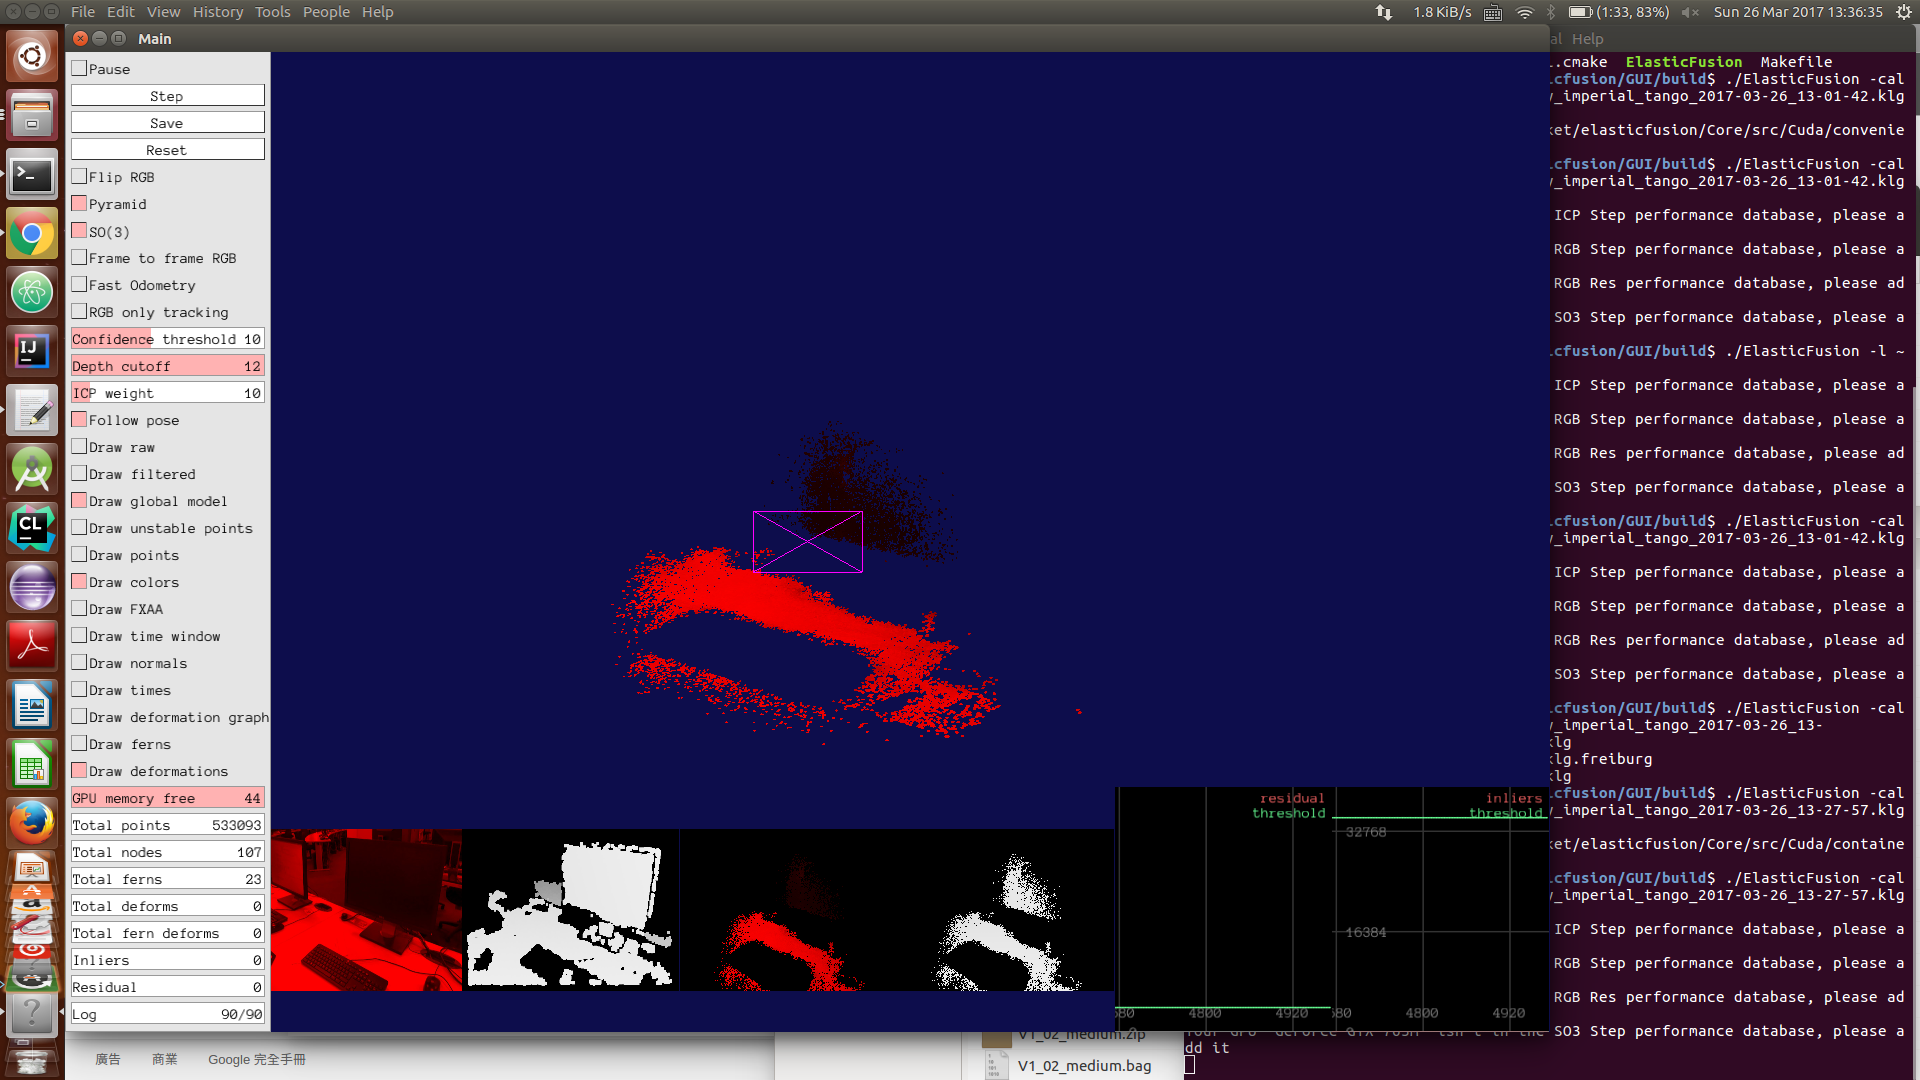
\includegraphics[width=0.7\textwidth]{figures/Screenshot1}
    \caption{Screenshot1}
    \label{fig:Screenshot1}
\end{figure}

\begin{figure}[h]
    \centering
    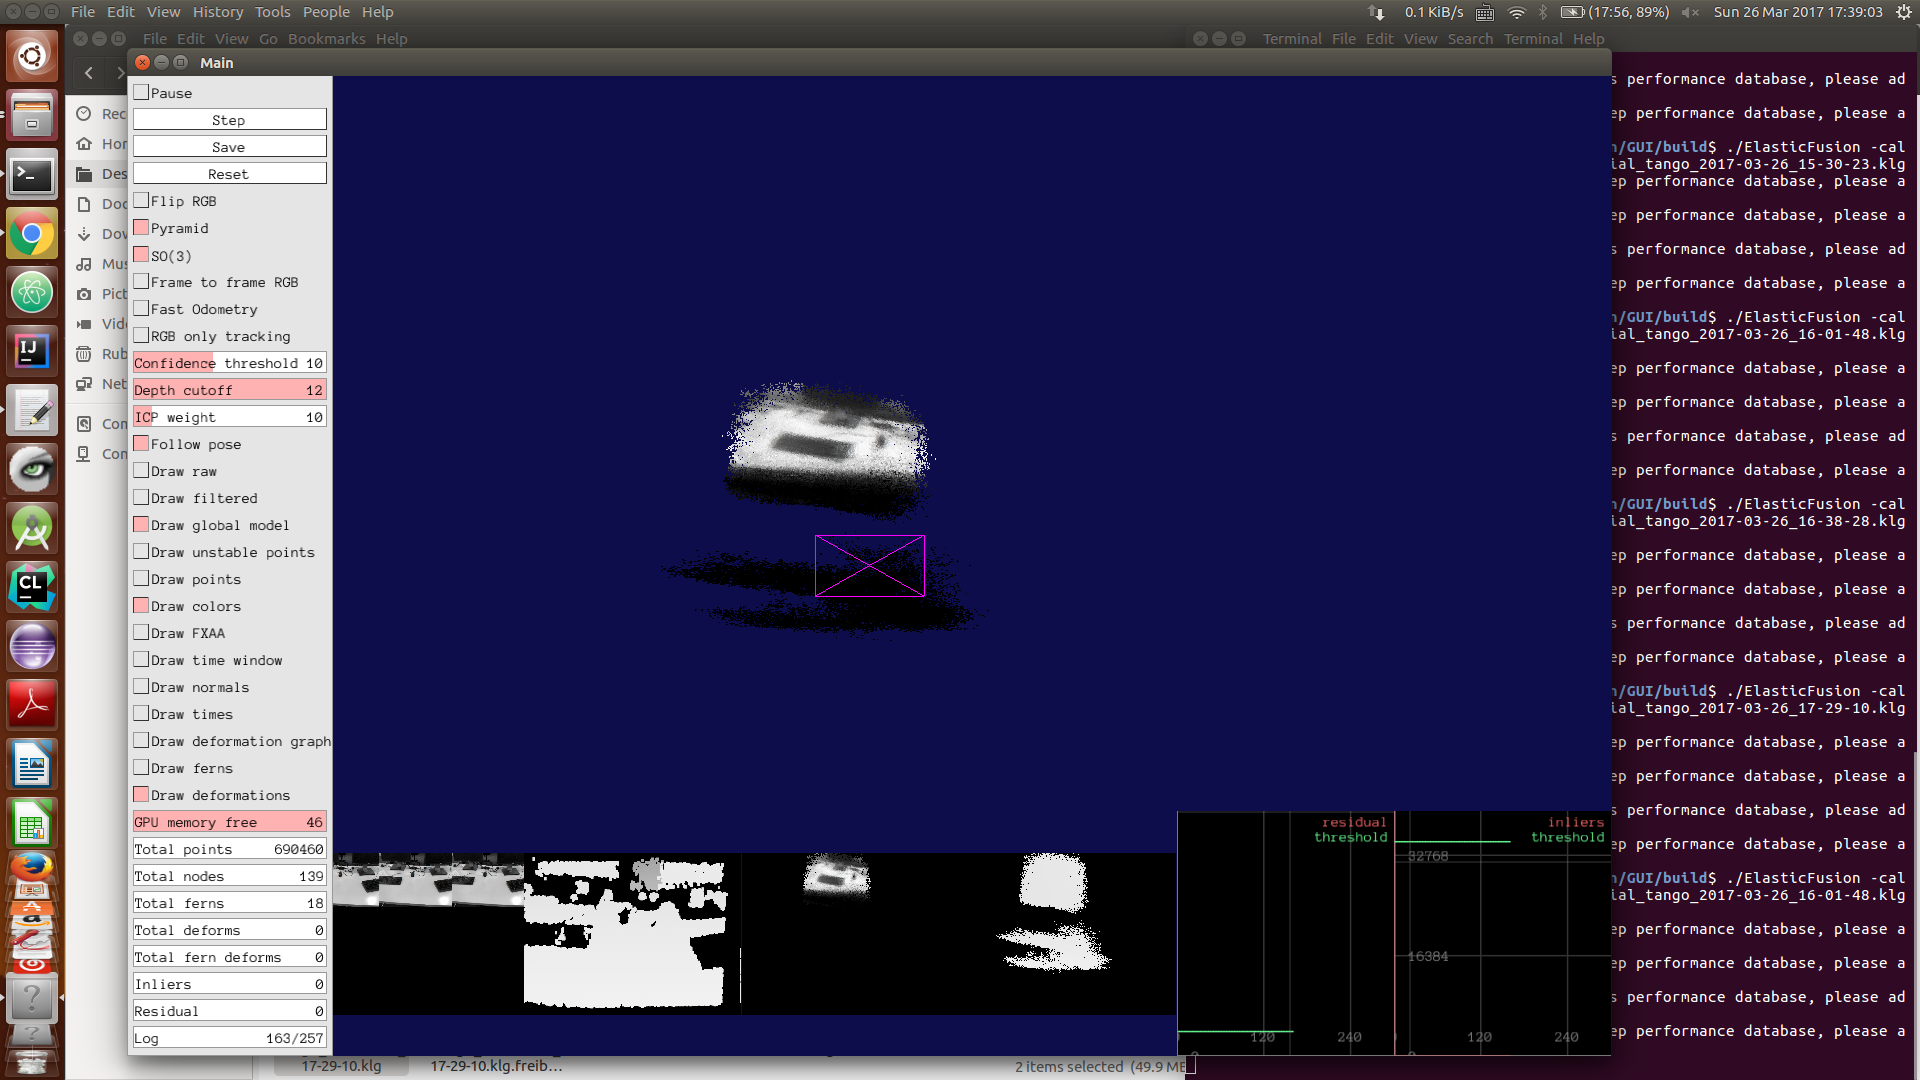
\includegraphics[width=0.7\textwidth]{figures/Screenshot2}
    \caption{Screenshot2}
    \label{fig:Screenshot2}
\end{figure}

\begin{figure}[h]
    \centering
    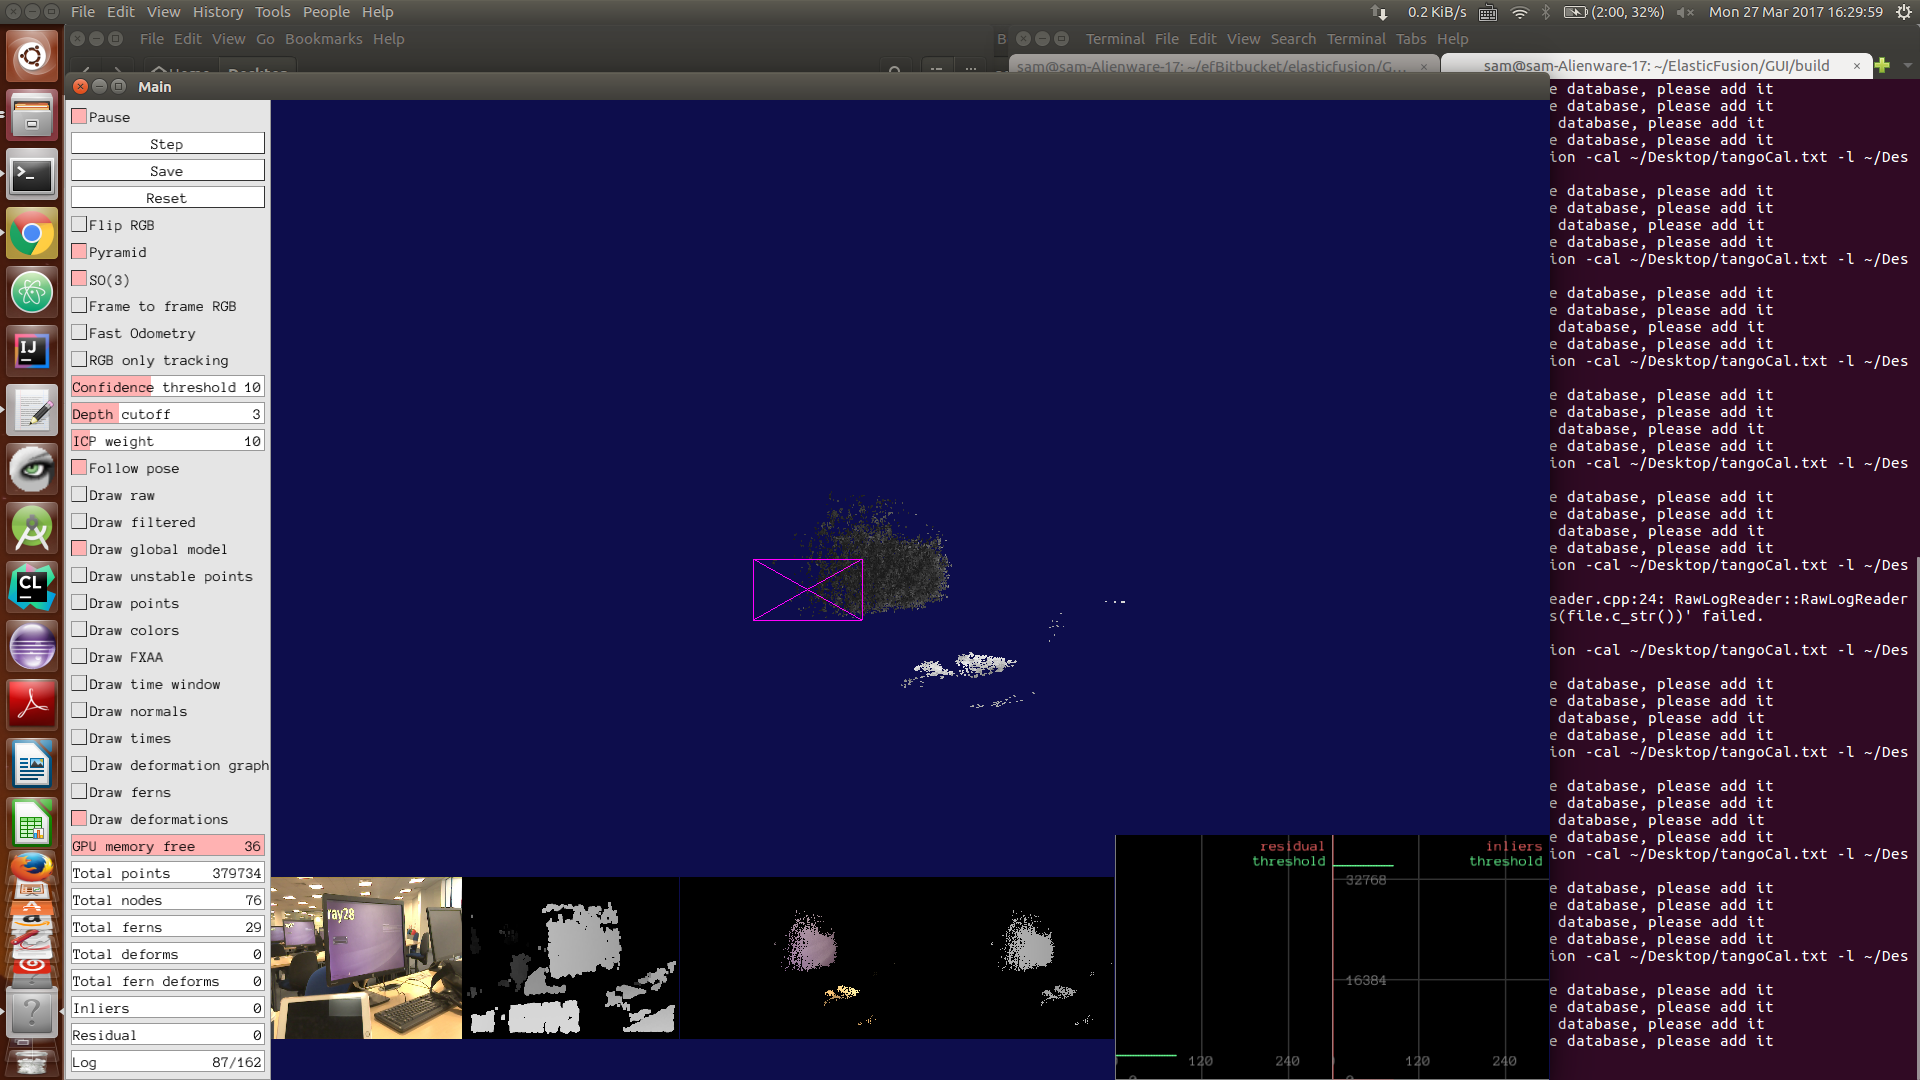
\includegraphics[width=0.7\textwidth]{figures/Screenshot3}
    \caption{Screenshot3}
    \label{fig:Screenshot3}
\end{figure}

\begin{figure}[h]
    \centering
    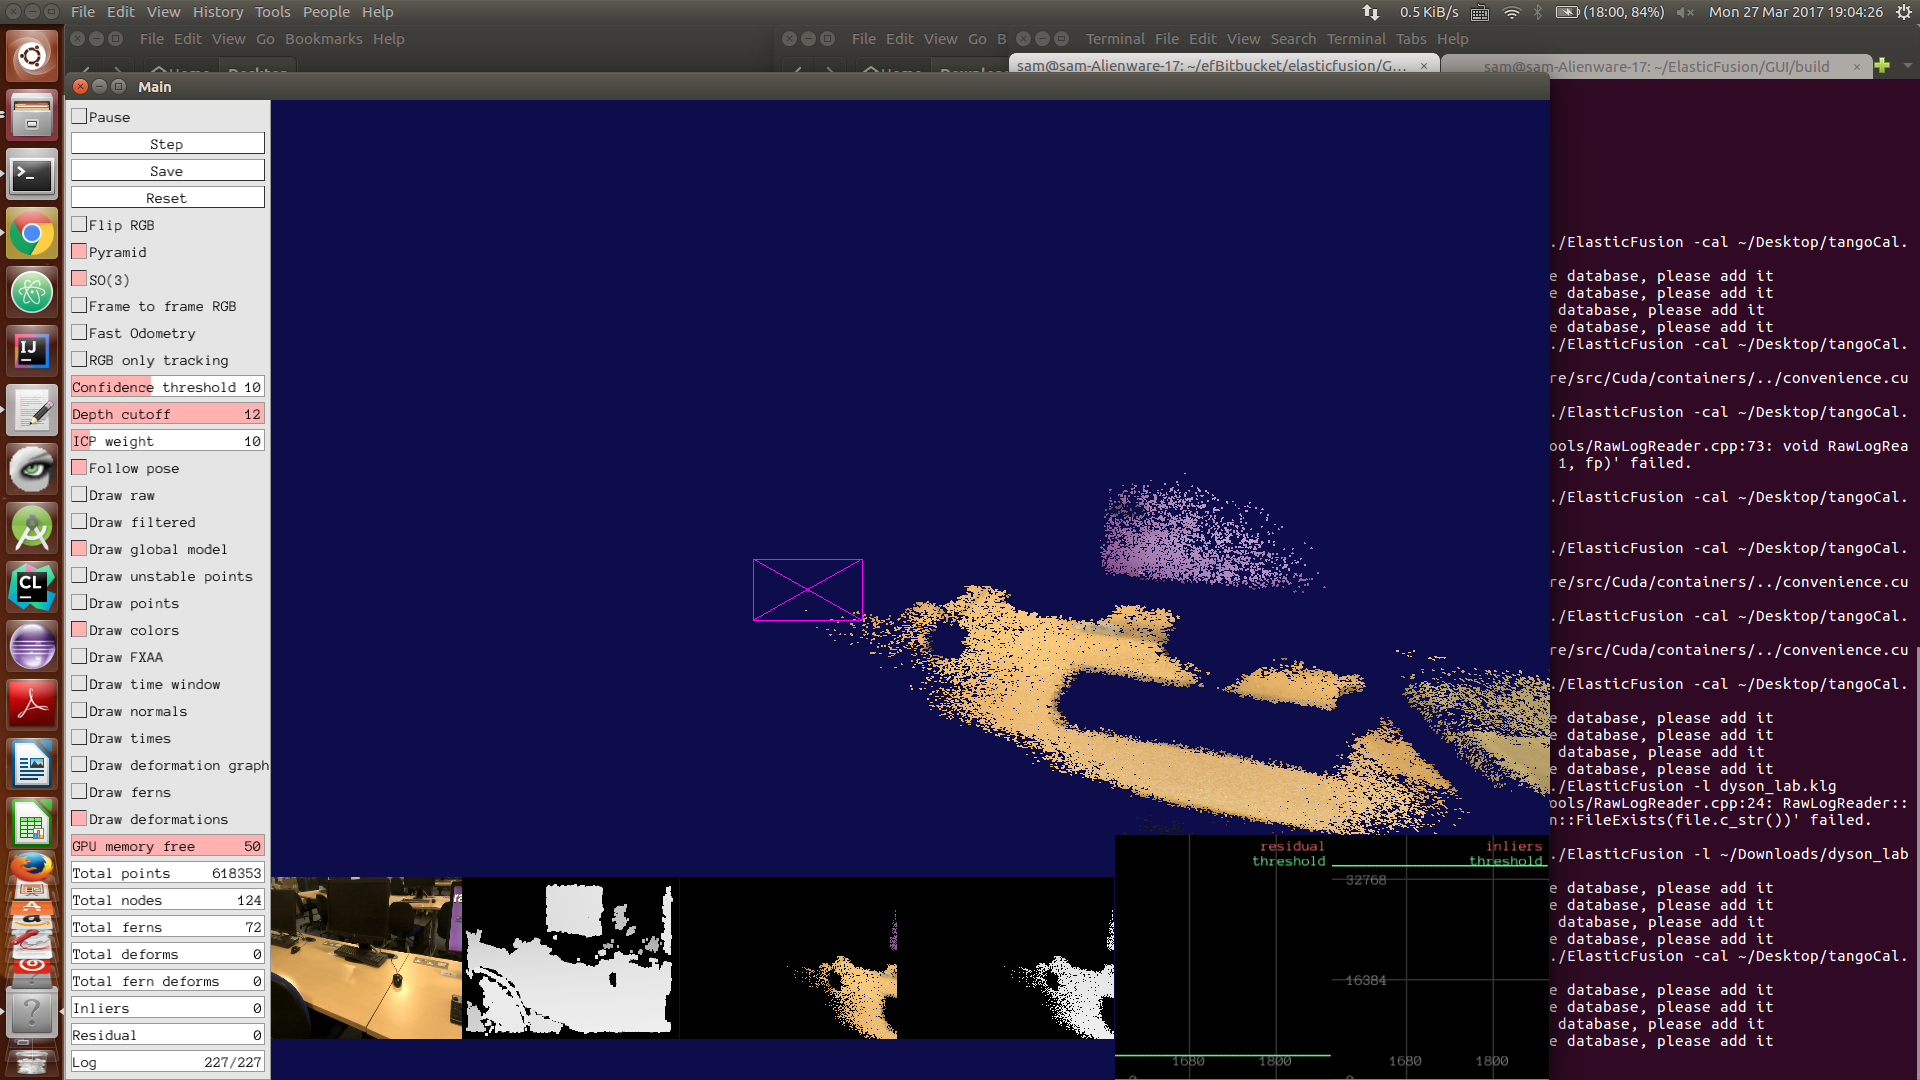
\includegraphics[width=0.7\textwidth]{figures/Screenshot9}
    \caption{Screenshot9}
    \label{fig:Screenshot9}
\end{figure}


\begin{figure}[h]
    \centering
    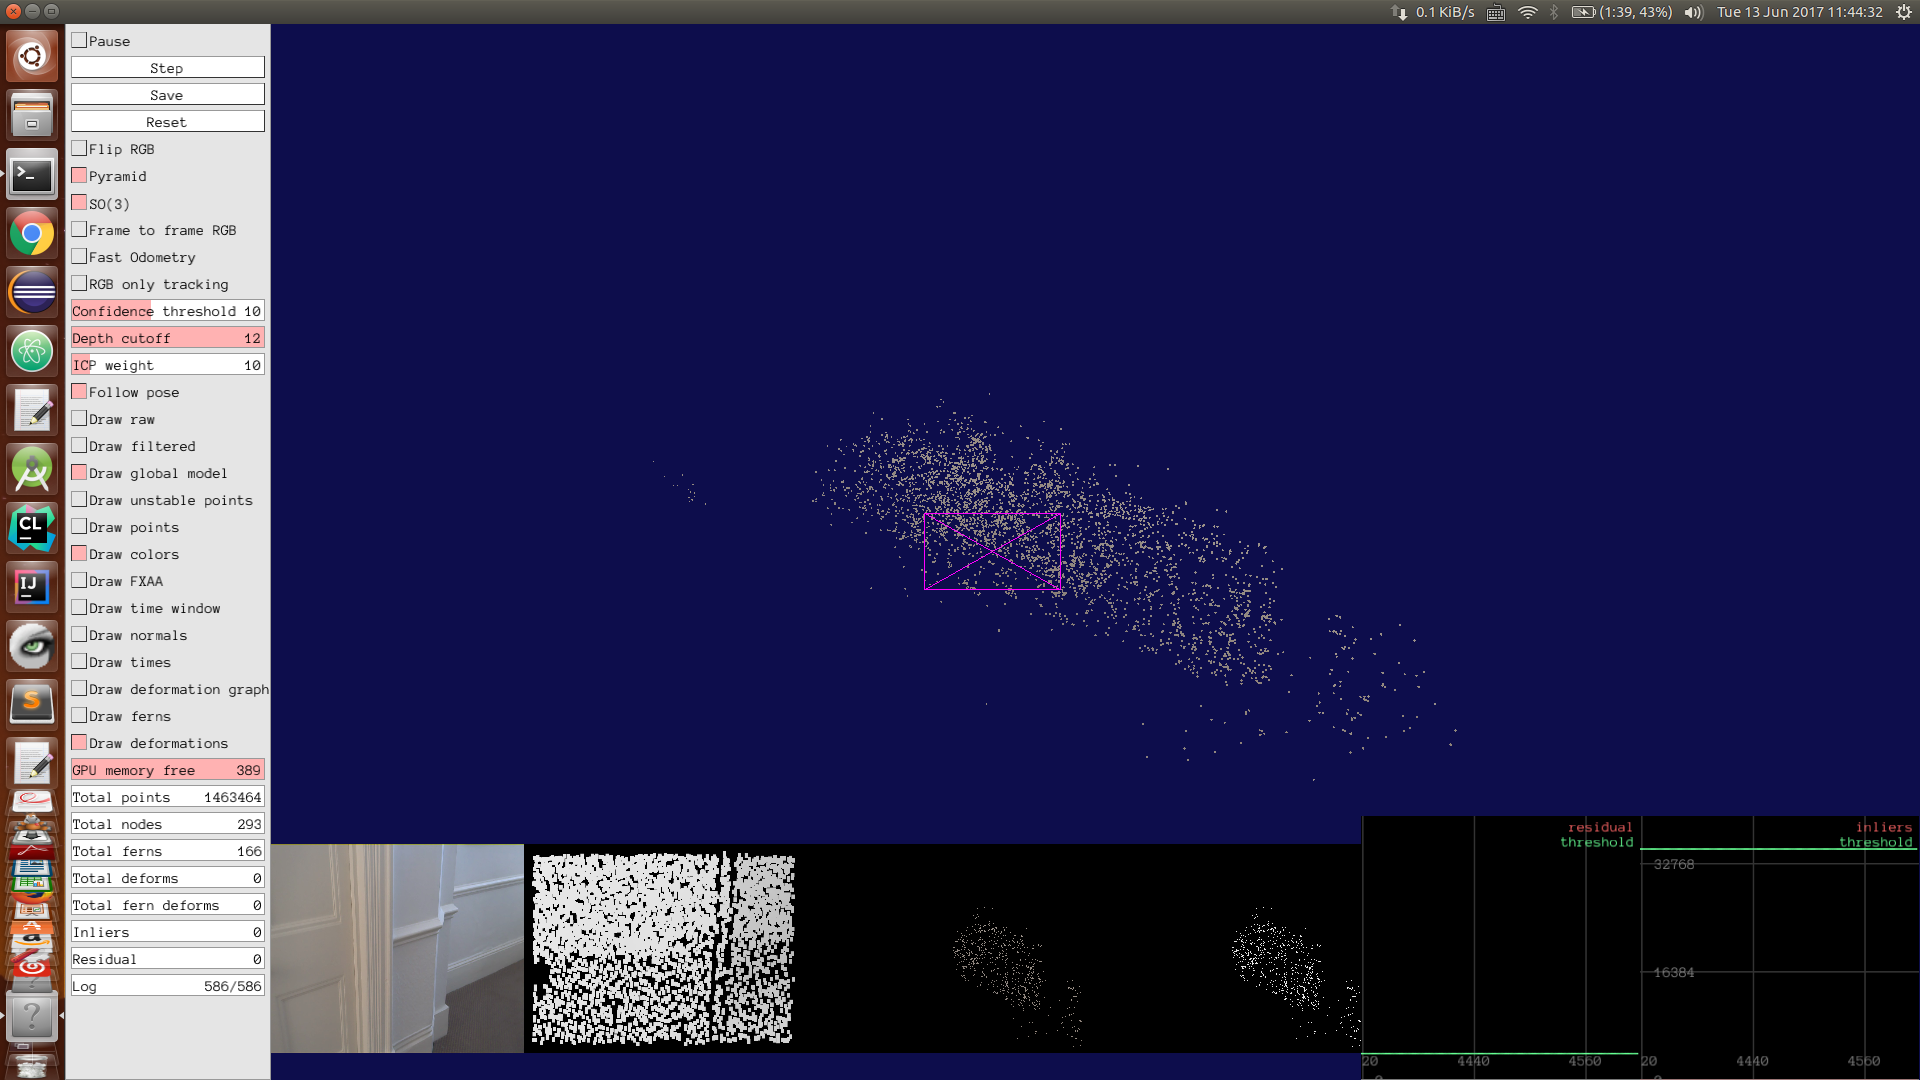
\includegraphics[width=0.7\textwidth]{figures/Screenshot10}
    \caption{Screenshot10}
    \label{fig:Screenshot10}
\end{figure}

\begin{figure}[h]
    \centering
    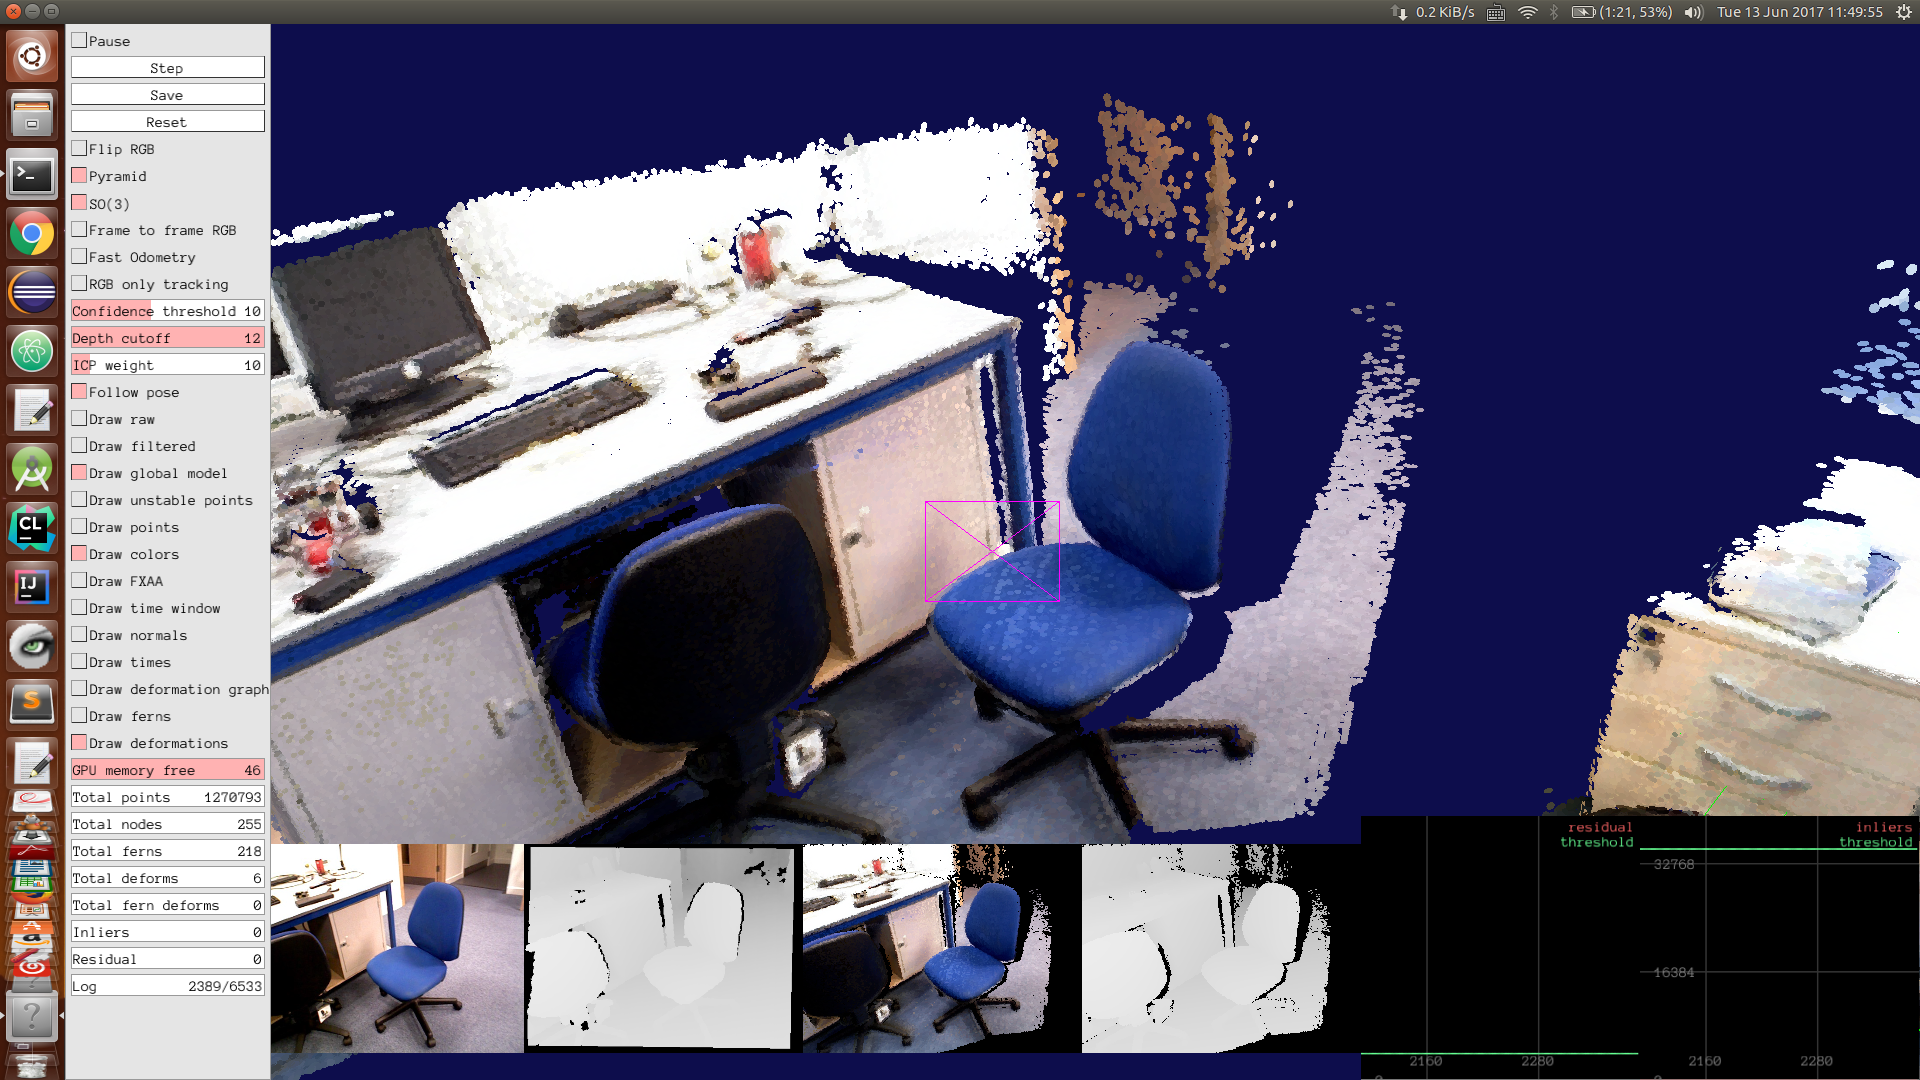
\includegraphics[width=0.7\textwidth]{figures/Screenshot11}
    \caption{Screenshot11}
    \label{fig:Screenshot11}
\end{figure}


\begin{figure}[h]
    \centering
    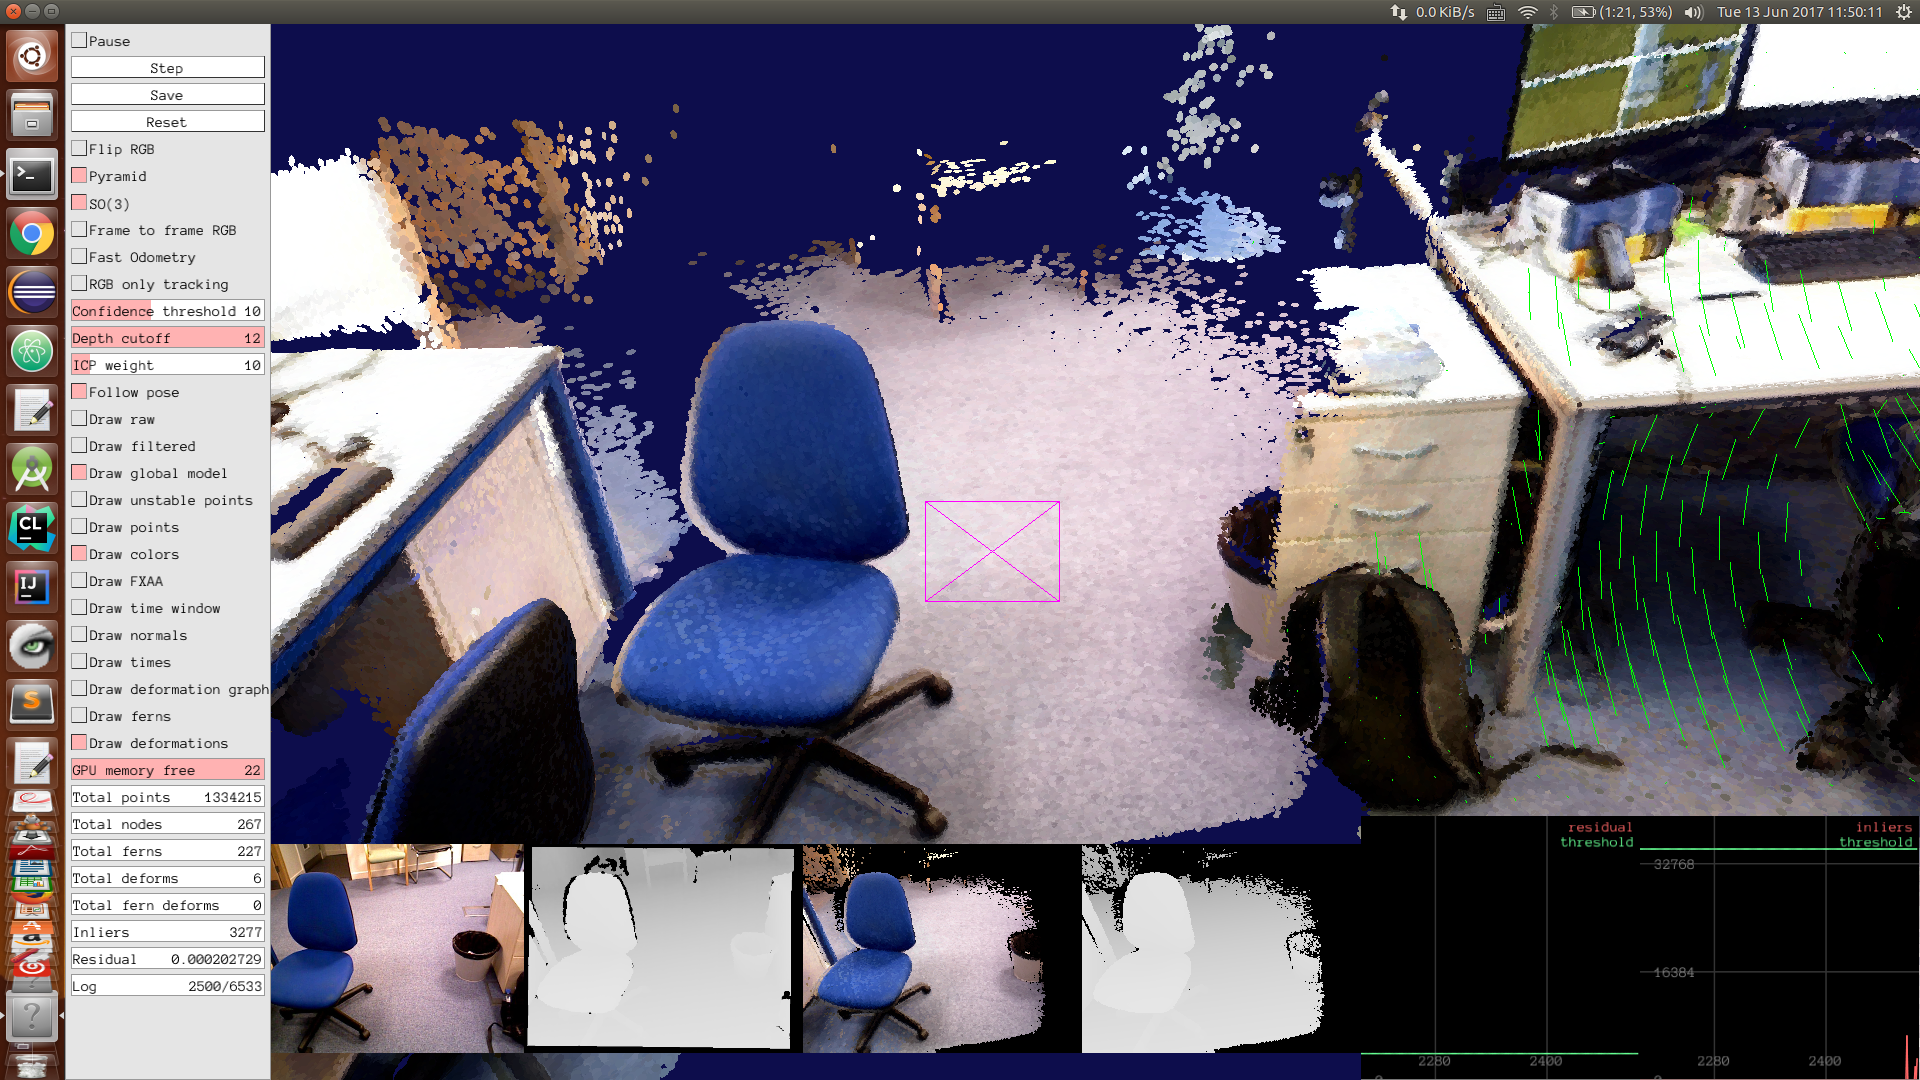
\includegraphics[width=0.7\textwidth]{figures/Screenshot14}
    \caption{Screenshot14}
    \label{fig:Screenshot14}
\end{figure}



\begin{figure}[h]
    \centering
    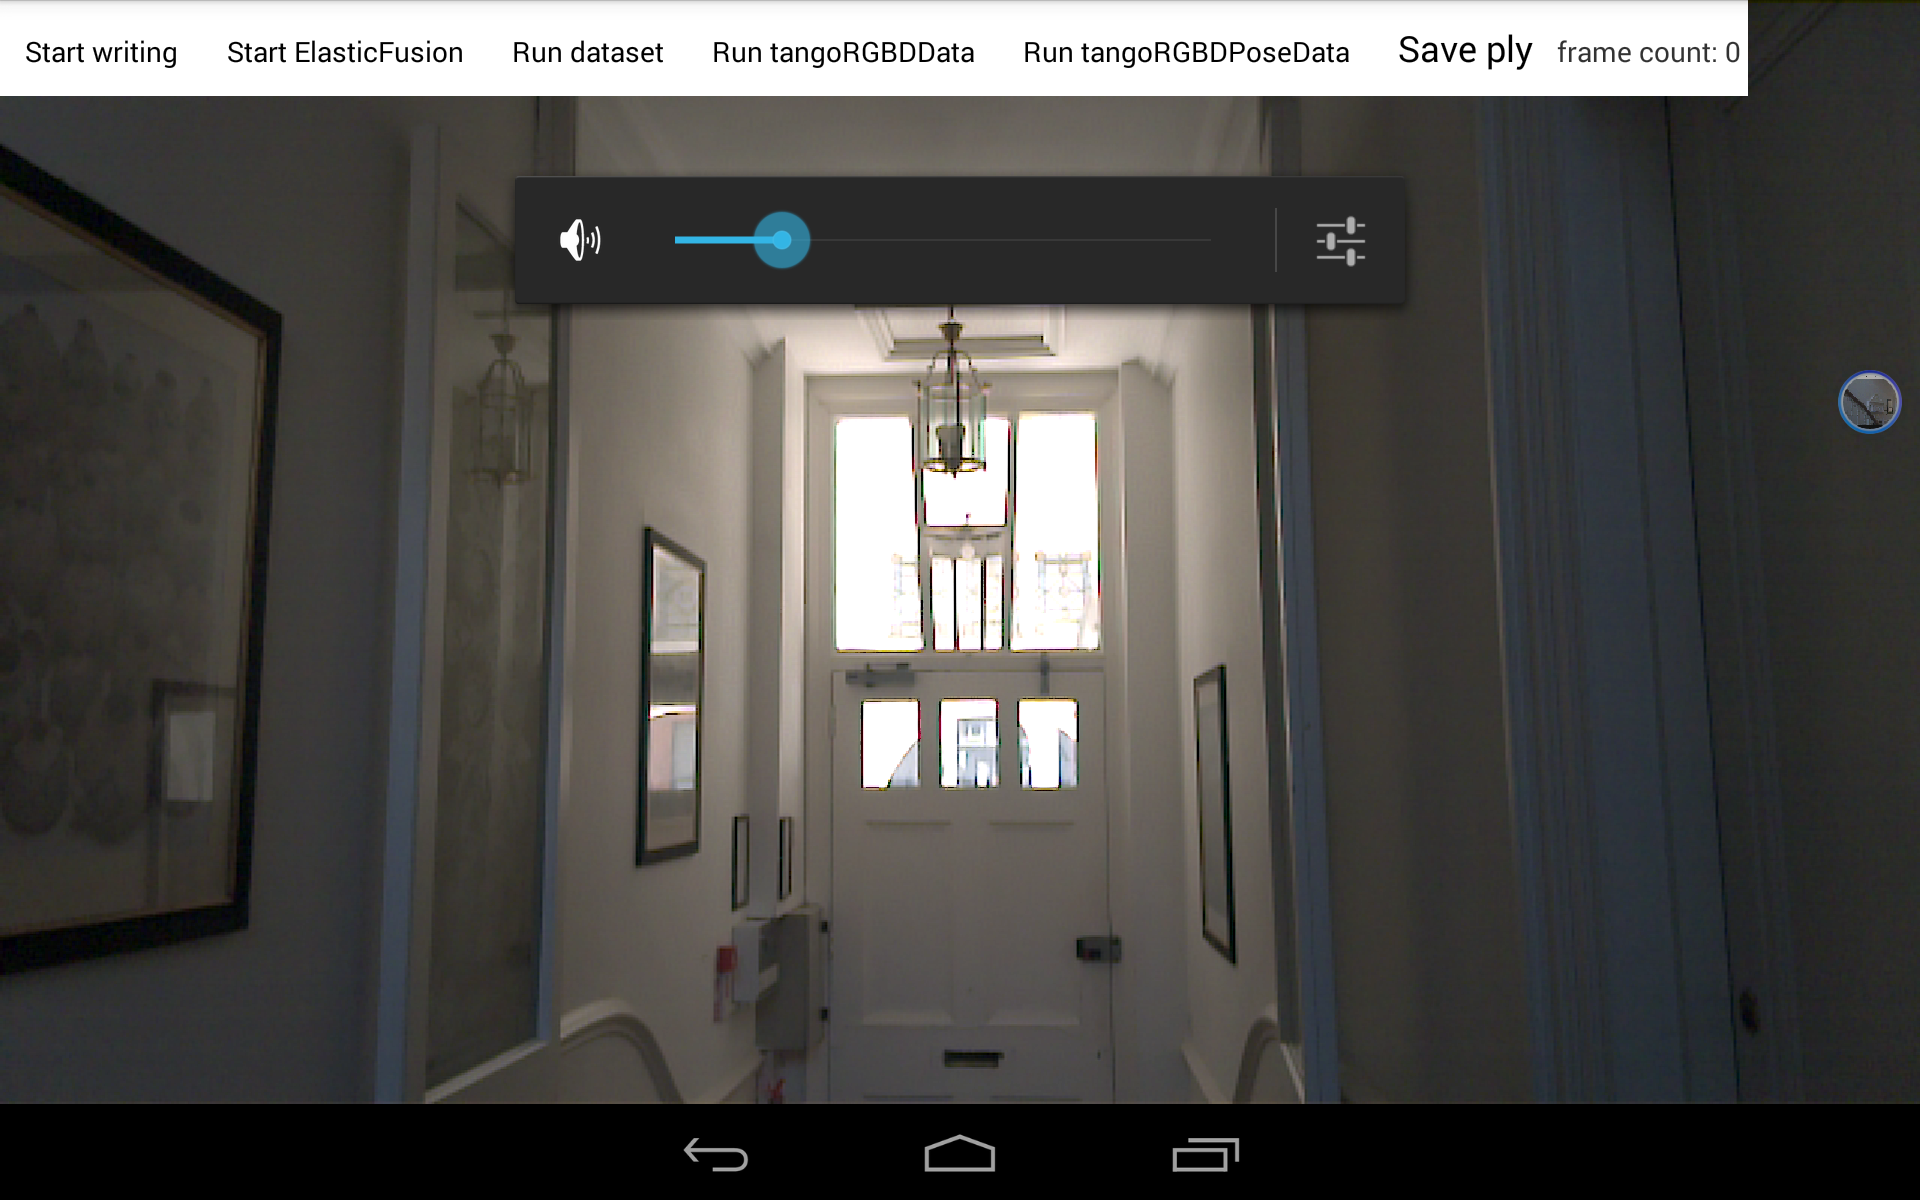
\includegraphics[width=0.7\textwidth]{figures/ScreenshotTango1}
    \caption{ScreenshotTango1}
    \label{fig:ScreenshotTango1}
\end{figure}




\newpage


The project timeline is shown in Fig \ref{fig:tiemline2} with each task corresponding to a stage above.

\begin{figure}
\centering
    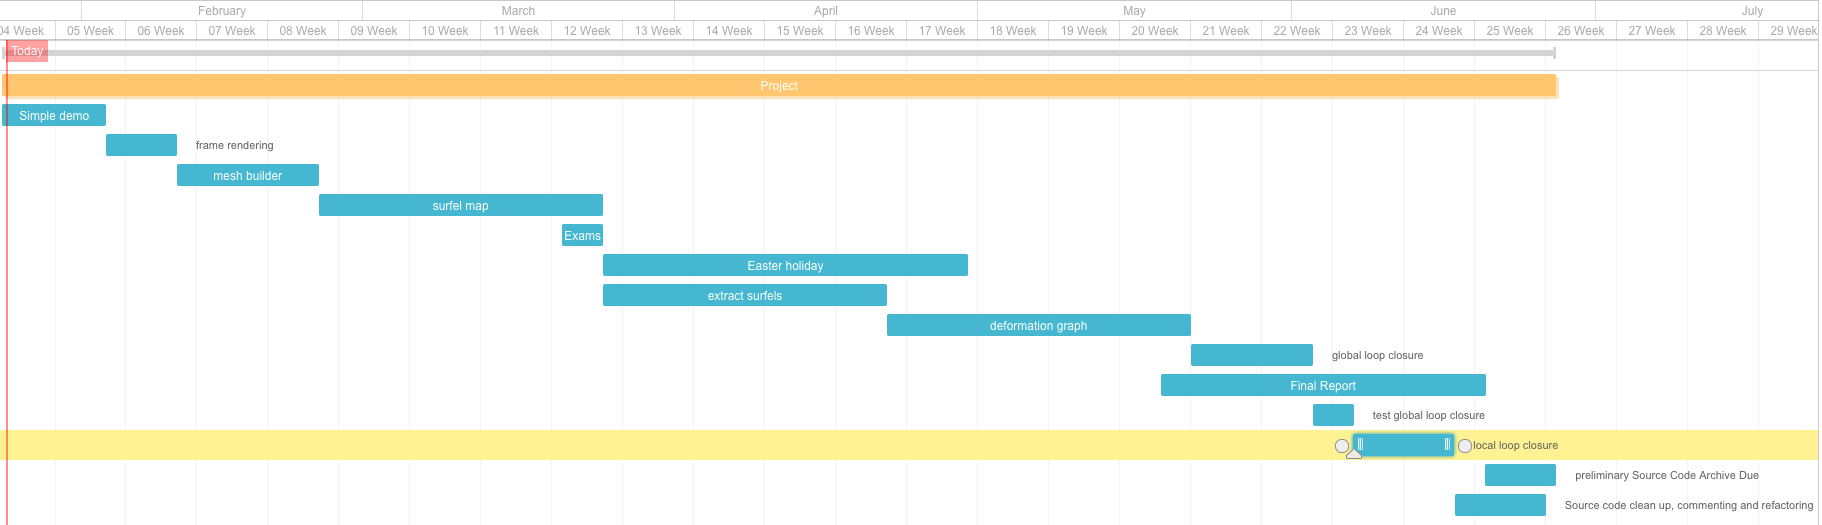
\includegraphics[angle=90,width=\textwidth,height=\textheight,keepaspectratio]{figures/timeline2}
   \caption{Graph for project timeline}
    \label{fig:tiemline2}
\end{figure}

\newpage


\section{Evaluation}


\subsection{Reconstruction Accuracy}



Nvidia Tegra K1  approx = GT620-GT540\\
\\
make it faster: Kintinuous will run at 30Hz on a modern laptop on battery power these days). You can try disabling SO(3) pre-alignment, enabling fast odometry, only using either ICP or RGB tracking and not both, running in open loop mode or disabling the tracking pyramid. All of these will cost you accuracy.\\
\\
Nvidia Tegra K1  192  GPU core, Direct3D 12, OpenGL ES 3.1, CUDA 6.5, OpenGL 4.4/OpenGL 4.5, and Vulkan, 365 G FLOPS, 192 CUDA cores * 2 FLOPS per core * 950MHz, sm30, floating point operations per second (FLOPS)\\
laptop: GTX765M PICe SSE2 , 1224 GFLOPS\\
In this project, only the core part of ElasticFusion is used, the original dependency of Pangolin is removed and replaced with plain OpenGL ES code that full fills the same function, other necessary change is made to enable the ElasticFusion program be run on Android platform. When the user starts ElasticFusion on the Tango tablet, a new ElasticFusion thread is started and it takes RGBD and pose data from the circular buffer previously mentioned, and use these frame data as the input to the program.\\






\subsection{depth sensor noise}

,depth点非常sparse。








\subsection{Computation power problem}











\subsection{Optimization problem}

Be warned that many projects fall down through poor evaluation. Simply building a system and documenting its design and functionality is not enough to gain top marks. It is extremely important that you evaluate what you have done both in absolute terms and in comparison with existing techniques, software, hardware etc. This might involve quantitative evaluation, for example based on numerical results, performance etc. or something more qualitative such as expressibility, functionality, ease-of-use etc. At some point you should also evaluate the strengths and weaknesses of what you have done. Avoid statements like "The project has been a complete success and we have solved all the problems asssociated with blah...; - you will be shot down immediately! It is important to understand that there is no such thing as a perfect project. Even the very best pieces of work have their limitations and you are expected to provide a proper critical appraisal of what you have done.\\

=============\\




The evaluation of this project is intended to use the same mechanism as in original ElasticFusion\citep{whelan2016elasticfusion} paper, as the goal of this project is to deploying this algorithm on Google Tango tablet.\\
In order to measure the performance of this solution by quantity and quality. Both algorithm and computational performance need to be benchmarked.\\
Both
A. Trajectory Estimation
To evaluate the trajectory estimation performance of our approach
we test our system on the RGB-D benchmark of Sturm
et al. [22]. This benchmark provides synchronised ground truth
poses for an RGB-D sensor moved through a scene, captured
with a highly precise motion capture system.  We use the absolute
trajectory (ATE) root-mean-square error metric (RMSE) in
our comparison, which measures the root-mean-square of the
Euclidean distances between all estimated camera poses and
the ground truth poses associated by timestamp [22].


B. Surface Estimation
We evaluate the surface reconstruction results of our approach
on the
 This
benchmark provides ground truth poses for a camera moved
through a synthetic environment as well as a ground truth 3D
model which can be used to evaluate surface reconstruction
accuracy.

Computational Performance


​The evaluation of this project is intended to use the same mechanism as in original ElasticFusion\citep{whelan2016elasticfusion} paper, as the goal of this project is to deploying this algorithm on Google Tango tablet.\\
In order to measure the performance of this solution by quantity and quality. Both algorithm and computational performance need to be benchmarked.\\
For the algorithm, trajectory accuracy can be tested using sample data sets to provide RGB-D input, then the trajectory output can be compared with the ground truth data that is obtained by using industrial standard system. The root mean square distance between every estimated pose and ground truth pose can be calculated to provide error at each timepoint. In the 3D reconstruction part, similar method can be used to compare the reconstructed surface to benchmark data for accuracy estimation. However, since the post data and image input are provided by Tango platform, a way is needed to fed the benchmark data into Tango.\\
For computational Performance, we can simply plot the frame rate during the process of 3D scanning to check if it is within the acceptable range for real time SLAM algorithm.\\
​The evaluation of this project is intended to use the same mechanism as in original ElasticFusion\citep{whelan2016elasticfusion} paper, as the goal of this project is to deploying this algorithm on Google Tango tablet.\\
In order to measure the performance of this solution by quantity and quality. Both algorithm and computational performance need to be benchmarked.\\
For the algorithm, trajectory accuracy can be tested using sample data sets to provide RGB-D input, then the trajectory output can be compared with the ground truth data that is obtained by using industrial standard system. The root mean square distance between every estimated pose and ground truth pose can be calculated to provide error at each timepoint. In the 3D reconstruction part, similar method can be used to compare the reconstructed surface to benchmark data for accuracy estimation. However, since the post data and image input are provided by Tango platform, a way is needed to fed the benchmark data into Tango.\\
For computational Performance, we can simply plot the frame rate during the process of 3D scanning to check if it is within the acceptable range for real time SLAM algorithm.



\subsubsection{Software limitation}






\newpage







\section{Conclusions and Future Work}

The project's conclusions should list the things which have been learnt as a result of the work you have done. For example, "The use of overloading in C++ provides a very elegant mechanism for transparent parallelisation of sequential programs", or "The overheads of linear-time n-body algorithms makes them computationally less efficient than O(n log n) algorithms for systems with less than 100000 particles". Avoid tedious personal reflections like "I learned a lot about C++ programming...", or "Simulating colliding galaxies can be real fun...". It is common to finish the report by listing ways in which the project can be taken further. This might, for example, be a plan for doing the project better if you had a chance to do it again, turning the project deliverables into a more polished end product, or extending the project into a programme for an MPhil or PhD.\\

ASUS ZenFone AR\\

optimization \\
slow, GPU, memmory\\
resolution, \\
\\
However, extension and optimization could be done if more time is given and basic solution is completed. Until here the 3D reconstruction process will be running on Tango tablet's NVIDIA Tegra K1 processor without utilizing the CUDA feature on it to improve performance by parallel processing. A optimization could be to use CUDA in the camera tracking process. Also on the application side, extra features can be added such as saving the reconstructed surfel map on the Tango tablet, add an interactive view of reconstructed 3D surface map on the screen to allow for drag and zoom operation, showing the camera's current pose on the map. Further more, demo application and be built to utilising the augmented reality ability on Tango platform, such as placing a virtual static object on the 3D reconstructing surface.\\



\newpage




\section{Bibliography}



This consists of a list of all the books, articles, manuals etc. used in the project and referred to in the report. You should provide enough information to allow the reader to find the source. In particular references must contain all the information regarding the publication of the paper and must be consistently formatted. Usually this means:\\
* For journals: Authors, Title, Journal, volume number, issue number, page number, publisher, month, year.
* For conferences: Authors, Title, Conference name, Place where held, publisher, page number, month, year.
* For technical reports: Authors, Title, institution, Technical report number, month, year.
* For web references: Authors, Title, Web-reference, date accessed.
* URLs are optional for published work but preferred.\\
A weakness of many reports is inadequate citation of a source of information. It's easy to get this right so there are no excuses. Each entry in the bibliography should list the author(s) and title of the piece of work and should give full details of where it can be found. For example:\\
1 Bennett, A.J., Field, A.J. and Harrison, P.G., "Modelling and Validation of Shared Memory Coherency Protocols", Performance Evaluation, 1996, Vol. 27  28, 1996, pp. 541-562. rather than just listing the source as "Performance Evaluation 1996".
Using a reference management programme can make your life simpler.See for example Bibdesk,JabRef,RefWorks, etc.\\


\newpage





\section{Appendix}


The appendices contain information which is peripheral to the main body of the report. Information typically included are things like parts of the code, tables, proofs, test cases or any other material which would break up the theme of the text if it appeared in situ. You should try to bind all your material in a single volume if possible.\\

\newpage





\section{User Guide}



For projects which result in a new piece of software you should provide a proper user guide providing easily understood instructions on how to use it. A particularly useful approach is to treat the user guide as a walk-through of a typical session, or set of sessions, which collectively display all the features of your system. Technical details of how the package works should be in the body of the report. Keep it concise and simple. The extensive use of diagrams illustrating the package in action prove particularly helpful. The user guide is sometimes included as a chapter in the main body of the report, but is often better in an appendix.\\


\newpage





\section{Program Listings}


Complete program listings should NOT be part of the report except in specific cases at the request of your supervisor. The project report(s) must be bound in a departmental folder and must include a standard title page produced by the project co-ordinator. More of this nearer the date.\\
You are strongly advised to spend some time looking at the reports of previous project students to get a feel for what's good and bad. In June 1999 we introduced a "Distinguished Project" classification, which is a formal recognition of outstanding projects for which no official prize was awarded. The complete list of prize winners and the other distinguished projects, along with links to the final reports, can be found here.\\

\newpage

\section{Word Count}



There is no word count for the report as such, but ideally you should not exceed the limit of 40,000 words. Generally, our best projects tend to have the word count in the range of 20,000 - 35,000 words with a few going beyond that. This does not include the Appendices.\\



\bibliographystyle{unsrt}
\bibliography{mybi}

\end{document}
%%% Local Variables:
%%% mode: latex
%%% TeX-master: t
%%% End:
